% =========================================================
% Breadcrumb
% =========================================================
\begin{tcolorbox}[
  colback=gray!6,
  colframe=gray!40,
  arc=2pt,
  left=8pt, right=8pt, top=6pt, bottom=6pt,
  title={\small\textbf{Where You Are in the Journey}},
  fonttitle=\small\bfseries
]
\begin{center}
\small
Propositional Logic
$\;\to\;$ Predicate Calculus
$\;\to\;$ Sets \& Functions
$\;\to\;$ Proof Techniques
$\;\to\;$ Axiom Systems
$\;\to\;$ $\mathbb{N}$, $\mathbb{Z}$, $\mathbb{Q}$
$\;\to\;$ \textbf{Real Numbers ($\mathbb{R}$)}
$\;\to\;$ Real Analysis
$\;\to\;$ $\cdots$
\end{center}

\medskip
\noindent\textbf{How we got here.}
The rational numbers gave us a dense ordered field, but they contain gaps:
there is no $q \in \mathbb{Q}$ with $q^2 = 2$.
The real number system fills these gaps. Two rigorous constructions achieve
this --- Dedekind cuts and Cauchy sequences --- and both yield the same
unique complete ordered field.

\medskip
\noindent\textbf{What this chapter builds.}
The axiomatic structure of $\mathbb{R}$: field axioms, order axioms,
the completeness axiom, and their immediate consequences ---
the Archimedean property, density of $\mathbb{Q}$, and the
interval and bound theory that underpins all of analysis.
We also study how $\mathbb{R}$ is \emph{constructed} from $\mathbb{Q}$
via Dedekind cuts and Cauchy sequences.

\medskip
\noindent\textbf{Where this leads.}
Real analysis in Volume~III takes $\mathbb{R}$ as given and develops
sequences, series, convergence, and their limiting behaviour.
The field and order axioms established here propagate unchanged
into metric spaces, normed spaces, and abstract algebra.
\end{tcolorbox}
\vspace{1em}

% =========================================================
% Structural Roadmap
% =========================================================
\subsection*{Structural Roadmap}

This chapter covers the \emph{algebraic and analytic axioms} of
$\mathbb{R}$ and the \emph{constructions} that justify its existence.
Sequence and series theory is developed in
\textbf{Volume~III, Real Analysis}.

\begin{center}
\textbf{Axioms $\longrightarrow$ Order \& Bounds
$\longrightarrow$ Completeness $\longrightarrow$ Constructions}
\end{center}

The global progression is:
\begin{enumerate}
  \item Field and order axioms
  \item Intervals and convexity
  \item Bounds: upper/lower bounds, maximum, minimum
  \item Extremal values: supremum and infimum
  \item Completeness: the least upper bound property and its consequences
  \item Constructions of $\mathbb{R}$: Dedekind cuts
  \item Constructions of $\mathbb{R}$: Cauchy sequences
  \item Interval arithmetic
\end{enumerate}

\vspace{1em}

\begin{remark}[Primary sources]
Axiomatic development follows Abbott, \textit{Understanding Analysis}
and Ross, \textit{Elementary Analysis}.
The Cauchy sequence construction follows Tao, \textit{Analysis~I},
Chapters~5--6.
The Dedekind cut construction follows Rudin,
\textit{Principles of Mathematical Analysis}, Appendix to Chapter~1.
\end{remark}

% =========================================================
% Content
% =========================================================
% =========================================================
% Real Numbers (ℝ) — Notes Master Index
% =========================================================
% =========================================================
% Real Numbers — Foundations
% Axioms, intervals, bounds, completeness
% =========================================================
% =========================================================
% Axioms of the Real Numbers
% File: notes-axioms-of-the-reals.tex
% =========================================================

\subsection{Axioms of the Real Numbers}

% ---------------------------------------------------------
% Toolkit
% ---------------------------------------------------------
\begin{tcolorbox}[colback=gray!6, colframe=gray!40, arc=2pt,
  left=6pt, right=6pt, top=4pt, bottom=4pt,
  title={\small\textbf{Axioms Of The Reals — Quick Reference}},
  fonttitle=\small\bfseries]
\begin{tabular}{@{}p{0.28\textwidth}p{0.68\textwidth}@{}}
\textbf{Core items} & Key definitions/results introduced in this file.\\
\textbf{How to use} & Read the boxed items first; proofs and consequences follow.\\
\textbf{Dependencies} & Refer back to earlier sections as needed.\\
\end{tabular}
\end{tcolorbox}


The real numbers $\mathbb{R}$ form a \emph{totally ordered field}.
This structure consists of:

\begin{itemize}
\item Field axioms (algebraic structure),
\item Order axioms (order structure),
\item Completeness axiom (analytic structure).
\end{itemize}

% ---------------------------------------------------------
\subsubsection{Basic Definitions}

\begin{remark}
A \emph{field} is a set equipped with two binary operations,
addition $(+)$ and multiplication $(\cdot)$,
satisfying closure, associativity, commutativity,
identity, inverse, and distributive laws.

An \emph{ordered field} is a field equipped with a total order
compatible with the algebraic operations.
\end{remark}

% ---------------------------------------------------------
\subsubsection{Main Theorems (Axioms)}

% =========================================================
% Field Axioms
% =========================================================

\paragraph{Additive Axioms}

\begin{description}

\item[\textbf{Axiom A1 (Additive Closure).}]
\[
\forall x \forall y \, (x,y \in \mathbb{R} \rightarrow x+y \in \mathbb{R})
\]

\item[\textbf{Axiom A2 (Additive Commutativity).}]
\[
\forall x \forall y \, (x+y = y+x)
\]

\item[\textbf{Axiom A3 (Additive Associativity).}]
\[
\forall x \forall y \forall z \, ((x+y)+z = x+(y+z))
\]

\item[\textbf{Axiom A4 (Additive Identity).}]
\[
\exists 0 \, \forall x \, (x+0 = x)
\]

\item[\textbf{Axiom A5 (Additive Inverse).}]
\[
\forall x \, \exists y \, (x+y = 0)
\]

\end{description}

\paragraph{Multiplicative Axioms}

\begin{description}

\item[\textbf{Axiom M1 (Multiplicative Closure).}]
\[
\forall x \forall y \, (x,y \in \mathbb{R} \rightarrow x\cdot y \in \mathbb{R})
\]

\item[\textbf{Axiom M2 (Multiplicative Commutativity).}]
\[
\forall x \forall y \, (x\cdot y = y\cdot x)
\]

\item[\textbf{Axiom M3 (Multiplicative Associativity).}]
\[
\forall x \forall y \forall z \, ((x\cdot y)\cdot z = x\cdot (y\cdot z))
\]

\item[\textbf{Axiom M4 (Multiplicative Identity).}]
\[
\exists 1 \, (1 \neq 0 \wedge \forall x \, (x\cdot 1 = x))
\]

\item[\textbf{Axiom M5 (Multiplicative Inverse).}]
\[
\forall x \, (x \neq 0 \rightarrow \exists y \, (x\cdot y = 1))
\]

\end{description}

\paragraph{Distributive Axiom}

\begin{description}

\item[\textbf{Axiom D (Distributivity).}]
\[
\forall x \forall y \forall z \, (x\cdot (y+z) = x\cdot y + x\cdot z)
\]

\end{description}

% =========================================================
% Order Axioms
% =========================================================

\paragraph{Linear Order Axioms}

\begin{description}

\item[\textbf{O1 (Reflexivity).}]
\[
\forall x\in\mathbb{R},\quad x \le x
\]

\item[\textbf{O2 (Antisymmetry).}]
\[
\forall x,y\in\mathbb{R},\quad
(x \le y \wedge y \le x) \rightarrow x = y
\]

\item[\textbf{O3 (Transitivity).}]
\[
\forall x,y,z\in\mathbb{R},\quad
(x \le y \wedge y \le z) \rightarrow x \le z
\]

\item[\textbf{O4 (Totality / Comparability).}]
\[
\forall x,y\in\mathbb{R},\quad
x \le y \ \vee\ y \le x
\]

\end{description}

The strict order is defined by:
\[
x < y
\quad\text{iff}\quad
x \le y \text{ and } x \neq y.
\]

\paragraph{Compatibility with Field Operations}

\begin{description}

\item[\textbf{O5 (Additive Monotonicity).}]
\[
\forall x,y,z\in\mathbb{R},\quad
x \le y \rightarrow x+z \le y+z
\]

\item[\textbf{O6 (Multiplicative Monotonicity for Nonnegative Factors).}]
\[
\forall x,y,z\in\mathbb{R},\quad
(x \le y \wedge 0 \le z) \rightarrow xz \le yz
\]

\item[\textbf{O7 (Positivity of the Unit).}]
\[
0 < 1
\]

\end{description}

\begin{remark}
Axiom O6 implies that multiplication by a negative number reverses
inequalities; this will later be proved as a theorem.
\end{remark}

% ---------------------------------------------------------
\subsubsection{Consequences}

The logical implication of this entire section is:

\[
\text{Field Axioms}
\Rightarrow
\text{Algebraic Structure}
\]

\[
\text{Field + Order Axioms}
\Rightarrow
\text{Ordered Field}
\]

To uniquely characterize $\mathbb{R}$ among ordered fields,
one must additionally assume:

\[
\textbf{Completeness}.
\]

\begin{remark}[Logical Structure]
\[
\text{Field}
\Rightarrow
\text{Ordered Field}
\Rightarrow
\text{Complete Ordered Field}.
\]

The real numbers $\mathbb{R}$ are the unique (up to isomorphism)
complete ordered field.
\end{remark}

% =========================================================
% Intervals
% =========================================================

\subsection{Intervals in the Real Numbers}

% ---------------------------------------------------------
% Toolkit
% ---------------------------------------------------------
\begin{tcolorbox}[colback=gray!6, colframe=gray!40, arc=2pt,
  left=6pt, right=6pt, top=4pt, bottom=4pt,
  title={\small\textbf{Intervals — Quick Reference}},
  fonttitle=\small\bfseries]
\begin{tabular}{@{}p{0.28\textwidth}p{0.68\textwidth}@{}}
\textbf{Core items} & Key definitions/results introduced in this file.\\
\textbf{How to use} & Read the boxed items first; proofs and consequences follow.\\
\textbf{Dependencies} & Refer back to earlier sections as needed.\\
\end{tabular}
\end{tcolorbox}


Intervals are fundamental subsets of the real line defined using the order
relation on $\mathbb{R}$. Let $a,b \in \mathbb{R}$ with $a < b$.

% ---------------------------------------------------------
\subsubsection{Basic Definitions}
% ---------------------------------------------------------

\subsubsection*{Bounded Intervals}

\begin{tcolorbox}[colback=propbox, colframe=propborder, arc=2pt,
  left=6pt, right=6pt, top=4pt, bottom=4pt,
  title={\small\textbf{Definition (Open Interval)}},
  fonttitle=\small\bfseries]
The \emph{open interval} from $a$ to $b$ is the set
\[
(a,b) := \{ x \in \mathbb{R} : a < x < b \}.
\]
\[
\forall x \, (x \in (a,b) \leftrightarrow a < x \wedge x < b)
\]
\end{tcolorbox}

\begin{tcolorbox}[colback=propbox, colframe=propborder, arc=2pt,
  left=6pt, right=6pt, top=4pt, bottom=4pt,
  title={\small\textbf{Definition (Closed Interval)}},
  fonttitle=\small\bfseries]
The \emph{closed interval} from $a$ to $b$ is the set
\[
[a,b] := \{ x \in \mathbb{R} : a \le x \le b \}.
\]
\[
\forall x \, (x \in [a,b] \leftrightarrow a \le x \wedge x \le b)
\]
\end{tcolorbox}

\begin{tcolorbox}[colback=propbox, colframe=propborder, arc=2pt,
  left=6pt, right=6pt, top=4pt, bottom=4pt,
  title={\small\textbf{Definition (Half-Open Intervals)}},
  fonttitle=\small\bfseries]
The \emph{left-closed, right-open interval} is
\[
[a,b) := \{ x \in \mathbb{R} : a \le x < b \}.
\]
The \emph{left-open, right-closed interval} is
\[
(a,b] := \{ x \in \mathbb{R} : a < x \le b \}.
\]
\end{tcolorbox}

\subsubsection*{Unbounded Intervals}

\begin{tcolorbox}[colback=propbox, colframe=propborder, arc=2pt,
  left=6pt, right=6pt, top=4pt, bottom=4pt,
  title={\small\textbf{Definition (Open Rays)}},
  fonttitle=\small\bfseries]
The \emph{open rays} determined by $a \in \mathbb{R}$ are
\[
(a,\infty) := \{ x \in \mathbb{R} : x > a \},
\qquad
(-\infty,a) := \{ x \in \mathbb{R} : x < a \}.
\]
\end{tcolorbox}

\begin{tcolorbox}[colback=propbox, colframe=propborder, arc=2pt,
  left=6pt, right=6pt, top=4pt, bottom=4pt,
  title={\small\textbf{Definition (Closed Rays)}},
  fonttitle=\small\bfseries]
The \emph{closed rays} determined by $a \in \mathbb{R}$ are
\[
[a,\infty) := \{ x \in \mathbb{R} : x \ge a \},
\qquad
(-\infty,a] := \{ x \in \mathbb{R} : x \le a \}.
\]
\end{tcolorbox}

\subsubsection*{Degenerate and Trivial Intervals}

\begin{tcolorbox}[colback=propbox, colframe=propborder, arc=2pt,
  left=6pt, right=6pt, top=4pt, bottom=4pt,
  title={\small\textbf{Definition (Degenerate Interval)}},
  fonttitle=\small\bfseries]
If $a=b$, the closed interval
\[
[a,a] = \{a\}
\]
is called a \emph{degenerate interval}.
\end{tcolorbox}

\begin{tcolorbox}[colback=propbox, colframe=propborder, arc=2pt,
  left=6pt, right=6pt, top=4pt, bottom=4pt,
  title={\small\textbf{Definition (Empty Interval)}},
  fonttitle=\small\bfseries]
If $a>b$, the set
\[
(a,b) = \varnothing
\]
is called an \emph{empty interval}.
\end{tcolorbox}

% ---------------------------------------------------------
\subsubsection{Main Theorems}
% ---------------------------------------------------------

\begin{theorem}[Characterization of Intervals]
A subset $I \subseteq \mathbb{R}$ is an interval if and only if
whenever $x,z \in I$ and $x < y < z$, then $y \in I$.
Equivalently,
\[
\forall x,z \in I,\; x<z \Rightarrow
\bigl(
\forall y \in \mathbb{R},\;
(x<y<z \Rightarrow y \in I)
\bigr).
\]
\end{theorem}

\begin{proof}
($\Rightarrow$) Each of the standard interval forms defined above
contains every real number between any two of its elements by definition.

($\Leftarrow$) Suppose $I$ satisfies the stated property.
Let $a = \inf I$ and $b = \sup I$ in the extended real line.
Using the order axioms and the interval property, one verifies that
$I$ must be one of the standard forms:
\[
(a,b),\ [a,b],\ (a,b],\ [a,b),
\]
or one of the unbounded variants.
\qed
\end{proof}

\begin{remark}
Intervals are precisely the subsets of $\mathbb{R}$ with the property that if
$x<y<z$ and $x,z$ belong to the set, then $y$ also belongs to the set.
\end{remark}

% ---------------------------------------------------------
\subsubsection{Consequences}
% ---------------------------------------------------------

The logical implication of this section is:

\[
\text{Order Structure of }\mathbb{R}
\Rightarrow
\text{Intervals}
\Rightarrow
\text{Convex subsets of }\mathbb{R}.
\]

Intervals encode the idea of “no gaps” between points of a set.
They are the basic building blocks for:

\begin{itemize}
\item neighborhoods,
\item open sets,
\item topology of $\mathbb{R}$,
\item and completeness arguments (e.g. nested intervals).
\end{itemize}

\begin{remark}[Logical Structure]
The major structural flow is:

\[
\text{Field Axioms}
\Rightarrow
\text{Order Axioms}
\Rightarrow
\text{Definition of Intervals}
\Rightarrow
\text{Convexity Property}
\Rightarrow
\text{Topological Structure of }\mathbb{R}.
\]
\end{remark}

% =========================================================
% Bounds and Extremal Values (Set-Theoretic)
% =========================================================

\subsection{Bounds and Extremal Values}

% ---------------------------------------------------------
% Toolkit
% ---------------------------------------------------------
\begin{tcolorbox}[colback=gray!6, colframe=gray!40, arc=2pt,
  left=6pt, right=6pt, top=4pt, bottom=4pt,
  title={\small\textbf{Bounds — Quick Reference}},
  fonttitle=\small\bfseries]
\begin{tabular}{@{}p{0.28\textwidth}p{0.68\textwidth}@{}}
\textbf{Core items} & Key definitions/results introduced in this file.\\
\textbf{How to use} & Read the boxed items first; proofs and consequences follow.\\
\textbf{Dependencies} & Refer back to earlier sections as needed.\\
\end{tabular}
\end{tcolorbox}

\label{sec:bounds}

% ---------------------------------------------------------
\subsubsection{Basic Definitions}

\begin{tcolorbox}[colback=propbox, colframe=propborder, arc=2pt,
  left=6pt, right=6pt, top=4pt, bottom=4pt,
  title={\small\textbf{Definition (Upper Bound)}},
  fonttitle=\small\bfseries]
Let $A \subseteq \mathbb{R}$.
A number $u \in \mathbb{R}$ is an \emph{upper bound} for $A$ if
\[
\forall a \in A,\quad a \le u.
\]
\end{tcolorbox}

\begin{tcolorbox}[colback=propbox, colframe=propborder, arc=2pt,
  left=6pt, right=6pt, top=4pt, bottom=4pt,
  title={\small\textbf{Definition (Lower Bound)}},
  fonttitle=\small\bfseries]
Let $A \subseteq \mathbb{R}$.
A number $\ell \in \mathbb{R}$ is a \emph{lower bound} for $A$ if
\[
\forall a \in A,\quad \ell \le a.
\]
\end{tcolorbox}

\begin{tcolorbox}[colback=propbox, colframe=propborder, arc=2pt,
  left=6pt, right=6pt, top=4pt, bottom=4pt,
  title={\small\textbf{Definition (Bounded Above / Below)}},
  fonttitle=\small\bfseries]
A set $A \subseteq \mathbb{R}$ is said to be:
\begin{itemize}
  \item \emph{bounded above} if it has at least one upper bound;
  \item \emph{bounded below} if it has at least one lower bound;
  \item \emph{bounded} if it is both bounded above and bounded below.
\end{itemize}
\end{tcolorbox}

\begin{tcolorbox}[colback=propbox, colframe=propborder, arc=2pt,
  left=6pt, right=6pt, top=4pt, bottom=4pt,
  title={\small\textbf{Definition (Maximum)}},
  fonttitle=\small\bfseries]
Let $A \subseteq \mathbb{R}$.
A number $m \in A$ is a \emph{maximum} of $A$, written $m = \max A$, if
\[
\forall a \in A,\quad a \le m.
\]
\end{tcolorbox}

\begin{tcolorbox}[colback=propbox, colframe=propborder, arc=2pt,
  left=6pt, right=6pt, top=4pt, bottom=4pt,
  title={\small\textbf{Definition (Minimum)}},
  fonttitle=\small\bfseries]
Let $A \subseteq \mathbb{R}$.
A number $m \in A$ is a \emph{minimum} of $A$, written $m = \min A$, if
\[
\forall a \in A,\quad m \le a.
\]
\end{tcolorbox}

\begin{remark}
Every maximum is an upper bound that is also a member of $A$; every
minimum is a lower bound that is also a member of $A$.
In particular, $\max A$ and $\min A$ need not exist, but when they do
they are unique.
The concepts of supremum and infimum generalise this: they are the
\emph{least} upper bound and \emph{greatest} lower bound respectively,
and need not belong to $A$.
Both are unique when they exist
(see Proposition~\ref{prop:sup-unique}).
\end{remark}

\begin{proposition}[Uniqueness of Supremum and Infimum]

Let $A \subseteq \mathbb{R}$ be nonempty.
If $\sup A$ exists, it is unique. If $\inf A$ exists, it is unique.
\end{proposition}



\begin{tcolorbox}[colback=propbox, colframe=propborder, arc=2pt,
  left=6pt, right=6pt, top=4pt, bottom=4pt,
  title={\small\textbf{Definition (Supremum (Least Upper Bound))}},
  fonttitle=\small\bfseries]
Let $A \subseteq \mathbb{R}$ be nonempty and bounded above.
A number $s \in \mathbb{R}$ is the \emph{supremum} of $A$,
written $s = \sup A$, if:
\begin{enumerate}
  \item $s$ is an upper bound for $A$, and
  \item if $u$ is any upper bound for $A$, then $s \le u$.
\end{enumerate}
\end{tcolorbox}

\begin{tcolorbox}[colback=propbox, colframe=propborder, arc=2pt,
  left=6pt, right=6pt, top=4pt, bottom=4pt,
  title={\small\textbf{Definition (Infimum (Greatest Lower Bound))}},
  fonttitle=\small\bfseries]
Let $A \subseteq \mathbb{R}$ be nonempty and bounded below.
A number $s \in \mathbb{R}$ is the \emph{infimum} of $A$,
written $s = \inf A$, if:
\begin{enumerate}
  \item $s$ is a lower bound for $A$, and
  \item if $\ell$ is any lower bound for $A$, then $\ell \le s$.
\end{enumerate}
\end{tcolorbox}

% ---------------------------------------------------------
\subsubsection{Equivalent Formulations}

The definition of supremum requires checking all upper bounds. The
following proposition gives an equivalent condition that is often easier
to apply in practice, replacing the universal quantifier over upper bounds
with a local $\varepsilon$-witness condition.

\begin{proposition}[$\varepsilon$-Characterization of Supremum and Infimum]

Let $A \subseteq \mathbb{R}$ be nonempty. Both of the following hold.
\begin{enumerate}
  \item If $A$ is bounded above and $s \in \mathbb{R}$, then $s = \sup A$
        if and only if both of the following conditions hold:
        \begin{enumerate}[(a)]
          \item $s$ is an upper bound for $A$, and
          \item for every $\varepsilon > 0$, there exists $a \in A$ such that
                $s - \varepsilon < a$.
        \end{enumerate}
  \item If $A$ is bounded below and $s \in \mathbb{R}$, then $s = \inf A$
        if and only if both of the following conditions hold:
        \begin{enumerate}[(a)]
          \item $s$ is a lower bound for $A$, and
          \item for every $\varepsilon > 0$, there exists $a \in A$ such that
                $a < s + \varepsilon$.
        \end{enumerate}
\end{enumerate}
\end{proposition}



\begin{corollary}[$\varepsilon$-Approximation]

Let $A \subseteq \mathbb{R}$ be nonempty.
\begin{enumerate}
  \item If $s = \sup A$, then
        $\forall \varepsilon > 0,\ \exists a \in A$ such that
        $s - \varepsilon < a \le s$.
  \item If $s = \inf A$, then
        $\forall \varepsilon > 0,\ \exists a \in A$ such that
        $s \le a < s + \varepsilon$.
\end{enumerate}
\end{corollary}



% ---------------------------------------------------------
\subsubsection{Summary Table}

\begin{remark}[Predicate vs.\ Existence: Structural Template]
Each bound-type concept is defined by a predicate $P_A(x)$ on $\mathbb{R}$.
\begin{itemize}
  \item \textbf{Predicate form.} The statement ``$x$ is a $P$-object of
        $A$'' means $P_A(x)$ holds for a specific identified $x$.
        To prove this, exhibit $x$ and verify $P_A(x)$ directly.
  \item \textbf{Existence form.} The statement ``$A$ has a $P$-object''
        means $\exists x\, P_A(x)$.
        Once established, fix such an $x$ and reason from $P_A(x)$.
\end{itemize}
\end{remark}

\begin{table}[h]
\centering
\renewcommand{\arraystretch}{1.4}
\begin{tabular}{@{}llll@{}}
\toprule
\textbf{Concept} & \textbf{Predicate $P_A(x)$} &
\textbf{Predicate Form} & \textbf{Existence Form} \\
\midrule
Upper bound
  & $\forall a \in A,\; a \le x$
  & $x$ is an upper bound of $A$
  & $A$ is bounded above \\
Lower bound
  & $\forall a \in A,\; a \ge x$
  & $x$ is a lower bound of $A$
  & $A$ is bounded below \\
Maximum
  & $x \in A \land \forall a \in A,\; a \le x$
  & $x = \max A$
  & $A$ has a maximum \\
Minimum
  & $x \in A \land \forall a \in A,\; a \ge x$
  & $x = \min A$
  & $A$ has a minimum \\
Supremum
  & $(\forall a \in A,\; a \le x)
     \land (\forall\varepsilon>0,\;\exists a \in A,\; a > x-\varepsilon)$
  & $x = \sup A$
  & $\sup A$ exists \\
Infimum
  & $(\forall a \in A,\; a \ge x)
     \land (\forall\varepsilon>0,\;\exists a \in A,\; a < x+\varepsilon)$
  & $x = \inf A$
  & $\inf A$ exists \\
\bottomrule
\end{tabular}
\caption{Rows grouped by logical complexity: bounds (universal only),
extrema (membership + universal), least/greatest bounds
(universal + approximation).}
\end{table}

% ---------------------------------------------------------
\subsubsection{Consequences}

\begin{remark}[Logical Structure]
The structural progression is:
\[
\text{Upper/Lower bounds}
\;\Rightarrow\;
\text{Boundedness}
\;\Rightarrow\;
\text{Supremum/Infimum}
\;\Rightarrow\;
\text{Maximum/Minimum}.
\]
All later extremal and limit arguments depend on this hierarchy.
\end{remark}
% =========================================================
% Bounds, Suprema, Infima + Table + Figure
% =========================================================

\subsection{Bounds and Extremal Values}

% ---------------------------------------------------------
% Toolkit
% ---------------------------------------------------------
\begin{tcolorbox}[colback=gray!6, colframe=gray!40, arc=2pt,
  left=6pt, right=6pt, top=4pt, bottom=4pt,
  title={\small\textbf{Bounds Extremal Values — Quick Reference}},
  fonttitle=\small\bfseries]
\begin{tabular}{@{}p{0.28\textwidth}p{0.68\textwidth}@{}}
\textbf{Core items} & Key definitions/results introduced in this file.\\
\textbf{How to use} & Read the boxed items first; proofs and consequences follow.\\
\textbf{Dependencies} & Refer back to earlier sections as needed.\\
\end{tabular}
\end{tcolorbox}


\begin{remark}[Predicate vs.\ Existence: Structural Template]
Each bound-type concept (maximum, minimum, upper bound, supremum, etc.)
is defined by a predicate on $\mathbb{R}$. Given $A \subseteq \mathbb{R}$,
let $P_A(x)$ denote such a predicate.

\medskip
\textbf{Predicate form.}
The statement ``$x$ is a $P$-object of $A$'' means $P_A(x)$ holds for a
specific, identified element $x \in \mathbb{R}$. To prove this, one
exhibits the element and verifies each condition in $P_A(x)$.

\medskip
\textbf{Existence form.}
The statement ``$A$ has a $P$-object'' means $\exists x\; P_A(x)$.
Once established, one may fix such an $x$ and reason about it
(existential instantiation).

\medskip
\textbf{Notational glosses.}
\begin{itemize}
  \item ``$x$ is a $P$-object of $A$'' abbreviates $P_A(x)$.
  \item ``$A$ has a $P$-object'' abbreviates $\exists x\; P_A(x)$.
\end{itemize}

\medskip
\textbf{Proof strategy summary.}
\begin{table}[h]
\centering
\renewcommand{\arraystretch}{1.4}
\begin{tabular}{@{} p{4cm} p{3cm} p{6cm} @{}}
\toprule
\textbf{Goal} & \textbf{Form} & \textbf{Strategy} \\
\midrule
$P_A(x)$ & Predicate & Exhibit $x$; verify $P_A(x)$ directly. \\
\addlinespace[0.3em]
$\exists x\; P_A(x)$ & Existence & Construct or name a candidate; verify $P_A(x)$. \\
\midrule
\textit{Hypothesis:} $\exists x\; P_A(x)$ & --- & Fix such an $x$; use $P_A(x)$ in further reasoning. \\
\bottomrule
\end{tabular}
\caption*{\footnotesize The hypothesis row reflects existential instantiation,
not a proof goal.}
\end{table}
\end{remark}

\begin{figure}[h]
    \centering
    \input{volume-ii/reals/notes/foundations/bounds-figure-01}
    \caption{Bounds, Extrema, Infimum, and Supremum for Subsets of $\mathbb{R}$.}
    \label{fig:bounds-extrema}
\end{figure}

% ---------------------------------------------------------
% Summary table: predicate and existence forms
% ---------------------------------------------------------
\begin{table}[h]
\centering
\renewcommand{\arraystretch}{1.6}
\begin{tabular}{@{} p{2.2cm} p{5.8cm} p{3.2cm} p{3.2cm} @{}}
\toprule
\textbf{Concept} & \textbf{Predicate} $P_A(x)$ & \textbf{Predicate Form} & \textbf{Existence Form} \\
\midrule
Upper bound
  & $\forall a \in A,\ a \leq x$
  & $x$ is an upper bound of $A$
  & $A$ is bounded above \\
\addlinespace[0.2em]
Lower bound
  & $\forall a \in A,\ a \geq x$
  & $x$ is a lower bound of $A$
  & $A$ is bounded below \\
\midrule
Maximum
  & $x \in A \;\land\; \forall a \in A,\ a \leq x$
  & $x = \max A$
  & $A$ has a maximum \\
\addlinespace[0.2em]
Minimum
  & $x \in A \;\land\; \forall a \in A,\ a \geq x$
  & $x = \min A$
  & $A$ has a minimum \\
\midrule
Supremum
  & $(\forall a \in A,\ a \leq x)$
    $\land\; (\forall \varepsilon > 0,\ \exists a \in A,\ a > x - \varepsilon)$
  & $x = \sup A$
  & $\sup A$ exists \\
\addlinespace[0.2em]
Infimum
  & $(\forall a \in A,\ a \geq x)$
    $\land\; (\forall \varepsilon > 0,\ \exists a \in A,\ a < x + \varepsilon)$
  & $x = \inf A$
  & $\inf A$ exists \\
\bottomrule
\end{tabular}
\caption*{\footnotesize
  Rows are grouped by logical complexity: bounds (universal only),
  extrema (membership $+$ universal), least/greatest bounds
  (universal $+$ approximation).
  The predicate column gives the condition that must hold for a
  specific $x \in \mathbb{R}$; the existence form asserts $\exists x\; P_A(x)$.}
\end{table}

% ---------------------------------------------------------
% Definitions: bounds first, then extrema, then sup/inf
% (ordered by logical dependency and increasing complexity)
% ---------------------------------------------------------

\begin{tcolorbox}[colback=propbox, colframe=propborder, arc=2pt,
  left=6pt, right=6pt, top=4pt, bottom=4pt,
  title={\small\textbf{Definition (Upper Bound)}},
  fonttitle=\small\bfseries]
Let $A \subseteq \mathbb{R}$.
A number $u \in \mathbb{R}$ is an \emph{upper bound} for $A$ if
\[
\forall a \in A,\quad a \le u.
\]
\end{tcolorbox}

\begin{tcolorbox}[colback=propbox, colframe=propborder, arc=2pt,
  left=6pt, right=6pt, top=4pt, bottom=4pt,
  title={\small\textbf{Definition (Lower Bound)}},
  fonttitle=\small\bfseries]
Let $A \subseteq \mathbb{R}$.
A number $\ell \in \mathbb{R}$ is a \emph{lower bound} for $A$ if
\[
\forall a \in A,\quad \ell \le a.
\]
\end{tcolorbox}

\begin{tcolorbox}[colback=propbox, colframe=propborder, arc=2pt,
  left=6pt, right=6pt, top=4pt, bottom=4pt,
  title={\small\textbf{Definition (Bounded Above / Below)}},
  fonttitle=\small\bfseries]
A set $A \subseteq \mathbb{R}$ is said to be:
\begin{itemize}
  \item \emph{bounded above} if it has at least one upper bound;
  \item \emph{bounded below} if it has at least one lower bound;
  \item \emph{bounded} if it is both bounded above and bounded below.
\end{itemize}
\end{tcolorbox}

\begin{tcolorbox}[colback=propbox, colframe=propborder, arc=2pt,
  left=6pt, right=6pt, top=4pt, bottom=4pt,
  title={\small\textbf{Definition (Maximum)}},
  fonttitle=\small\bfseries]
Let $A \subseteq \mathbb{R}$.
A number $m \in A$ is a \emph{maximum} of $A$, written $m = \max A$, if
\[
\forall a \in A,\quad a \le m.
\]
\end{tcolorbox}

\begin{tcolorbox}[colback=propbox, colframe=propborder, arc=2pt,
  left=6pt, right=6pt, top=4pt, bottom=4pt,
  title={\small\textbf{Definition (Minimum)}},
  fonttitle=\small\bfseries]
Let $A \subseteq \mathbb{R}$.
A number $m \in A$ is a \emph{minimum} of $A$, written $m = \min A$, if
\[
\forall a \in A,\quad m \le a.
\]
\end{tcolorbox}

\begin{remark}
Every maximum is an upper bound that is also a member of $A$; every
minimum is a lower bound that is also a member of $A$.
In particular, $\max A$ and $\min A$ need not exist, but when they do
they are unique.
The concepts of supremum and infimum generalise this: they are the
\emph{least} upper bound and \emph{greatest} lower bound respectively,
and need not belong to $A$. Both are unique when they exist
(see Proposition~\ref{prop:sup-unique}).
\end{remark}

\begin{proposition}[Uniqueness of Supremum and Infimum]
\label{prop:sup-unique}
Let $A \subseteq \mathbb{R}$ be nonempty.
If $\sup A$ exists, it is unique. If $\inf A$ exists, it is unique.
\end{proposition}

\begin{proof}
We prove uniqueness of the supremum; the argument for the infimum is
symmetric. Suppose $s$ and $s'$ both satisfy the definition of $\sup A$.
Since $s = \sup A$ and $s'$ is an upper bound for $A$, we have $s \le s'$.
Since $s' = \sup A$ and $s$ is an upper bound for $A$, we have $s' \le s$.
Hence $s = s'$.
\end{proof}

\begin{tcolorbox}[colback=propbox, colframe=propborder, arc=2pt,
  left=6pt, right=6pt, top=4pt, bottom=4pt,
  title={\small\textbf{Definition (Supremum (Least Upper Bound))}},
  fonttitle=\small\bfseries]
Let $A \subseteq \mathbb{R}$ be nonempty and bounded above.
A number $s \in \mathbb{R}$ is the \emph{supremum} of $A$,
written $s = \sup A$, if:
\begin{enumerate}
  \item $s$ is an upper bound for $A$, and
  \item if $u$ is any upper bound for $A$, then $s \le u$.
\end{enumerate}
\end{tcolorbox}

\begin{tcolorbox}[colback=propbox, colframe=propborder, arc=2pt,
  left=6pt, right=6pt, top=4pt, bottom=4pt,
  title={\small\textbf{Definition (Infimum (Greatest Lower Bound))}},
  fonttitle=\small\bfseries]
Let $A \subseteq \mathbb{R}$ be nonempty and bounded below.
A number $s \in \mathbb{R}$ is the \emph{infimum} of $A$,
written $s = \inf A$, if:
\begin{enumerate}
  \item $s$ is a lower bound for $A$, and
  \item if $\ell$ is any lower bound for $A$, then $\ell \le s$.
\end{enumerate}
\end{tcolorbox}

% ---------------------------------------------------------
% Equivalent formulations of supremum and infimum.
% ---------------------------------------------------------

\subsubsection{Equivalent Formulations}

The definition of supremum requires checking all upper bounds. The
following proposition gives an equivalent condition that is often easier
to apply in practice, replacing the universal quantifier over upper bounds
with a local $\varepsilon$-witness condition.

\begin{proposition}[$\varepsilon$-Characterization of Supremum and Infimum]
\label{prop:eps-char}
Let $A \subseteq \mathbb{R}$ be nonempty. Both of the following hold.
\begin{enumerate}
  \item If $A$ is bounded above and $s \in \mathbb{R}$, then $s = \sup A$
        if and only if both of the following conditions hold:
        \begin{enumerate}[(a)]
          \item $s$ is an upper bound for $A$, and
          \item for every $\varepsilon > 0$, there exists $a \in A$ such that
                $s - \varepsilon < a$.
        \end{enumerate}
  \item If $A$ is bounded below and $s \in \mathbb{R}$, then $s = \inf A$
        if and only if both of the following conditions hold:
        \begin{enumerate}[(a)]
          \item $s$ is a lower bound for $A$, and
          \item for every $\varepsilon > 0$, there exists $a \in A$ such that
                $a < s + \varepsilon$.
        \end{enumerate}
\end{enumerate}
\end{proposition}

\begin{proof}
We prove (1); the proof of (2) is symmetric.

($\Rightarrow$) Suppose $s = \sup A$. Then $s$ is an upper bound by
definition. Let $\varepsilon > 0$. Since $s - \varepsilon < s$ and $s$ is
the \emph{least} upper bound, $s - \varepsilon$ is not an upper bound for
$A$. Hence there exists $a \in A$ with $a > s - \varepsilon$.

($\Leftarrow$) Suppose (a) and (b) hold. Let $u$ be any upper bound for
$A$. Suppose for contradiction that $u < s$. Set $\varepsilon = s - u > 0$.
By (b), there exists $a \in A$ with $a > s - \varepsilon = u$, contradicting
$u$ being an upper bound. Hence $s \le u$, so $s$ is the least upper bound.
\end{proof}

\begin{corollary}[$\varepsilon$-Approximation]
\label{cor:eps-approx}
Let $A \subseteq \mathbb{R}$ be nonempty.
\begin{enumerate}
  \item If $s = \sup A$, then
        $\forall \varepsilon > 0,\ \exists a \in A$ such that
        $s - \varepsilon < a \le s$.
  \item If $s = \inf A$, then
        $\forall \varepsilon > 0,\ \exists a \in A$ such that
        $s \le a < s + \varepsilon$.
\end{enumerate}
\end{corollary}

\begin{proof}
We prove (1); the proof of (2) is symmetric. By
Proposition~\ref{prop:eps-char}(1), there exists $a \in A$ with
$a > s - \varepsilon$. Since $s$ is an upper bound for $A$, we also have
$a \le s$. Hence $s - \varepsilon < a \le s$.
\end{proof}
% =========================================================
% Completeness and Its Consequences
% =========================================================

\subsection{Completeness of the Real Numbers}

% ---------------------------------------------------------
% Toolkit
% ---------------------------------------------------------
\begin{tcolorbox}[colback=gray!6, colframe=gray!40, arc=2pt,
  left=6pt, right=6pt, top=4pt, bottom=4pt,
  title={\small\textbf{Completeness — Quick Reference}},
  fonttitle=\small\bfseries]
\begin{tabular}{@{}p{0.28\textwidth}p{0.68\textwidth}@{}}
\textbf{Core items} & Key definitions/results introduced in this file.\\
\textbf{How to use} & Read the boxed items first; proofs and consequences follow.\\
\textbf{Dependencies} & Refer back to earlier sections as needed.\\
\end{tabular}
\end{tcolorbox}


% ---------------------------------------------------------
\subsubsection{Completeness Axiom}
% ---------------------------------------------------------

\begin{remark}[Why completeness is needed]
The ordered field axioms alone do not prevent ``holes'' in the number line.
The rationals $\mathbb{Q}$ satisfy all field and order axioms, yet fail
completeness. Consider the set
\[
S = \{x \in \mathbb{Q} : x^2 < 2\}.
\]
This set is nonempty (e.g.\ $1 \in S$) and bounded above in $\mathbb{Q}$
(e.g.\ $2$ is an upper bound). Yet $\sup S$ does not exist as a rational
number: the candidate $\sqrt{2}$ is irrational. The set $S$ has no least
upper bound in $\mathbb{Q}$ --- a hole sits exactly where $\sqrt{2}$ should be.

The Completeness Axiom asserts that $\mathbb{R}$ has no such holes:
every nonempty bounded-above set has a supremum \emph{inside} $\mathbb{R}$.
This single axiom is what distinguishes $\mathbb{R}$ from $\mathbb{Q}$,
and it underlies every major theorem in analysis.
\end{remark}

\begin{tcolorbox}[colback=axiombox, colframe=axiomborder, arc=2pt,
  left=6pt, right=6pt, top=4pt, bottom=4pt,
  title={\small\textbf{Axiom (Completeness Axiom (Least Upper Bound Property))}},
  fonttitle=\small\bfseries]
Every nonempty subset of $\mathbb{R}$ that is bounded above has a supremum
in $\mathbb{R}$.

Equivalently: if $S \subseteq \mathbb{R}$ is nonempty and bounded above,
then $\sup S$ exists as a real number.
\end{tcolorbox}

\begin{remark}[Logical form]
\[
\forall S\;\Bigl(
(S \subseteq \mathbb{R} \wedge S \neq \varnothing \wedge
\exists M \in \mathbb{R}\ \forall x \in S\ (x \le M))
\rightarrow
\exists s \in \mathbb{R}\ (s = \sup S)
\Bigr).
\]
\end{remark}

\begin{remark}[Equivalent formulations]
Over the ordered-field axioms, completeness is equivalent to each of the
following:
\begin{itemize}
  \item Every nonempty set bounded below has an infimum.
  \item Every Cauchy sequence in $\mathbb{R}$ converges.
  \item \emph{(Nested Interval Property)} Every nested sequence of nonempty
        closed bounded intervals has nonempty intersection.
\end{itemize}
\end{remark}

% =========================================================
% Nested Interval Property
% =========================================================

\subsubsection{Nested Interval Property}

\begin{theorem}[Nested Interval Property]
\label{thm:nested-interval}
Let $\{[a_n, b_n]\}_{n \in \mathbb{N}}$ be nonempty closed intervals such that
\[
[a_{n+1}, b_{n+1}] \subseteq [a_n, b_n]
\quad \text{for all } n.
\]
Then
\[
\bigcap_{n=1}^\infty [a_n, b_n] \neq \varnothing.
\]
If additionally $b_n - a_n \to 0$, the intersection consists of exactly one
point.
\end{theorem}

\begin{remark}[Proof]
See \hyperref[prf:nested-interval]{Proof $\to$ RE-ABB-T-NIP (Nested Interval Property)}.
\end{remark}

\begin{proof}
From the nesting we have
\[
a_n \le a_{n+1}, \qquad b_{n+1} \le b_n.
\]
Thus $(a_n)$ is increasing and bounded above by $b_1$. By completeness,
\[
a := \sup\{a_n\}
\]
exists. Since $a_n \le a$ for all $n$, and for each fixed $n$ every $a_k$
with $k \ge n$ lies in $[a_n, b_n]$, we have $a \le b_n$. Thus
$a_n \le a \le b_n$, so
\[
a \in [a_n, b_n] \quad \text{for all } n,
\]
and the intersection is nonempty.

If $b_n - a_n \to 0$ and $x, y$ both lie in the intersection, then
\[
|x - y| \le b_n - a_n \to 0,
\]
so $x = y$.
\end{proof}

% =========================================================
% Archimedean Property
% =========================================================

\subsubsection{Archimedean Property}

\begin{tcolorbox}[colback=propbox, colframe=propborder, arc=2pt,
  left=6pt, right=6pt, top=4pt, bottom=4pt,
  title={\small\textbf{Definition}},
  fonttitle=\small\bfseries]
$\mathbb{R}$ satisfies the \emph{Archimedean property} if
\[
\forall x \in \mathbb{R}\; \exists n \in \mathbb{N}\; (n > x).
\]
Equivalently:
\[
\forall x > 0\; \forall y \in \mathbb{R}\; \exists n \in \mathbb{N}\; (nx > y).
\]
\end{tcolorbox}

\begin{remark}[Logical form]
\[
\forall x\; \exists n\; (n > x).
\qquad
\forall x > 0\; \forall y\; \exists n\; (nx > y).
\]
\end{remark}

\begin{theorem}[Archimedean Property]
\label{thm:archimedean}
$\mathbb{R}$ satisfies the Archimedean property.
\end{theorem}

\begin{remark}[Proof]
See \hyperref[prf:archimedean]{Proof $\to$ RE-TAO-T-ARCH (Archimedean Property)}.
\end{remark}

\begin{proof}
If not, then $\mathbb{N}$ is bounded above. By completeness,
$s := \sup \mathbb{N}$ exists. Then $s - 1$ is not an upper bound, so there
exists $m \in \mathbb{N}$ with $m > s - 1$. Thus $m + 1 > s$, contradicting
that $s$ is an upper bound for $\mathbb{N}$.
\end{proof}

\begin{corollary}
If $x > 0$ and $y \in \mathbb{R}$, then $\exists n \in \mathbb{N}$ such that
$nx > y$.
\end{corollary}

\begin{proof}
Apply the Archimedean property to $y/x$.
\end{proof}

% =========================================================
% Integer Part
% =========================================================

\subsubsection{Integer Part}

\begin{lemma}[Floor lemma]
For every $x \in \mathbb{R}$ there exists a unique $m \in \mathbb{Z}$ such that
\[
m \le x < m + 1.
\]
\end{lemma}

\begin{proof}
\textbf{Existence.} By the Archimedean property, the set
\[
L := \{k \in \mathbb{Z} : k \le x\}
\]
is nonempty (since $\mathbb{N}$ is unbounded below, some integer lies below
$x$) and bounded above by $x$. Since $\mathbb{Z}$ is discrete, $L$ attains
its maximum; let $m := \max L$. Then $m \le x$ by definition of $L$, and
$m + 1 > x$ by maximality of $m$. Hence $m \le x < m + 1$.

\textbf{Uniqueness.} If $m \le x < m + 1$ and $m' \le x < m' + 1$, then
$|m - m'| < 1$. Since $m - m' \in \mathbb{Z}$, we conclude $m = m'$.
\end{proof}

% =========================================================
% Density
% =========================================================

\subsubsection{Density}

\begin{tcolorbox}[colback=propbox, colframe=propborder, arc=2pt,
  left=6pt, right=6pt, top=4pt, bottom=4pt,
  title={\small\textbf{Definition}},
  fonttitle=\small\bfseries]
A subset $A$ of a linearly ordered set $X$ is \emph{dense in $X$} if
\[
\forall a < b\; \exists c \in A\; (a < c < b).
\]
\end{tcolorbox}

\begin{remark}[Logical form for $\mathbb{Q}$ dense in $\mathbb{R}$]
\[
\forall a < b\; \exists q \in \mathbb{Q}\; (a < q < b).
\]
\end{remark}

\begin{theorem}[Density of $\mathbb{Q}$]
\label{thm:density-Q}
$\mathbb{Q}$ is dense in $\mathbb{R}$.
\end{theorem}

\begin{remark}[Proof]
See \hyperref[prf:density-Q]{Proof $\to$ RE-ABB-T-DENSE-Q (Density of $\mathbb{Q}$ in $\mathbb{R}$)}.
\end{remark}

\begin{proof}
Let $a < b$. By the Archimedean property, choose $n \in \mathbb{N}$ with
$1/n < b - a$. By the Floor Lemma, let $m := \lfloor na \rfloor$, so
$m \le na < m + 1$. Set $q := (m + 1)/n$. Then
\[
q = \frac{m+1}{n} > \frac{na}{n} = a,
\qquad
q = \frac{m+1}{n} \le \frac{na + 1}{n} = a + \frac{1}{n} < a + (b-a) = b.
\]
Hence $a < q < b$ and $q \in \mathbb{Q}$.
\end{proof}

\begin{corollary}
Between any two distinct real numbers lies an irrational.
\end{corollary}

\begin{corollary}
The irrationals are dense in $\mathbb{R}$.
\end{corollary}

% =========================================================
% Existence of Square Roots
% =========================================================

\subsubsection{Existence of Square Roots}

\begin{theorem}
For every $a \ge 0$ there exists a unique $x \ge 0$ such that $x^2 = a$.
\end{theorem}

\begin{remark}[Logical form]
\[
\forall a \ge 0\; \exists!\, x \ge 0\; (x^2 = a).
\]
\end{remark}

\begin{proof}[Existence]
Let
\[
S = \{t \ge 0 : t^2 \le a\}.
\]
$S$ is nonempty ($0 \in S$) and bounded above (by $a + 1$), so $s := \sup S$
exists by completeness. If $s^2 > a$, then $s - \varepsilon$ is an upper
bound for $S$ for sufficiently small $\varepsilon > 0$, contradicting
minimality of $s$. If $s^2 < a$, then $s + \delta \in S$ for sufficiently
small $\delta > 0$, contradicting that $s$ is an upper bound. Hence $s^2 = a$.
\end{proof}

\begin{proof}[Uniqueness]
If $x^2 = y^2$ and $x, y \ge 0$, then $(x - y)(x + y) = 0$. Since
$x + y \ge 0$, either $x + y = 0$ (forcing $x = y = 0$) or $x - y = 0$.
In either case $x = y$.
\end{proof}

% =========================================================
% Structural Summary
% =========================================================

\subsubsection*{Structural Summary}

\[
\text{Field Axioms}
\;\Rightarrow\;
\text{Order Axioms}
\;\Rightarrow\;
\text{Completeness Axiom}
\]

Completeness yields, in logical order:

\[
\text{Nested Interval Property}
\;\Rightarrow\;
\text{Archimedean Property}
\;\Rightarrow\;
\text{Floor Lemma}
\;\Rightarrow\;
\text{Density of } \mathbb{Q}
\;\Rightarrow\;
\text{Existence of } \sqrt{a}
\]

Completeness is the property that prevents holes in $\mathbb{R}$. It is
equivalent to the Cauchy Criterion and underlies every major limit theorem
in real analysis.

% =========================================================
% Real Numbers — Constructions of ℝ
% =========================================================
% =========================================================
% The Dedekind Cut Construction of ℝ
% =========================================================

\subsection{Dedekind Cut Construction of $\mathbb{R}$}

\begin{tcolorbox}[colback=gray!6, colframe=gray!40, arc=2pt,
  left=6pt, right=6pt, top=4pt, bottom=4pt,
  title={\small\textbf{Dedekind Cuts — Quick Reference}},
  fonttitle=\small\bfseries]
\small
\begin{tabular}{l l l}
\toprule
\textbf{Concept} & \textbf{Meaning} & \textbf{Detail} \\
\midrule
Dedekind cut  & Partition $(A \mid B)$ of $\mathbb{Q}$ & \hyperref[def:dedekind-cut]{↓ Def} \\
Real number   & An equivalence class of Dedekind cuts & \hyperref[def:real-as-cut]{↓ Def} \\
Completeness  & Every non-empty bounded cut has a sup & \hyperref[thm:dedekind-complete]{↓ Thm} \\
\bottomrule
\end{tabular}
\end{tcolorbox}

\vspace{1em}

\begin{tcolorbox}[colback=propbox, colframe=propborder, arc=2pt,
  left=6pt, right=6pt, top=4pt, bottom=4pt,
  title={\small\textbf{Definition (Dedekind Cut)}},
  fonttitle=\small\bfseries]
\label{def:dedekind-cut}
A \emph{Dedekind cut} is a pair $(A, B)$ with $A \cup B = \mathbb{Q}$,
$A \cap B = \emptyset$, $A \neq \emptyset$, $B \neq \emptyset$, satisfying:
\begin{enumerate}
  \item If $p \in A$ and $q < p$ then $q \in A$ \quad (downward closed),
  \item $A$ has no greatest element.
\end{enumerate}
\end{tcolorbox}

\begin{remark}[English reading]
A Dedekind cut slices the rationals into a lower set $A$ and upper set $B$
so that $A$ contains all rationals ``below'' the cut point and has no maximum.
Each cut corresponds to exactly one real number.
\end{remark}

\begin{tcolorbox}[colback=propbox, colframe=propborder, arc=2pt,
  left=6pt, right=6pt, top=4pt, bottom=4pt,
  title={\small\textbf{Definition (Real Number via Dedekind Cut)}},
  fonttitle=\small\bfseries]
\label{def:real-as-cut}
A \emph{real number} is a Dedekind cut $(A, B)$ of $\mathbb{Q}$.
The set $\mathbb{R}$ is defined as the collection of all Dedekind cuts,
equipped with order: $(A_1, B_1) \leq (A_2, B_2)$ iff $A_1 \subseteq A_2$.
\end{tcolorbox}

\begin{remark}[Status]
\textit{This section is a stub. Full content — arithmetic on cuts, the proof
that $\mathbb{R}$ is a complete ordered field, and the uniqueness theorem —
will be developed in a future revision. Primary source: Rudin,
\textit{Principles of Mathematical Analysis}, Appendix to Chapter~1.}
\end{remark}

\begin{tcolorbox}[colback=thmbox, colframe=thmborder, arc=2pt,
  left=6pt, right=6pt, top=4pt, bottom=4pt,
  title={\small\textbf{Theorem (Dedekind Completeness)}},
  fonttitle=\small\bfseries]
\label{thm:dedekind-complete}
The ordered field $(\mathbb{R}, +, \cdot, \leq)$ constructed from Dedekind cuts
is complete: every non-empty subset of $\mathbb{R}$ that is bounded above
has a least upper bound in $\mathbb{R}$.
\end{tcolorbox}

\begin{remark}[Significance]
This is the point of the entire construction: $\mathbb{Q}$ has ``gaps''
(e.g.\ no rational satisfies $x^2 = 2$), and Dedekind cuts fill exactly
those gaps, yielding a complete ordered field.
\end{remark}

% =========================================================
% The Cauchy Sequence Construction of ℝ
% =========================================================

\subsection{Cauchy Sequence Construction of $\mathbb{R}$}

\begin{tcolorbox}[colback=gray!6, colframe=gray!40, arc=2pt,
  left=6pt, right=6pt, top=4pt, bottom=4pt,
  title={\small\textbf{Cauchy Completion — Quick Reference}},
  fonttitle=\small\bfseries]
\small
\begin{tabular}{l l l}
\toprule
\textbf{Concept} & \textbf{Meaning} & \textbf{Detail} \\
\midrule
Cauchy sequence over $\mathbb{Q}$ & Sequence with terms arbitrarily close & \hyperref[def:cauchy-q]{↓ Def} \\
Equivalence of Cauchy seqs        & Same limit behaviour & \hyperref[def:cauchy-equiv]{↓ Def} \\
Real number as equivalence class  & $\mathbb{R} = \mathbb{Q}^{\text{Cauchy}} / {\sim}$ & \hyperref[def:real-as-cauchy]{↓ Def} \\
\bottomrule
\end{tabular}
\end{tcolorbox}

\vspace{1em}

\begin{tcolorbox}[colback=propbox, colframe=propborder, arc=2pt,
  left=6pt, right=6pt, top=4pt, bottom=4pt,
  title={\small\textbf{Definition (Cauchy Sequence over $\mathbb{Q}$)}},
  fonttitle=\small\bfseries]
\label{def:cauchy-q}
A sequence $(a_n)$ of rationals is \emph{Cauchy} if
\[
  \forall \varepsilon \in \mathbb{Q}_{>0},\;
  \exists N \in \mathbb{N},\;
  \forall m, n \geq N,\quad |a_m - a_n| < \varepsilon.
\]
\end{tcolorbox}

\begin{tcolorbox}[colback=propbox, colframe=propborder, arc=2pt,
  left=6pt, right=6pt, top=4pt, bottom=4pt,
  title={\small\textbf{Definition (Equivalence of Cauchy Sequences)}},
  fonttitle=\small\bfseries]
\label{def:cauchy-equiv}
Two Cauchy sequences $(a_n)$ and $(b_n)$ over $\mathbb{Q}$ are
\emph{equivalent}, written $(a_n) \sim (b_n)$, if
\[
  \lim_{n\to\infty}(a_n - b_n) = 0 \quad \text{(in } \mathbb{Q}\text{)}.
\]
\end{tcolorbox}

\begin{tcolorbox}[colback=propbox, colframe=propborder, arc=2pt,
  left=6pt, right=6pt, top=4pt, bottom=4pt,
  title={\small\textbf{Definition (Real Number via Cauchy Sequences)}},
  fonttitle=\small\bfseries]
\label{def:real-as-cauchy}
A \emph{real number} is an equivalence class $[(a_n)]$ of Cauchy sequences
of rationals under $\sim$.
The set $\mathbb{R}$ is defined as the quotient
$\mathbb{R} = \mathcal{C}(\mathbb{Q}) / {\sim}$,
where $\mathcal{C}(\mathbb{Q})$ denotes the set of all Cauchy sequences
of rationals.
\end{tcolorbox}

\begin{remark}[Status]
\textit{This section is a stub. Full content — arithmetic on equivalence classes,
verification of field axioms, proof of completeness, and comparison with the
Dedekind construction — will be developed in a future revision.
Primary source: Tao, \textit{Analysis~I}, Chapters~5--6.}
\end{remark}

\begin{remark}[Comparison with Dedekind cuts]
Both constructions yield the same object up to isomorphism.
The Dedekind approach is more geometric (cutting the line);
the Cauchy approach is more analytic (completing via limits).
Tao develops the Cauchy approach; Rudin the Dedekind approach.
\end{remark}

% =========================================================
% Interval Arithmetic
% =========================================================

\subsection{Interval Arithmetic}

\begin{tcolorbox}[colback=gray!6, colframe=gray!40, arc=2pt,
  left=6pt, right=6pt, top=4pt, bottom=4pt,
  title={\small\textbf{Interval Arithmetic — Quick Reference}},
  fonttitle=\small\bfseries]
\small
\begin{tabular}{l l l}
\toprule
\textbf{Operation} & \textbf{Rule} & \textbf{Detail} \\
\midrule
Addition       & $[a,b] + [c,d] = [a+c,\, b+d]$           & \hyperref[def:interval-add]{↓ Def} \\
Subtraction    & $[a,b] - [c,d] = [a-d,\, b-c]$           & \hyperref[def:interval-sub]{↓ Def} \\
Multiplication & $[a,b] \cdot [c,d]$ (case analysis)      & \hyperref[def:interval-mult]{↓ Def} \\
Containment    & $[a,b] \subseteq [c,d] \iff c\leq a, b\leq d$ & \hyperref[def:interval-contain]{↓ Def} \\
\bottomrule
\end{tabular}
\end{tcolorbox}

\vspace{1em}

\begin{tcolorbox}[colback=propbox, colframe=propborder, arc=2pt,
  left=6pt, right=6pt, top=4pt, bottom=4pt,
  title={\small\textbf{Definition (Interval Addition)}},
  fonttitle=\small\bfseries]
\label{def:interval-add}
For closed intervals $[a,b]$ and $[c,d]$, their \emph{sum} is
\[
  [a,b] + [c,d] \;=\; [a+c,\; b+d].
\]
\end{tcolorbox}

\begin{tcolorbox}[colback=propbox, colframe=propborder, arc=2pt,
  left=6pt, right=6pt, top=4pt, bottom=4pt,
  title={\small\textbf{Definition (Interval Subtraction)}},
  fonttitle=\small\bfseries]
\label{def:interval-sub}
For closed intervals $[a,b]$ and $[c,d]$, their \emph{difference} is
\[
  [a,b] - [c,d] \;=\; [a-d,\; b-c].
\]
\end{tcolorbox}

\begin{tcolorbox}[colback=propbox, colframe=propborder, arc=2pt,
  left=6pt, right=6pt, top=4pt, bottom=4pt,
  title={\small\textbf{Definition (Interval Multiplication)}},
  fonttitle=\small\bfseries]
\label{def:interval-mult}
For closed intervals $[a,b]$ and $[c,d]$, their \emph{product} is
\[
  [a,b] \cdot [c,d] \;=\;
  \bigl[\min(ac, ad, bc, bd),\; \max(ac, ad, bc, bd)\bigr].
\]
\end{tcolorbox}

\begin{tcolorbox}[colback=propbox, colframe=propborder, arc=2pt,
  left=6pt, right=6pt, top=4pt, bottom=4pt,
  title={\small\textbf{Definition (Interval Containment)}},
  fonttitle=\small\bfseries]
\label{def:interval-contain}
$[a,b] \subseteq [c,d]$ if and only if $c \leq a$ and $b \leq d$.
\end{tcolorbox}

\begin{remark}[Motivation]
Interval arithmetic provides a framework for rigorous numerical computation
with guaranteed error bounds. A real number $x \in [a,b]$ means the computed
value may lie anywhere in the interval; operations propagate these bounds.
\end{remark}

\begin{remark}[Status]
\textit{This section is a stub. A full treatment — the sub-distributivity law,
dependency problem, applications to root-finding, and connections to
compactness — will be developed in a future revision.}
\end{remark}


% =========================================================
% Real Numbers — Sequences
% =========================================================
% =========================================================
% Sequences
% =========================================================

\subsection{Sequences}

% ---------------------------------------------------------
\subsubsection{Basic Definitions}

\begin{definition}[Sequence]
A \emph{sequence} in a set $X$ is a function
\[
x : \mathbb{N} \to X.
\]
For each $n\in\mathbb{N}$, the value $x(n)$ is denoted
\[
x_n := x(n),
\]
and the sequence is written
\[
(x_n)_{n\in\mathbb{N}}
\quad\text{or simply}\quad
(x_n).
\]
\end{definition}

\begin{remark}[Logical Form]
\[
\exists x\;
\bigl(
x:\mathbb{N}\to X
\ \wedge\
\forall n\in\mathbb{N},\ x_n = x(n)
\bigr).
\]
\end{remark}

\begin{remark}[Common Notation]
Equivalent notations:
\[
(x_n)_{n=1}^{\infty},
\qquad
(x_n),
\qquad
\{x_n\}_{n=1}^{\infty},
\qquad
n \mapsto x_n.
\]
All represent the same underlying function.
\end{remark}

\begin{remark}
When $X=\mathbb{R}$, we speak of a \emph{real sequence}.
When $X=\mathbb{R}^m$, we speak of a \emph{vector-valued sequence}.
\end{remark}

\begin{definition}[Subsequence]
Let $(x_n)_{n \in \mathbb{N}}$ be a sequence in $X$, i.e., a function
\[
x : \mathbb{N} \to X, \qquad n \mapsto x_n.
\]
A function $y : \mathbb{N} \to X$ is a \emph{subsequence} of $(x_n)$ if and
only if there exists a strictly increasing function
\[
\sigma : \mathbb{N} \to \mathbb{N},
\qquad
k < \ell \implies \sigma(k) < \sigma(\ell),
\]
such that $y = x \circ \sigma$. Writing $n_k := \sigma(k)$, the composed
function takes the form
\[
(x \circ \sigma)(k) = x(\sigma(k)) = x(n_k) =: x_{n_k},
\]
and the subsequence is written
\[
(x_{n_k})_{k \in \mathbb{N}}
\quad\text{or simply}\quad
(x_{n_k}).
\]
\end{definition}

\begin{remark}[Logical Form]
A function $y : \mathbb{N} \to X$ is a subsequence of $x$ if and only if
\[
\exists\, \sigma : \mathbb{N} \to \mathbb{N}
\;\Bigl(
  \forall\, k < \ell \in \mathbb{N},\ \sigma(k) < \sigma(\ell)
  \;\wedge\;
  y = x \circ \sigma
\Bigr).
\]
The quantifier $\exists\,\sigma$ asserts that a witnessing index function
can be exhibited. The subsequence is the composition $y = x \circ \sigma$,
not $\sigma$ itself.
\end{remark}

\begin{remark}[Function Composition]
The composition $x \circ \sigma$ makes the two-layer structure explicit:
\[
\mathbb{N}
\xrightarrow{\ \sigma\ }
\mathbb{N}
\xrightarrow{\ x\ }
X.
\]
$\sigma$ selects an infinite subset of indices in their natural order;
$x$ maps those indices to elements of $X$.
The subsequence is entirely determined by the choice of $\sigma$.
\end{remark}

\begin{remark}[Implications of Strict Monotonicity]
Since $\sigma$ is strictly increasing, the following hold.
\begin{itemize}
  \item \textbf{Injectivity.} Strict monotonicity implies injectivity:
        $k \neq \ell \implies \sigma(k) \neq \sigma(\ell)$,
        since either $k < \ell$, giving $\sigma(k) < \sigma(\ell)$,
        or $k > \ell$, giving $\sigma(k) > \sigma(\ell)$.

  \item \textbf{Index growth.} $\sigma(k) \geq k$ for all $k \in \mathbb{N}$.
        This follows directly from strict monotonicity and the discreteness
        of $\mathbb{N}$: $\sigma(1) \geq 1$, and $\sigma(k+1) \geq \sigma(k) + 1$,
        so $\sigma(k) \geq k$ at each step without appeal to a separate
        induction argument.

  \item \textbf{Divergence of indices.} Since $\sigma(k) \geq k$ for all $k$
        and $k \to \infty$, it follows immediately that $\sigma(k) \to \infty$.
        This is not an independent assumption — it is a consequence of strict
        monotonicity alone. In particular, $n_k \to \infty$, so every
        subsequence reaches arbitrarily far into the original sequence.
        This fact is used in convergence proofs where $n_k$ must be
        eventually large.

  \item \textbf{Order preservation.} $k < \ell \implies n_k < n_\ell$,
        so the relative order of selected terms is unchanged.

  \item \textbf{Deletion only.} Terms of $(x_n)$ may be omitted but
        never duplicated or reinserted out of order. A subsequence is
        a selection, not a rearrangement.
\end{itemize}
\end{remark}

\begin{remark}[Common Notation]
Equivalent notations for the subsequence $x \circ \sigma$:
\[
(x_{n_k})_{k=1}^{\infty},
\qquad
(x_{n_k}),
\qquad
k \mapsto x_{n_k}.
\]
The index $k$ tracks position within the subsequence;
$n_k = \sigma(k)$ tracks position within the original sequence.
These two indices must be kept distinct in proofs.
\end{remark}

\begin{remark}[Sources]
The functional definition of a sequence as a map $x : \mathbb{N} \to X$
appears in \srcciteauthor{AbbottUnderstandingAnalysis},
\srcciteauthor{TaoAnalysis1},
\srcciteauthor{RossElementaryAnalysis},
\srcciteauthor{Rudin1976},
and \srcciteauthor{LeblBasicAnalysisI}.
The compositional formulation $x \circ \sigma$ is made explicit in
\srccitesection{TaoAnalysis1}{Chapter~6}
and \srccitesection{Rudin1976}{Chapter~3}.
\end{remark}
\FloatBarrier
\input{volume-ii/reals/notes/subsequence-figure-01}
% ---------------------------------------------------------
\subsubsection{Main Theorems}

\begin{theorem}[A Sequence Is Determined by Its Values]
Let $x,y : \mathbb{N}\to X$ be sequences.
If
\[
\forall n\in\mathbb{N},\quad x_n = y_n,
\]
then $x=y$ as functions.
\end{theorem}

\begin{proof}
If $x(n)=y(n)$ for all $n\in\mathbb{N}$,
then the functions agree on their entire domain.
By the definition of equality of functions,
$x=y$.
\qed
\end{proof}

\begin{remark}
This theorem relies only on the definition of equality of functions.
It implies that sequence equality is pointwise equality.
\end{remark}

\begin{theorem}[Every Subsequence Is a Sequence]
If $(x_n)$ is a sequence in $X$ and $(n_k)$ is strictly increasing in $\mathbb{N}$,
then $(x_{n_k})$ is a sequence in $X$.
\end{theorem}

\begin{proof}
Define $y:\mathbb{N}\to X$ by $y(k)=x_{n_k}$.
Since $x$ maps $\mathbb{N}$ into $X$ and $n_k\in\mathbb{N}$,
the composition is well-defined.
Thus $(x_{n_k})$ is a function from $\mathbb{N}$ to $X$,
hence a sequence.
\qed
\end{proof}

\begin{remark}
This theorem depends on function composition.
It implies that subsequences remain within the same ambient space.
Later, this becomes crucial in Bolzano–Weierstrass and compactness arguments.
\end{remark}

% ---------------------------------------------------------
\subsubsection{Consequences}

The logical implication of this section is:

A sequence is not merely an ordered list,
but a function with domain $\mathbb{N}$.
Therefore:

\[
\text{Sequence theory} 
=
\text{Function theory on } \mathbb{N}.
\]

This structural viewpoint allows us to:
\begin{itemize}
\item Define limits using quantifiers over $\mathbb{N}$.
\item Treat subsequences as compositions.
\item Apply functional equality rigorously.
\end{itemize}

\begin{remark}[Logical Structure]
The foundational flow is:

\[
\text{Definition of Sequence}
\Rightarrow
\text{Equality Theorem}
\Rightarrow
\text{Subsequence Definition}
\Rightarrow
\text{Subsequence Theorem}.
\]

Thus all later limit theory rests on the functional interpretation.
\end{remark}


% ---------------------------------------------------------
\subsubsection{Canonical Examples}

\begin{example}[Constant sequence]
Fix $c\in\mathbb{R}$. Define
\[
x_n := c
\quad\text{for all } n\in\mathbb{N}.
\]
This is the simplest example of a sequence.
\end{example}

\begin{example}[Arithmetic sequence]
Given $a,d\in\mathbb{R}$, define
\[
x_n := a + (n-1)d.
\]
Each term differs from the previous one by the fixed increment $d$.
\end{example}

\begin{example}[Geometric sequence]
Given $a,r\in\mathbb{R}$, define
\[
x_n := a r^{\,n-1}.
\]
Each term is obtained by multiplying the previous one by the ratio $r$.
\end{example}

\begin{example}[Harmonic sequence]
\[
x_n := \frac{1}{n}.
\]
This sequence decreases to $0$.
\end{example}

\begin{example}[Alternating sequence]
\[
x_n := (-1)^n.
\]
This sequence oscillates between $1$ and $-1$.
\end{example}

\begin{example}[Polynomial growth sequence]
Let $k\in\mathbb{N}$. Define
\[
x_n := n^k.
\]
This sequence grows without bound.
\end{example}

\begin{example}[Exponential decay sequence]
\[
x_n := \frac{1}{2^n}.
\]
This sequence decreases rapidly toward $0$.
\end{example}

\begin{remark}[Purpose of Canonical Examples]
These examples serve as test cases for:
\begin{itemize}
\item boundedness,
\item monotonicity,
\item convergence and divergence,
\item oscillation,
\item growth rates.
\end{itemize}
Nearly every theorem about sequences can be sanity-checked against this list.
\end{remark}

% ---------------------------------------------------------
\subsubsection{Logical Classification Table}

\begin{center}
\renewcommand{\arraystretch}{1.2}
\begin{tabular}{|l|c|c|c|c|}
\hline
\textbf{Sequence} 
& \textbf{Bounded} 
& \textbf{Monotone} 
& \textbf{Convergent} 
& \textbf{Divergent} \\
\hline

Constant $x_n = c$ 
& Yes 
& Yes 
& Yes 
& No \\

Arithmetic $x_n = a+(n-1)d$ 
& If $d=0$ 
& If $d\ge0$ or $d\le0$ 
& If $d=0$ 
& If $d\ne0$ \\

Geometric $x_n = ar^{n-1}$ 
& If $|r|\le1$ 
& If $r\ge0$ 
& If $|r|<1$ 
& If $|r|>1$ \\

Harmonic $x_n=\frac1n$ 
& Yes 
& Decreasing 
& Yes 
& No \\

Alternating $x_n=(-1)^n$ 
& Yes 
& No 
& No 
& Yes \\

Polynomial $x_n=n^k$ 
& No 
& Increasing 
& No 
& Yes \\

Exponential decay $x_n=\frac1{2^n}$ 
& Yes 
& Decreasing 
& Yes 
& No \\

\hline
\end{tabular}
\end{center}

\begin{remark}[Logical Dependencies]
The classifications rely on later results:

\begin{itemize}
\item Monotone sequences converge if and only if they are bounded
      (Monotone Convergence Theorem).
\item Convergent sequences are bounded.
\item Divergence may occur via unbounded growth or oscillation.
\end{itemize}

Thus this table previews the structure of future theorems.
\end{remark}



% =========================================================
% Bounded Sequences and Types of Bounds
% =========================================================

\subsection{Bounded Sequences and Types of Bounds}

\subsubsection{Bounded Sequences}

% ---------------------------------------------------------
\subsubsection{Basic Definitions}

\begin{definition}[Bounded sequence]
A sequence $(x_n)$ in $\mathbb{R}$ is called \emph{bounded} if there exists a real
number $M > 0$ such that
\[
|x_n| \le M
\quad\text{for all } n \in \mathbb{N}.
\]
\end{definition}

\begin{remark}[Equivalent form]
A sequence $(x_n)$ is bounded if and only if there exist real numbers
$m$ and $M$ such that
\[
m \le x_n \le M
\quad\text{for all } n \in \mathbb{N}.
\]
\end{remark}

\begin{remark}[Logical form]
\[
\exists M > 0\;
\forall n \in \mathbb{N}\;
\bigl(|x_n| \le M\bigr).
\]
\[
\exists m, M \in \mathbb{R}\;
\forall n \in \mathbb{N}\;
\bigl(m \le x_n \le M\bigr).
\]
\end{remark}

\begin{remark}[Three structural viewpoints of boundedness]
A sequence may be understood as bounded at three distinct but equivalent levels:
\begin{enumerate}
  \item \textbf{Function viewpoint.}
        A sequence $\{x_n\}_{n=1}^\infty$ is a function
        $x : \mathbb{N} \to \mathbb{R}$, $x(n) = x_n$.
        Boundedness is the condition that this function is bounded on
        its domain.

  \item \textbf{Set (range) viewpoint.}
        The values form the subset
        $\{x_n : n \in \mathbb{N}\} \subseteq \mathbb{R}$.
        The sequence is bounded if and only if this range is a bounded
        subset of $\mathbb{R}$.

  \item \textbf{Order-theoretic viewpoint.}
        Boundedness is not a property of the index set $\mathbb{N}$
        but of the range in $\mathbb{R}$. The sequence bounds (upper and
        lower) are exactly the set-theoretic bounds of the range, as
        defined in Section~\ref{sec:bounds}.
\end{enumerate}
These perspectives are logically equivalent but conceptually distinct,
and each becomes useful in different parts of analysis.
\end{remark}

% ---------------------------------------------------------
% Types of Bounds for Sequences
% ---------------------------------------------------------

\begin{definition}[Upper bound for a sequence]
A real number $M$ is an \emph{upper bound} for the sequence $(x_n)$ if
\[
x_n \le M
\quad\text{for all } n \in \mathbb{N}.
\]
\end{definition}

\begin{definition}[Lower bound for a sequence]
A real number $m$ is a \emph{lower bound} for the sequence $(x_n)$ if
\[
m \le x_n
\quad\text{for all } n \in \mathbb{N}.
\]
\end{definition}

\begin{definition}[Bounded above / below]
A sequence $(x_n)$ is said to be
\begin{itemize}
  \item \emph{bounded above} if it has at least one upper bound;
  \item \emph{bounded below} if it has at least one lower bound;
  \item \emph{bounded} if it is both bounded above and bounded below.
\end{itemize}
\end{definition}

\begin{remark}
These are special cases of the set-theoretic definitions in
Section~\ref{sec:bounds}, applied to the range
$\{x_n : n \in \mathbb{N}\}$.
\end{remark}

% ---------------------------------------------------------
% Least Upper and Greatest Lower Bounds of a Sequence
% ---------------------------------------------------------

\begin{definition}[Supremum of a sequence]
If the set $\{x_n : n \in \mathbb{N}\}$ is bounded above, its least upper
bound is called the \emph{supremum} of the sequence, denoted
\[
\sup\{x_n\}
\quad\text{or}\quad
\sup_{n \in \mathbb{N}} x_n.
\]
\end{definition}

\begin{definition}[Infimum of a sequence]
If the set $\{x_n : n \in \mathbb{N}\}$ is bounded below, its greatest
lower bound is called the \emph{infimum} of the sequence, denoted
\[
\inf\{x_n\}
\quad\text{or}\quad
\inf_{n \in \mathbb{N}} x_n.
\]
\end{definition}

\begin{definition}[Maximum and minimum of a sequence]
A sequence $(x_n)$ has a \emph{maximum} if there exists $N \in \mathbb{N}$
such that
\[
x_N \ge x_n
\quad\text{for all } n \in \mathbb{N}.
\]
A sequence $(x_n)$ has a \emph{minimum} if there exists $N \in \mathbb{N}$
such that
\[
x_N \le x_n
\quad\text{for all } n \in \mathbb{N}.
\]
\end{definition}

\begin{remark}
If a maximum exists, then $\max\{x_n\} = \sup\{x_n\}$,
and similarly for a minimum and the infimum.
The supremum or infimum of a sequence need not be attained by any term.
\end{remark}

% ---------------------------------------------------------
\subsubsection{Main Theorems}

% This section is definitional in nature.
% The main theorems involving bounded sequences
% (e.g.\ every convergent sequence is bounded)
% appear in the convergence section.

% ---------------------------------------------------------
\subsubsection{Consequences}

\[
\text{Bounded sequence}
\Longleftrightarrow
\text{Range } \{x_n\} \text{ is bounded in } \mathbb{R}.
\]

Thus sequence boundedness reduces to set boundedness, and all
results about suprema and infima of sets apply directly to sequences.

\begin{remark}[Logical Structure]
\[
\text{Upper/Lower bounds}
\Rightarrow
\text{Boundedness}
\Rightarrow
\text{Supremum/Infimum}
\Rightarrow
\text{Maximum/Minimum}.
\]
All later extremal and limit arguments depend on this hierarchy.
\end{remark}
% =========================================================
% Convergence of Sequences in \mathbb{R}
% =========================================================

\subsection{Convergence of Sequences in $\mathbb{R}$}

% ---------------------------------------------------------
% Toolkit
% ---------------------------------------------------------
\begin{tcolorbox}[colback=gray!6, colframe=gray!40, arc=2pt,
  left=6pt, right=6pt, top=4pt, bottom=4pt,
  title={\small\textbf{Convergence — Quick Reference}},
  fonttitle=\small\bfseries]
\begin{tabular}{@{}p{0.28\textwidth}p{0.68\textwidth}@{}}
\textbf{Core items} & Key definitions/results introduced in this file.\\
\textbf{How to use} & Read the boxed items first; proofs and consequences follow.\\
\textbf{Dependencies} & Refer back to earlier sections as needed.\\
\end{tabular}
\end{tcolorbox}


% (Original local heading preserved from source extract)
\subsubsection{Convergence of Sequences}

% ---------------------------------------------------------
\subsubsection{Basic Definitions}

\begin{tcolorbox}[colback=propbox, colframe=propborder, arc=2pt,
  left=6pt, right=6pt, top=4pt, bottom=4pt,
  title={\small\textbf{Definition (Convergence — informal description)}},
  fonttitle=\small\bfseries]
A sequence $(x_n)$ of real numbers is said to \emph{converge} to a real number $L$
if the terms $x_n$ can be made arbitrarily close to $L$ by taking $n$ sufficiently large.
\end{tcolorbox}

\begin{remark}
This description captures the intuition of convergence but is not logically precise.
A rigorous definition is given below using $\varepsilon$-bounds.
\end{remark}

\begin{tcolorbox}[colback=propbox, colframe=propborder, arc=2pt,
  left=6pt, right=6pt, top=4pt, bottom=4pt,
  title={\small\textbf{Definition (Convergence — $\varepsilon$ definition)}},
  fonttitle=\small\bfseries]
Let $(x_n)$ be a sequence in $\mathbb{R}$ and let $L\in\mathbb{R}$.
We say that $(x_n)$ \emph{converges to $L$}, and write
\[
x_n \to L
\quad\text{or}\quad
\lim_{n\to\infty} x_n = L,
\]
if
\[
\forall \varepsilon>0\;
\exists N\in\mathbb{N}\;
\forall n\in\mathbb{N}\;
\bigl(n\ge N \rightarrow |x_n - L| < \varepsilon\bigr).
\]
\end{tcolorbox}

\begin{remark}[Logical form]
\[
\forall \varepsilon>0\;
\exists N\in\mathbb{N}\;
\forall n\in\mathbb{N}\;
\bigl(
n\ge N \Rightarrow x_n \in (L-\varepsilon,\,L+\varepsilon)
\bigr).
\]
\end{remark}

\begin{remark}
The number $N$ may depend on $\varepsilon$, but must work for all $n\ge N$.
\end{remark}

\begin{remark}[Source alignment]
The $\varepsilon$--definition of convergence is standard in real analysis texts;
see, e.g., \cite{AbbottUnderstandingAnalysis, TaoAnalysis1, RossElementaryAnalysis, Rudin1976, LeblBasicAnalysisI}.
\end{remark}

\begin{tcolorbox}[colback=propbox, colframe=propborder, arc=2pt,
  left=6pt, right=6pt, top=4pt, bottom=4pt,
  title={\small\textbf{Definition (Neighborhood formulation of convergence in $\mathbb{R}$)}},
  fonttitle=\small\bfseries]
Let $(x_n)$ be a sequence in $\mathbb{R}$ and let $L\in\mathbb{R}$.
The sequence $(x_n)$ converges to $L$ if and only if
\[
\forall U \subseteq \mathbb{R}\;
\bigl(
U \text{ is an open neighborhood of } L
\rightarrow
\exists N\in\mathbb{N}\;
\forall n\ge N,\ x_n\in U
\bigr).
\]
\end{tcolorbox}

\begin{remark}
Equivalently, $(x_n)$ converges to $L$ if and only if
\[
\text{for every open set } U \text{ containing } L,
\text{ all but finitely many terms of the sequence lie in } U.
\]
\end{remark}

\begin{remark}[Source alignment]
Neighborhood formulations of convergence are standard in topology/metric space treatments;
see, e.g., \cite{MendelsonTopology, AnderssonBjornWimanMetricSpaces, Rudin1976}.
\end{remark}

% ---------------------------------------------------------
\subsubsection{Main Theorems}

\begin{theorem}[Every convergent sequence is bounded]
Let $(x_n)$ be a sequence in $\mathbb{R}$.  
If $(x_n)$ converges, then $(x_n)$ is bounded.
\end{theorem}

\begin{proof}
Suppose $(x_n)$ converges to $L\in\mathbb{R}$.
By the $\varepsilon$--definition of convergence, there exists $N\in\mathbb{N}$
such that
\[
|x_n - L| < 1
\quad\text{for all } n \ge N.
\]
Hence, for all $n \ge N$,
\[
|x_n| \le |x_n - L| + |L| < 1 + |L|.
\]

Define
\[
M := \max\bigl\{|x_1|, |x_2|, \dots, |x_{N-1}|,\, 1+|L|\bigr\}.
\]
Then $|x_n| \le M$ for all $n\in\mathbb{N}$, so $(x_n)$ is bounded.
\end{proof}

\begin{remark}
Boundedness is a necessary but not sufficient condition for convergence.
\end{remark}

\begin{remark}
    This theorem assumes the $\varepsilon$--definition of convergence (and standard inequalities for absolute value).

    This theorem implies: whenever you prove $x_n \to L$, you automatically obtain a bound $|x_n|\le M$ for all $n$.
\end{remark}

\begin{theorem}[Equivalence of convergence definitions in $\mathbb{R}$]
For a sequence $(x_n)$ in $\mathbb{R}$ and a point $L\in\mathbb{R}$, the following
are equivalent:
\begin{enumerate}
\item $(x_n)$ converges to $L$ in the $\varepsilon$-sense.
\item For every $\varepsilon>0$, eventually $x_n\in (L-\varepsilon,L+\varepsilon)$.
\item For every open neighborhood $U$ of $L$, eventually $x_n\in U$.
\end{enumerate}
\end{theorem}

\begin{remark}
In $\mathbb{R}$, the $\varepsilon$-definition and the topological definition of
convergence coincide because open neighborhoods are precisely unions of open
intervals.
\end{remark}

\begin{remark}
    This theorem assumes: the standard topology on $\mathbb{R}$ (equivalently, the usual metric).
    
    This theorem implies: you may freely switch between $\varepsilon$--language and neighborhood language when working in $\mathbb{R}$.
\end{remark}








% ---------------------------------------------------------
% Figure (kept from source extract; included here as a visual aid)
% ---------------------------------------------------------
% Requires:
% \usepackage{tikz}
% \usetikzlibrary{arrows.meta}

\begin{figure}[h]
\centering
\begin{tikzpicture}[x=1.05cm,y=1.0cm,>=Latex, line cap=round, line join=round]

% ----------------------------
% Parameters
% ----------------------------
\def\L{3.0}        % level of ell
\def\Eps{0.6}      % epsilon
\def\m{6}          % index m

% ----------------------------
% Axes
% ----------------------------
\draw[->,thick] (0,0) -- (12,0) node[below right] {$n$};
\draw[->,thick] (0,0) -- (0,6.3) node[above left] {$s_n$};

% x-axis ticks
\foreach \k in {1,2,3,4,5,6,7,8,9,10,11}{
  \draw (\k,0) -- (\k,-0.12);
}

\node[below] at (0,0) {$0$};
\node[below] at (1,-0.12) {$1$};
\node[below] at (2,-0.12) {$2$};
\node[below] at (3,-0.12) {$3$};
\node[below] at (\m,-0.12) {$m$};
\node[below] at ({\m+1},-0.12) {$m+1$};
\node[below] at ({\m+2},-0.12) {$m+2$};

% ----------------------------
% Horizontal reference lines
% ----------------------------
\draw[dashed,thick] (0.4,{\L+\Eps}) -- (11.6,{\L+\Eps});
\draw[thick]        (0.4,\L)        -- (11.6,\L);
\draw[dashed,thick] (0.4,{\L-\Eps}) -- (11.6,{\L-\Eps});

\node[right] at (11.7,{\L+\Eps}) {$\ell+\varepsilon$};
\node[right] at (11.7,\L) {$\ell$};
\node[right] at (11.7,{\L-\Eps}) {$\ell-\varepsilon$};

% ----------------------------
% Vertical line at m
% ----------------------------
\draw[thick] (\m,0) -- (\m,6.1);

% ----------------------------
% Sequence points (left of m)
% ----------------------------
\fill (1,1.6) circle (2.2pt) node[below left] {$s_1$};
\fill (2,5.1) circle (2.2pt) node[above] {$s_2$};
\fill (3,2.1) circle (2.2pt) node[above right] {$s_3$};
\fill (4,4.3) circle (2.2pt) node[above right] {$s_4$};
\fill (5,2.6) circle (2.2pt) node[above right] {$s_5$};

% Point at m
\fill (\m,{\L-\Eps+0.05}) circle (2.2pt) node[below right] {$s_m$};

% ----------------------------
% Points after m (inside epsilon band)
% ----------------------------
\fill ({\m+1}, {\L-0.15}) circle (2.2pt) node[above right] {$s_{m+1}$};
\fill ({\m+2}, {\L+0.18}) circle (2.2pt) node[above right] {$s_{m+2}$};
\fill ({\m+3}, {\L-0.28}) circle (2.2pt) node[above right] {$s_{m+3}$};

% ----------------------------
% Bracket for epsilon neighborhood
% ----------------------------
\draw[thin] (10.4,{\L-\Eps}) -- (10.8,{\L-\Eps});
\draw[thin] (10.4,{\L+\Eps}) -- (10.8,{\L+\Eps});
\draw[thin] (10.8,{\L-\Eps}) -- (10.8,{\L+\Eps});

\node[right] at (10.9,\L) {$\varepsilon$-neighborhood of $\ell$};

\end{tikzpicture}
\caption{Illustration of $\varepsilon$--convergence of a sequence $(s_n)$ to $\ell$.}
\end{figure}

% ---------------------------------------------------------
\subsubsection{Consequences}

The logical implication of this entire section is:

\begin{itemize}
\item The informal ``terms get closer to $L$'' intuition is made rigorous by a quantifier pattern
\[
\forall \varepsilon>0\ \exists N\ \forall n\ge N:\ |x_n-L|<\varepsilon.
\]
\item Convergence forces boundedness:
\[
x_n \to L \;\Rightarrow\; (x_n)\ \text{is bounded}.
\]
\item In $\mathbb{R}$, the $\varepsilon$--definition and the neighborhood definition are equivalent, so either language may be used depending on context.
\end{itemize}

\begin{remark}[Logical Structure]
The major convergence statements interlock as follows:
\[
\text{(Informal intuition)}
\Rightarrow
\text{($\varepsilon$--definition)}
\Rightarrow
\text{Boundedness Theorem}
\]
and in parallel
\[
\text{($\varepsilon$--definition)}
\Longleftrightarrow
\text{Neighborhood definition in $\mathbb{R}$}.
\]
\end{remark}

\begin{proposition}
The converse of the statement
\[
\text{convergent} \Rightarrow \text{bounded}
\]
is false.
\end{proposition}

\begin{proof}
Boundedness of a sequence $(x_n)$ means
\[
\exists M>0 \;
\forall n \in \mathbb{N} :
|x_n| \le M.
\]

Convergence to $L$ means
\[
\exists L \in \mathbb{R} \;
\forall \varepsilon > 0 \;
\exists N \in \mathbb{N} \;
\forall n \ge N :
|x_n - L| < \varepsilon.
\]

The quantifier structure of convergence is strictly stronger.

Consider the sequence $x_n = (-1)^n$. Then
\[
|x_n| \le 1 \quad \text{for all } n,
\]
so the sequence is bounded.

Suppose for contradiction that $(x_n)$ converges to some $L$.
Let $\varepsilon = \tfrac12$. Then there exists $N$ such that
\[
|(-1)^n - L| < \tfrac12
\quad\text{for all } n \ge N.
\]

But infinitely many terms equal $1$ and infinitely many equal $-1$,
so both
\[
|1 - L| < \tfrac12
\quad\text{and}\quad
|-1 - L| < \tfrac12
\]
must hold, which is impossible.
Therefore the sequence is bounded but not convergent.
\end{proof}



\begin{remark}[Dependence on the metric]
The definition of convergence depends on the metric of the space.

In $\mathbb{R}$, the metric is
\[
d(x,y) = |x-y|,
\]
so the familiar $\varepsilon$--definition of convergence uses absolute value.

However, in a general metric space $(X,d)$, convergence is defined by
\[
d(x_n,x) < \varepsilon.
\]

Thus absolute value is not an intrinsic feature of convergence;
it is simply the metric on $\mathbb{R}$.
\end{remark}

% =========================================================
% K-Tails of Sequences
% File: notes-k-tails.tex
% =========================================================

\subsection{K-Tails of Sequences}

% ---------------------------------------------------------
% Toolkit
% ---------------------------------------------------------
\begin{tcolorbox}[colback=gray!6, colframe=gray!40, arc=2pt,
  left=6pt, right=6pt, top=4pt, bottom=4pt,
  title={\small\textbf{K Tails — Quick Reference}},
  fonttitle=\small\bfseries]
\begin{tabular}{@{}p{0.28\textwidth}p{0.68\textwidth}@{}}
\textbf{Core items} & Key definitions/results introduced in this file.\\
\textbf{How to use} & Read the boxed items first; proofs and consequences follow.\\
\textbf{Dependencies} & Refer back to earlier sections as needed.\\
\end{tabular}
\end{tcolorbox}


% (Original local heading preserved)
\subsubsection{K-Tails of Sequences}

The long-term behavior of a sequence is completely determined by its
\emph{tails}.  Finite initial segments play no role in convergence,
Cauchy behavior, limit superior/inferior, or subsequence extraction.

This section formalizes that principle.

% ---------------------------------------------------------
\subsubsection{Basic Definitions}

\begin{tcolorbox}[colback=propbox, colframe=propborder, arc=2pt,
  left=6pt, right=6pt, top=4pt, bottom=4pt,
  title={\small\textbf{Definition (k-tail of a sequence)}},
  fonttitle=\small\bfseries]
Let $(x_n)$ be a sequence in $\mathbb{R}$ and let $k\in\mathbb{N}$.
The \emph{$k$-tail} of $(x_n)$ is the sequence
\[
(x_{k}, x_{k+1}, x_{k+2}, \dots).
\]
\end{tcolorbox}

\begin{tcolorbox}[colback=propbox, colframe=propborder, arc=2pt,
  left=6pt, right=6pt, top=4pt, bottom=4pt,
  title={\small\textbf{Definition (Tail set)}},
  fonttitle=\small\bfseries]
Let $(x_n)$ be a sequence and let $k\in\mathbb{N}$.
The \emph{tail set} beginning at $k$ is
\[
T_k := \{x_n : n \ge k\}.
\]
\end{tcolorbox}

\begin{remark}
A $k$-tail removes the first $k-1$ terms of the sequence.
All analytic behavior of a sequence occurs in its tails.
\end{remark}

% ---------------------------------------------------------
\subsubsection{Main Theorems}

\begin{theorem}[Convergence is a Tail Property]
A sequence $(x_n)$ converges to $L$ if and only if
every $k$-tail converges to $L$.
\end{theorem}

\begin{proof}
($\Rightarrow$)
Assume $x_n \to L$.  
Let $\varepsilon > 0$.  
There exists $N$ such that for all $n \ge N$,
\[
|x_n - L| < \varepsilon.
\]
Fix $k$.  If $k \ge N$, then the entire $k$-tail lies
inside the $\varepsilon$-neighborhood of $L$.
If $k < N$, then all terms of the $k$-tail beyond index $N$
lie inside the neighborhood.  Hence the $k$-tail converges to $L$.

($\Leftarrow$)
If the first tail (the original sequence) converges to $L$,
then $(x_n)$ converges to $L$.
\end{proof}

\begin{theorem}[Finite Modification Theorem]
If two sequences differ in only finitely many terms,
then either both converge to the same limit or neither converges.
\end{theorem}

\begin{proof}
If $(x_n)$ and $(y_n)$ differ only in finitely many terms,
then there exists $N$ such that
\[
x_n = y_n \quad \text{for all } n \ge N.
\]
Hence their $N$-tails are identical.
Since convergence depends only on tails,
the result follows.
\end{proof}

\begin{theorem}[Cauchy is a Tail Property]
A sequence $(x_n)$ is Cauchy if and only if
every $k$-tail is Cauchy.
\end{theorem}

\begin{proof}
The Cauchy definition requires:
\[
\forall \varepsilon > 0 \; \exists N \;
\text{such that } m,n \ge N
\Rightarrow |x_m - x_n| < \varepsilon.
\]
This condition concerns only sufficiently large indices.
Hence it depends solely on the tail behavior.
\end{proof}

\begin{theorem}[Tail Suprema are Monotone]
Let $(x_n)$ be bounded and define
\[
s_k := \sup T_k.
\]
Then $(s_k)$ is a decreasing sequence.
\end{theorem}

\begin{proof}
Since $T_{k+1} \subseteq T_k$,
every upper bound of $T_k$ is also an upper bound of $T_{k+1}$.
Hence
\[
s_{k+1} \le s_k.
\]
\end{proof}

\begin{theorem}[Limit Superior via Tails]
If $(x_n)$ is bounded and
\[
s_k := \sup T_k,
\]
then
\[
\limsup x_n = \lim_{k\to\infty} s_k.
\]
\end{theorem}

\begin{remark}
Limit superior captures the eventual upper behavior of
shrinking tails.
\end{remark}

\begin{theorem}[Subsequences are Iterated Tails]
Every subsequence is obtained by repeatedly passing to
later tails.
\end{theorem}

\begin{proof}
A subsequence $(x_{n_k})$ satisfies
\[
n_1 < n_2 < n_3 < \dots.
\]
Thus $x_{n_1}$ lies in some tail,
$x_{n_2}$ lies in a later tail,
and so on.
Each selection is taken from a further tail.
\end{proof}

% ---------------------------------------------------------
\subsubsection{Consequences}

The logical implications of this section are:

\begin{itemize}
\item Convergence ignores finite initial segments.
\item Cauchy behavior ignores finite initial segments.
\item $\limsup$ and $\liminf$ are defined entirely through tail sets.
\item Subsequences are constructed by iterating tails.
\item All asymptotic behavior is tail behavior.
\end{itemize}

\begin{corollary}
Removing or altering finitely many terms of a convergent sequence
does not change its limit.
\end{corollary}

\begin{corollary}
If $(x_n)$ converges, then any tail of $(x_n)$ converges to the same limit.
\end{corollary}

\begin{remark}
The phrase ``for all sufficiently large $n$''
is precisely tail language.
\end{remark}

% ---------------------------------------------------------
\subsubsection{Structural Principle}

\begin{remark}[Tail Principle]
In real analysis, properties defined by
``eventually'' or ``for sufficiently large indices''
depend only on the tails of sequences.

Finite behavior is analytically irrelevant.
\end{remark}

\begin{remark}[Logical Structure]
\[
\text{Tail containment}
\Rightarrow
\text{Convergence}
\Rightarrow
\text{Finite modification invariance}.
\]

\[
\text{Tail nesting}
\Rightarrow
\text{Monotonic tail suprema}
\Rightarrow
\limsup \text{ theory}.
\]
\end{remark}

% =========================================================
% Algebra of Sequences
% File: notes-algebra-of-sequences.tex
% =========================================================

\subsection{Algebra of Sequences}

% (Original local heading preserved)
\subsubsection{Algebra of Sequences}

The set of all real sequences is closed under the usual algebraic operations.
Moreover, convergence is preserved under these operations, provided mild
conditions are satisfied.

% ---------------------------------------------------------
\subsubsection{Basic Definitions}

\begin{definition}[Algebraic operations]
Let $(x_n)$ and $(y_n)$ be sequences in $\mathbb{R}$, and let $c\in\mathbb{R}$.
Define new sequences by:
\begin{enumerate}
\item \textbf{Sum:}
\[
(x_n)+(y_n) := (x_n+y_n)
\]

\item \textbf{Difference:}
\[
(x_n)-(y_n) := (x_n-y_n)
\]

\item \textbf{Scalar multiple:}
\[
c(x_n) := (c x_n)
\]

\item \textbf{Product:}
\[
(x_n)(y_n) := (x_n y_n)
\]

\item \textbf{Quotient:}
\[
\frac{(x_n)}{(y_n)} := \left(\frac{x_n}{y_n}\right),
\quad \text{provided } y_n \neq 0 \text{ for all } n.
\]
\end{enumerate}
\end{definition}

% ---------------------------------------------------------
\subsubsection{Main Theorems}

\begin{theorem}[Uniqueness of Limits]
If a sequence $(x_n)$ converges to a real number $L$ and also converges to a real
number $M$, then $L = M$.
\end{theorem}

\begin{proof}
Suppose $(x_n)$ converges to both $L$ and $M$.
Let $\varepsilon > 0$ be arbitrary.

Since $x_n \to L$, there exists $N_1 \in \mathbb{N}$ such that
\[
n \ge N_1 \implies |x_n - L| < \varepsilon/2.
\]

Since $x_n \to M$, there exists $N_2 \in \mathbb{N}$ such that
\[
n \ge N_2 \implies |x_n - M| < \varepsilon/2.
\]

Let $N = \max\{N_1, N_2\}$. Then for all $n \ge N$,
\[
|L - M| \le |L - x_n| + |x_n - M| < \varepsilon.
\]

Since $\varepsilon > 0$ was arbitrary, it follows that $|L - M| = 0$, and hence
$L = M$.
\end{proof}

\begin{theorem}[Order Limit Theorem]
Let $(x_n)$ and $(y_n)$ be sequences of real numbers such that $x_n \le y_n$ for
all $n \in \mathbb{N}$. If $x_n \to x$ and $y_n \to y$, then $x \le y$.
\end{theorem}

\begin{proof}
Assume for contradiction that $x > y$. Set
\[
\varepsilon := \frac{x-y}{2} > 0.
\]
Since $x_n \to x$, there exists $N_1 \in \mathbb{N}$ such that for all $n \ge N_1$,
\[
|x_n - x| < \varepsilon \quad \Longrightarrow \quad x_n > x - \varepsilon
= \frac{x+y}{2}.
\]
Since $y_n \to y$, there exists $N_2 \in \mathbb{N}$ such that for all $n \ge N_2$,
\[
|y_n - y| < \varepsilon \quad \Longrightarrow \quad y_n < y + \varepsilon
= \frac{x+y}{2}.
\]
Let $N := \max\{N_1,N_2\}$. Then for all $n \ge N$ we have
\[
x_n > \frac{x+y}{2} \quad \text{and} \quad y_n < \frac{x+y}{2},
\]
which implies $x_n > y_n$. This contradicts the hypothesis that $x_n \le y_n$
for all $n$. Therefore $x \le y$.
\end{proof}

\begin{theorem}[Squeeze Theorem]
Let $(x_n)$, $(y_n)$, and $(z_n)$ be sequences in $\mathbb{R}$.
Assume that
\[
x_n \le y_n \le z_n
\quad\text{for all } n\in\mathbb{N}.
\]
If $x_n \to L$ and $z_n \to L$, then $y_n \to L$.
\end{theorem}

\begin{proof}
Let $\varepsilon>0$ be arbitrary. Since $x_n\to L$, there exists $N_1\in\mathbb{N}$ such that
for all $n\ge N_1$,
\[
|x_n-L|<\varepsilon \quad\Longrightarrow\quad L-\varepsilon < x_n < L+\varepsilon.
\]
Since $z_n\to L$, there exists $N_2\in\mathbb{N}$ such that for all $n\ge N_2$,
\[
|z_n-L|<\varepsilon \quad\Longrightarrow\quad L-\varepsilon < z_n < L+\varepsilon.
\]
Let $N=\max\{N_1,N_2\}$. Then for all $n\ge N$ we have
\[
L-\varepsilon < x_n \le y_n \le z_n < L+\varepsilon,
\]
which implies $|y_n-L|<\varepsilon$. Since $\varepsilon>0$ was arbitrary, it follows that
$y_n\to L$.
\end{proof}

\begin{theorem}[Algebra of limits]
Let $(x_n)$ and $(y_n)$ be sequences in $\mathbb{R}$ such that
\[
x_n \to x,
\qquad
y_n \to y.
\]
Then:
\begin{enumerate}
\item \textbf{Sum rule}
\[
x_n + y_n \to x + y
\]

\item \textbf{Difference rule}
\[
x_n - y_n \to x - y
\]

\item \textbf{Scalar multiple rule}
\[
c x_n \to c x
\quad \text{for any } c\in\mathbb{R}
\]

\item \textbf{Product rule}
\[
x_n y_n \to xy
\]

\item \textbf{Quotient rule}
If $y\neq 0$ and $y_n\neq 0$ for all sufficiently large $n$, then
\[
\frac{x_n}{y_n} \to \frac{x}{y}.
\]
\end{enumerate}
\end{theorem}

\begin{remark}
Each part of the algebra of limits theorem is proved directly from the
$\varepsilon$–definition of convergence using:
\begin{itemize}
\item the triangle inequality,
\item boundedness of convergent sequences,
\item basic inequalities in $\mathbb{R}$.
\end{itemize}
No appeal to continuity is required.
\end{remark}

\begin{remark}
The quotient rule requires the additional assumption $y\neq 0$.
This ensures that the sequence $(1/y_n)$ is eventually well-defined
and bounded.
\end{remark}

% ---------------------------------------------------------
\subsubsection{Consequences}

The logical implication of this entire section is:

\begin{itemize}
\item Algebraic operations on sequences produce sequences (closure).
\item When sequences converge, their limits interact predictably with
addition, subtraction, scalar multiplication, multiplication, and (with mild
extra hypotheses) division.
\item Order hypotheses are inherited by limits (Order Limit Theorem), and sandwiching
forces convergence (Squeeze Theorem).
\end{itemize}

\begin{corollary}
If $x_n \le b$ for all $n$ and $x_n \to x$, then $x \le b$.
\end{corollary}

\begin{corollary}
If $(x_n)$ converges and $(y_n)$ is bounded, then the product sequence
$(x_n y_n)$ is bounded.
\end{corollary}

\begin{corollary}
If $(x_n)$ converges, then $(|x_n|)$ converges and
\[
|x_n| \to |x|.
\]
\end{corollary}

\begin{remark}
These algebraic rules justify the informal manipulation of limits familiar
from calculus, but their validity rests entirely on the $\varepsilon$–definition
of convergence.
\end{remark}

\begin{remark}[Logical Structure]
The major sequence theorems interlock as follows:
\[
\text{Uniqueness of Limits}
\Rightarrow
\text{Well-definedness of ``the'' limit}
\Rightarrow
\text{Algebra of limits}.
\]
and
\[
\text{Order Limit Theorem}
\Rightarrow
\text{Squeeze Theorem}
\Rightarrow
\text{Many convergence proofs in practice}.
\]
\end{remark}

% =========================================================
% Monotone Sequences and Monotone Convergence
% =========================================================

\subsection{Monotone Sequences and Monotone Convergence}

% ---------------------------------------------------------
% Toolkit
% ---------------------------------------------------------
\begin{tcolorbox}[title=Toolkit: Monotone Sequences]
\begin{tabular}{@{}p{0.28\textwidth}p{0.68\textwidth}@{}}
\textbf{Core items} & Key definitions/results introduced in this file.\\
\textbf{How to use} & Read the boxed items first; proofs and consequences follow.\\
\textbf{Dependencies} & Refer back to earlier sections as needed.\\
\end{tabular}
\end{tcolorbox}


% =========================================================
\subsubsection{Basic Definitions}
% =========================================================

\begin{tcolorbox}[title=Definition (Increasing and decreasing sequences)]
A sequence $(x_n)$ is called

\begin{itemize}
\item \emph{increasing} if $x_n \le x_{n+1}$ for all $n \in \mathbb{N}$,
\item \emph{strictly increasing} if $x_n < x_{n+1}$ for all $n$,
\item \emph{decreasing} if $x_{n+1} \le x_n$ for all $n$,
\item \emph{strictly decreasing} if $x_{n+1} < x_n$ for all $n$.
\end{itemize}
\end{tcolorbox}

\begin{tcolorbox}[title=Definition (Monotone sequence)]
A sequence is \emph{monotone} if it is either increasing or decreasing.
\end{tcolorbox}

% =========================================================
\subsubsection{Main Theorem}
% =========================================================

\begin{theorem}[Monotone Convergence Theorem]
Every bounded monotone sequence of real numbers converges.

More precisely:

\begin{enumerate}
\item If $(x_n)$ is increasing and bounded above, then
\[
\lim_{n\to\infty} x_n = \sup\{x_n : n\in\mathbb{N}\}.
\]

\item If $(x_n)$ is decreasing and bounded below, then
\[
\lim_{n\to\infty} x_n = \inf\{x_n : n\in\mathbb{N}\}.
\]
\end{enumerate}
\end{theorem}

\begin{proof}

(1) Suppose $(x_n)$ is increasing and bounded above.
Let
\[
s := \sup\{x_n : n\in\mathbb{N}\}.
\]

Fix $\varepsilon > 0$.
Then $s - \varepsilon$ is not an upper bound,
so there exists $N$ such that
\[
x_N > s - \varepsilon.
\]

Since $(x_n)$ is increasing,
for all $n \ge N$,
\[
x_n \ge x_N > s - \varepsilon.
\]

Also, by definition of supremum,
\[
x_n \le s \quad \text{for all } n.
\]

Thus for $n \ge N$,
\[
s - \varepsilon < x_n \le s,
\]
so
\[
|x_n - s| < \varepsilon.
\]

Hence $x_n \to s$.

\medskip

(2) Suppose $(x_n)$ is decreasing and bounded below.
Let
\[
i := \inf\{x_n : n\in\mathbb{N}\}.
\]

Fix $\varepsilon > 0$.
Then $i + \varepsilon$ is not a lower bound,
so there exists $N$ such that
\[
x_N < i + \varepsilon.
\]

Since $(x_n)$ is decreasing,
for all $n \ge N$,
\[
x_n \le x_N < i + \varepsilon.
\]

Also $i \le x_n$ for all $n$.

Thus
\[
i \le x_n < i + \varepsilon
\]
for $n \ge N$,
so $x_n \to i$.

\end{proof}

% =========================================================
\subsubsection{Consequences}
% =========================================================

The logical implication of this entire section is:

\[
\text{Monotone} + \text{Bounded}
\;\Rightarrow\;
\text{Convergent}.
\]

More precisely,

\[
\text{Increasing and bounded above}
\Rightarrow
\lim x_n = \sup\{x_n\},
\]
\[
\text{Decreasing and bounded below}
\Rightarrow
\lim x_n = \inf\{x_n\}.
\]

\begin{remark}[Extended real limits]
If $(x_n)$ is increasing but not bounded above, then
\[
x_n \to +\infty.
\]

If $(x_n)$ is decreasing but not bounded below, then
\[
x_n \to -\infty.
\]

Thus every monotone sequence has a limit in
\[
\mathbb{R} \cup \{\pm\infty\}.
\]
\end{remark}

\begin{remark}[Logical structure]
\[
\text{Increasing/Decreasing}
\Rightarrow
\text{Monotone}
\Rightarrow
\text{Monotone Convergence}.
\]

The Monotone Convergence Theorem relies on:

\begin{itemize}
\item Order structure,
\item Boundedness,
\item The Least Upper Bound Property (Completeness).
\end{itemize}

In fact, it is equivalent (in the presence of ordered field axioms) to:

\begin{itemize}
\item Bolzano--Weierstrass,
\item The Cauchy Criterion,
\item The Nested Interval Property.
\end{itemize}
\end{remark}

% =========================================================
% Monotone Approximation + Completeness Equivalences
% =========================================================

\subsection{Monotone Approximation and Completeness Equivalences}

% ---------------------------------------------------------
% Toolkit
% ---------------------------------------------------------
\begin{tcolorbox}[colback=gray!6, colframe=gray!40, arc=2pt,
  left=6pt, right=6pt, top=4pt, bottom=4pt,
  title={\small\textbf{Monotone Approximation — Quick Reference}},
  fonttitle=\small\bfseries]
\begin{tabular}{@{}p{0.28\textwidth}p{0.68\textwidth}@{}}
\textbf{Core items} & Key definitions/results introduced in this file.\\
\textbf{How to use} & Read the boxed items first; proofs and consequences follow.\\
\textbf{Dependencies} & Refer back to earlier sections as needed.\\
\end{tabular}
\end{tcolorbox}

\label{sec:monotone-approx-and-completeness}

% ---------------------------------------------------------
\subsubsection{Monotone Approximation of Suprema and Infima}

\begin{proposition}[Monotone Approximation of Bounds]
\label{prop:monotone-approx-bounds}
Let $S \subset \mathbb{R}$ be nonempty and bounded. Then there exist
monotone sequences $\{x_n\}_{n\in\mathbb{N}}$ and $\{y_n\}_{n\in\mathbb{N}}$
such that $x_n, y_n \in S$ for all $n$ and
\[
\sup S = \lim_{n\to\infty} x_n,
\qquad
\inf S = \lim_{n\to\infty} y_n.
\]
\end{proposition}

\begin{remark}[Source note]\label{rem:source-lebl-2.1.13}
\srccite{LeblBasicAnalysisI}{Proposition~2.1.13}.
\end{remark}


% ---------------------------------------------------------
\subsubsection{Supremum Case: Proof + Dissection}

\begin{proof}[Proof (Supremum case)]
Assume $S$ is nonempty and bounded above. Let $\alpha := \sup S$.
By the $\varepsilon$-characterization of supremum,
\[
\forall \varepsilon > 0,\ \exists s \in S
\text{ such that }
\alpha - \varepsilon < s \le \alpha.
\]
For each $n\in\mathbb{N}$, apply this with $\varepsilon = 1/n$ to choose $x_n \in S$ such that
\[
\alpha - \frac{1}{n} < x_n \le \alpha.
\]
This sequence need not be monotone. Define a monotone modification by
\[
X_n := \max\{x_1,\dots,x_n\}.
\]
Then $X_n \in S$, $X_n \le X_{n+1}$, and $X_n \le \alpha$ for all $n$.
Moreover, for each $n$ we have
\[
\alpha - \frac{1}{n} < X_n \le \alpha,
\]
hence $X_n \to \alpha$. Therefore, $\{X_n\}$ is monotone increasing in $S$ and converges to $\sup S$.
\end{proof}

\paragraph{Quantifier Dissection (Supremum engine).}
Let $\alpha := \sup S$. The core logical clause used to \emph{build} a sequence is
\[
(\forall \varepsilon>0)(\exists s\in S)\ \big(\alpha-\varepsilon<s\le \alpha\big).
\]
Choosing a \emph{specific} $\varepsilon$-schedule, e.g.\ $\varepsilon_n = 1/n$, yields
\[
(\forall n\in\mathbb{N})(\exists x_n\in S)\ \Big(\alpha-\frac1n<x_n\le \alpha\Big),
\]
and monotonicity is forced by the definitional operator
\[
X_n := \max\{x_1,\dots,x_n\}.
\]

\paragraph{Logical Skeleton (Supremum case).}
\[
\Big(S\neq\varnothing \ \land\ S \text{ bounded above}\Big)
\Rightarrow
\exists \alpha\in\mathbb{R}\ (\alpha=\sup S)
\Rightarrow
\exists (X_n)\subset S\ \Big(X_n\uparrow \alpha\Big).
\]

\paragraph{Logical Skeleton (Pure quantifier form; supremum part).}
\[
\forall S\subset\mathbb{R}\Big[
\big((\exists s_0\in S)\land(\exists M)(\forall s\in S)(s\le M)\big)
\rightarrow
\exists (X_n)_{n\in\mathbb{N}}
\]
\[
\Big(
(\forall n)(X_n\in S)\land(\forall n)(X_n\le X_{n+1})
\land(\forall \varepsilon>0)(\exists N)(\forall n\ge N)(|X_n-\sup S|<\varepsilon)
\Big)\Big].
\]

\paragraph{Construction Mechanism (Supremum).}
\begin{itemize}
\item \textbf{Approximate from inside:} for each $n$, pick $x_n\in S$ with $\sup S-\frac1n < x_n\le \sup S$.
\item \textbf{Monotonize:} set $X_n := \max\{x_1,\dots,x_n\}$.
\item \textbf{Conclude:} $X_n\uparrow \sup S$.
\end{itemize}

% ---------------------------------------------------------
\subsubsection{Infimum Case: Symmetric Proof + Dissection}

\begin{proof}[Proof (Infimum case)]
Assume $S$ is nonempty and bounded below. Let $\beta := \inf S$.
By the $\varepsilon$-characterization of infimum,
\[
\forall \varepsilon > 0,\ \exists s \in S
\text{ such that }
\beta \le s < \beta + \varepsilon.
\]
For each $n\in\mathbb{N}$, apply this with $\varepsilon = 1/n$ to choose $y_n \in S$ such that
\[
\beta \le y_n < \beta + \frac{1}{n}.
\]
This sequence need not be monotone. Define a monotone modification by
\[
Y_n := \min\{y_1,\dots,y_n\}.
\]
Then $Y_n \in S$ for all $n$, since $Y_n = y_k$ for some $k \le n$ and each $y_k \in S$.
Also $Y_{n+1}\le Y_n$, and $\beta \le Y_n$ for all $n$.
Moreover, since $Y_n \le y_n$, we have
\[
\beta \le Y_n < \beta + \frac{1}{n},
\]
hence $Y_n \to \beta$. Therefore, $\{Y_n\}$ is monotone decreasing in $S$ and converges to $\inf S$.
\end{proof}

\paragraph{Quantifier Dissection (Infimum engine).}
Let $\beta := \inf S$. The core clause is
\[
(\forall \varepsilon>0)(\exists s\in S)\ \big(\beta\le s<\beta+\varepsilon\big).
\]
Choosing $\varepsilon_n = 1/n$ yields
\[
(\forall n\in\mathbb{N})(\exists y_n\in S)\ \Big(\beta\le y_n<\beta+\frac1n\Big),
\]
and monotonicity is enforced by
\[
Y_n := \min\{y_1,\dots,y_n\}.
\]

\paragraph{Logical Skeleton (Infimum case).}
\[
\Big(S\neq\varnothing \ \land\ S \text{ bounded below}\Big)
\Rightarrow
\exists \beta\in\mathbb{R}\ (\beta=\inf S)
\Rightarrow
\exists (Y_n)\subset S\ \Big(Y_n\downarrow \beta\Big).
\]

\paragraph{Logical Skeleton (Pure quantifier form; infimum part).}
\[
\forall S\subset\mathbb{R}\Big[
\big((\exists s_0\in S)\land(\exists m)(\forall s\in S)(m\le s)\big)
\rightarrow
\exists (Y_n)_{n\in\mathbb{N}}
\]
\[
\Big(
(\forall n)(Y_n\in S)\land(\forall n)(Y_{n+1}\le Y_n)
\land(\forall \varepsilon>0)(\exists N)(\forall n\ge N)(|Y_n-\inf S|<\varepsilon)
\Big)\Big].
\]

\paragraph{Construction Mechanism (Infimum).}
\begin{itemize}
\item \textbf{Approximate from inside:} for each $n$, pick $y_n\in S$ with $\inf S\le y_n< \inf S+\frac1n$.
\item \textbf{Monotonize:} set $Y_n := \min\{y_1,\dots,y_n\}$.
\item \textbf{Conclude:} $Y_n\downarrow \inf S$.
\end{itemize}

% ---------------------------------------------------------
\subsubsection{Least Upper Bound Property \texorpdfstring{$\Longleftrightarrow$}{<->} Monotone Convergence}

\begin{tcolorbox}[colback=propbox, colframe=propborder, arc=2pt,
  left=6pt, right=6pt, top=4pt, bottom=4pt,
  title={\small\textbf{Definition (Least Upper Bound Property (LUB))}},
  fonttitle=\small\bfseries]
\label{def:LUB}
We say $\mathbb{R}$ has the \emph{least upper bound property} if every nonempty set
$A\subset\mathbb{R}$ that is bounded above has a supremum in $\mathbb{R}$.
\end{tcolorbox}

\begin{theorem}[Monotone Convergence Theorem (MCT)]
\label{thm:MCT}
Every bounded monotone sequence of real numbers converges.
\end{theorem}

\begin{theorem}[Equivalence: LUB $\Longleftrightarrow$ MCT]
\label{thm:LUB-iff-MCT}
The following are equivalent:
\begin{enumerate}
\item $\mathbb{R}$ has the least upper bound property.
\item Every bounded monotone sequence of real numbers converges.
\end{enumerate}
\end{theorem}

% ---------------------------------------------------------
\subsubsection{(LUB $\Rightarrow$ MCT): Proof + Dissection}

\begin{proof}[Proof of \texorpdfstring{$(1)\Rightarrow(2)$}{(1)=> (2)}]
Assume the least upper bound property.
Let $\{x_n\}$ be monotone increasing and bounded above.
Set
\[
A := \{x_n : n\in\mathbb{N}\}.
\]
Then $A$ is nonempty and bounded above, so $\alpha := \sup A$ exists.

We claim $x_n \to \alpha$.
Let $\varepsilon>0$.
Since $\alpha=\sup A$, $\alpha-\varepsilon$ is not an upper bound for $A$,
so there exists $N$ such that $x_N>\alpha-\varepsilon$.
By monotonicity, for all $n\ge N$,
\[
\alpha-\varepsilon < x_N \le x_n \le \alpha,
\]
hence $|x_n-\alpha|<\varepsilon$ for all $n\ge N$.
Therefore $x_n\to\alpha$.
\end{proof}

\paragraph{Quantifier Dissection (LUB $\Rightarrow$ MCT).}
The convergence proof is the same quantifier engine as supremum approximation:
\[
\alpha=\sup A
\ \Rightarrow\
(\forall \varepsilon>0)\ \exists N\ (x_N>\alpha-\varepsilon),
\]
and monotonicity upgrades $\exists N$ to a tail statement:
\[
(\forall \varepsilon>0)(\exists N)(\forall n\ge N)\ (\alpha-\varepsilon<x_n\le \alpha).
\]

\paragraph{Logical Skeleton (LUB $\Rightarrow$ MCT).}
\[
\text{bounded increasing }(x_n)
\Rightarrow
A=\{x_n\}\text{ bounded above}
\Rightarrow
\exists \alpha=\sup A
\Rightarrow
x_n\to \alpha.
\]

\paragraph{Logical Skeleton (Pure quantifier form; LUB $\Rightarrow$ MCT).}
\[
\Big(
\forall A\subset\mathbb{R}\big((\exists a_0\in A)\land(\exists M)(\forall a\in A)(a\le M)\Rightarrow \exists \sup A\big)
\Big)
\Rightarrow
\]
\[
\forall (x_n)\Big(
\big((\forall n)(x_n\le x_{n+1})\land(\exists M)(\forall n)(x_n\le M)\big)
\Rightarrow
\exists L\ (\forall \varepsilon>0)(\exists N)(\forall n\ge N)(|x_n-L|<\varepsilon)
\Big).
\]

\paragraph{Construction Mechanism (LUB $\Rightarrow$ MCT).}
\begin{itemize}
\item Form the image set $A=\{x_n\}$.
\item Use LUB to produce $\alpha=\sup A$.
\item Use the $\varepsilon$-witness property of $\sup$ to get one index $N$ with $x_N>\alpha-\varepsilon$.
\item Use monotonicity to push that inequality to all $n\ge N$.
\end{itemize}

% ---------------------------------------------------------
\subsubsection{(MCT $\Rightarrow$ LUB): Proof + Dissection (Bisection Construction)}

\begin{proof}[Proof of \texorpdfstring{$(2)\Rightarrow(1)$}{(2)=> (1)}]
Assume every bounded monotone sequence converges.
Let $A\subset\mathbb{R}$ be nonempty and bounded above.
If $A$ has a maximum, then $\sup A=\max A$ and we are done.
Assume $A$ has no maximum.

Choose $l_1\in A$, and choose any upper bound $u_1$ of $A$ (so $(\forall a\in A)(a\le u_1)$).
Define sequences $\{l_n\}$ and $\{u_n\}$ recursively as follows.
Given $l_n$ and $u_n$, set
\[
m_n := \frac{l_n+u_n}{2}.
\]
If $m_n$ is an upper bound for $A$, define
\[
l_{n+1}:=l_n,\qquad u_{n+1}:=m_n.
\]
If $m_n$ is not an upper bound for $A$, define
\[
l_{n+1}:=m_n,\qquad u_{n+1}:=u_n.
\]
Then:
\begin{itemize}
\item $\{l_n\}$ is monotone increasing and bounded above by $u_1$;
\item $\{u_n\}$ is monotone decreasing and bounded below by $l_1$;
\item every $u_n$ is an upper bound for $A$;
\item for each $n$, $l_n$ is \emph{not} an upper bound for $A$, verified by induction:
  $l_1 \in A$ and $A$ has no maximum, so $l_1$ is not an upper bound.
  At each step, $l_{n+1}$ is either $l_n$ (inheriting the invariant) or $m_n$ when $m_n$
  is not an upper bound (directly satisfying the invariant); in neither case is $l_{n+1}$
  an upper bound for $A$.
\end{itemize}
Also,
\[
u_{n+1}-l_{n+1}=\frac{u_n-l_n}{2}
\quad\Rightarrow\quad
u_n-l_n=\frac{u_1-l_1}{2^{n-1}}\xrightarrow[n\to\infty]{}0.
\]

By the assumed monotone convergence principle, $\{l_n\}$ converges to some $s\in\mathbb{R}$,
and $\{u_n\}$ converges to some $t\in\mathbb{R}$.
But $0\le u_n-l_n\to 0$, hence $t-s=0$ and $s=t$.
Denote this common limit by $s$.

We claim $s=\sup A$.

\emph{$s$ is an upper bound:}
For any $a\in A$, since $u_n$ is an upper bound we have $a\le u_n$ for all $n$.
Taking limits gives $a\le s$.

\emph{$s$ is least:}
Let $\varepsilon>0$. Choose $N$ such that $u_N-l_N<\varepsilon$.
Then
\[
l_N > u_N-\varepsilon \ge s-\varepsilon.
\]
Since $l_N$ is not an upper bound, there exists $a\in A$ with $a>l_N$,
hence $a>s-\varepsilon$.
Therefore
\[
(\forall \varepsilon>0)(\exists a\in A)\ (s-\varepsilon<a),
\]
so $s$ satisfies the $\varepsilon$-characterization of $\sup A$ and is thus $\sup A$.
\end{proof}

\paragraph{Quantifier Dissection (MCT $\Rightarrow$ LUB).}
The bisection construction is a \emph{quantifier-control machine}:
\begin{itemize}
\item Maintain a \emph{universal} invariant: $(\forall a\in A)(a\le u_n)$ (upper-bound witness).
\item Maintain a \emph{failure} invariant: $l_n$ is not an upper bound, i.e.\
$(\exists a\in A)(a>l_n)$ (inside-point witness).
\item Force a shrinking bracket: $u_n-l_n\to 0$ (metric control).
\item Use MCT to produce limits of monotone bounded sequences and collapse the bracket.
\item Convert ``$l_N$ is not an upper bound'' into the required $\varepsilon$-witness for $\sup$:
\[
(\forall \varepsilon>0)(\exists a\in A)(s-\varepsilon<a).
\]
\end{itemize}

\paragraph{Logical Skeleton (MCT $\Rightarrow$ LUB).}
\[
A\neq\varnothing,\ A\text{ bounded above}
\Rightarrow
\exists (l_n)\uparrow,\ \exists (u_n)\downarrow,\ u_n-l_n\to 0
\Rightarrow
l_n\to s,\ u_n\to s
\Rightarrow
s \text{ is an upper bound and is least}
\Rightarrow
s=\sup A.
\]

\paragraph{Logical Skeleton (Pure quantifier form; MCT $\Rightarrow$ LUB).}
\[
\Big(
\forall (x_n)\big(
((\forall n)(x_n\le x_{n+1})\land(\exists M)(\forall n)(x_n\le M))
\Rightarrow
\exists L(\forall \varepsilon>0)(\exists N)(\forall n\ge N)(|x_n-L|<\varepsilon)
\big)
\Big)
\Rightarrow
\]
\[
\forall A\subset\mathbb{R}\Big(
((\exists a_0\in A)\land(\exists U)(\forall a\in A)(a\le U))
\Rightarrow
\exists s\in\mathbb{R}\ \big(s=\sup A\big)
\Big).
\]

\paragraph{Construction Mechanism (MCT $\Rightarrow$ LUB).}
\begin{itemize}
\item Pick $l_1\in A$ and an upper bound $u_1$.
\item Repeatedly bisect: $m_n=(l_n+u_n)/2$.
\item If $m_n$ is an upper bound, tighten from above: $u_{n+1}=m_n$.
\item If not, tighten from below: $l_{n+1}=m_n$.
\item The bracket width shrinks geometrically, and MCT provides limits.
\item Use invariants to prove the limit is the least upper bound.
\end{itemize}

% ---------------------------------------------------------
\subsubsection{Logical Implications for the Journey}

\begin{remark}[Why this matters structurally]
The chain of ideas in this subsection is a reusable meta-template:
\[
\text{(Order axiom / extremal property)}
\Longleftrightarrow
\text{(Monotone sequential convergence)}.
\]
It explains why so much of early analysis can be done with monotone sequences:
they are a \emph{computational interface} to completeness.
\end{remark}

\begin{remark}[Downstream reuse]
The quantifier pattern
\[
(\forall \varepsilon>0)(\exists \text{witness})
\Rightarrow
(\exists \text{sequence with controlled tail})
\]
reappears in:
\begin{itemize}
\item Bolzano--Weierstrass (extracting convergent subsequences),
\item $\limsup/\liminf$ (tail suprema as a decreasing sequence),
\item compactness (finite subcovers as ``finite witnesses''),
\item later approximation theorems (simple functions, step functions, etc.).
\end{itemize}
\end{remark}
% =========================================================
% Cauchy Sequences
% File: notes-cauchy-sequences.tex
% =========================================================

\subsection{Cauchy Sequences}

% ---------------------------------------------------------
% Toolkit
% ---------------------------------------------------------
\begin{tcolorbox}[colback=gray!6, colframe=gray!40, arc=2pt,
  left=6pt, right=6pt, top=4pt, bottom=4pt,
  title={\small\textbf{Cauchy — Quick Reference}},
  fonttitle=\small\bfseries]
\begin{tabular}{@{}p{0.28\textwidth}p{0.68\textwidth}@{}}
\textbf{Core items} & Key definitions/results introduced in this file.\\
\textbf{How to use} & Read the boxed items first; proofs and consequences follow.\\
\textbf{Dependencies} & Refer back to earlier sections as needed.\\
\end{tabular}
\end{tcolorbox}


% (Original local heading preserved)
\subsubsection{Cauchy Sequences}

% ---------------------------------------------------------
\subsubsection{Basic Definitions}

\begin{tcolorbox}[colback=propbox, colframe=propborder, arc=2pt,
  left=6pt, right=6pt, top=4pt, bottom=4pt,
  title={\small\textbf{Definition (Cauchy sequence)}},
  fonttitle=\small\bfseries]
A sequence $(a_n)$ in $\mathbb{R}$ is Cauchy if
\[
\forall \varepsilon > 0 \;\exists N \in \mathbb{N}
\;\forall m,n \in \mathbb{N},
\quad
(m \ge N \land n \ge N)
\Rightarrow
|a_n - a_m| < \varepsilon.
\]
\end{tcolorbox}

\begin{remark}
    A Cauchy sequence is one whose terms become arbitrarily close to each other —
without mentioning a limit.
\end{remark}

% ---------------------------------------------------------
\subsubsection{Main Theorems}

% NOTE: The following theorem + proof appears twice in the source extract.
% Both instances are preserved verbatim below to ensure no content is lost.

\begin{theorem}[Every convergent sequence is Cauchy]
If $(a_n)$ converges in $\mathbb{R}$, then $(a_n)$ is a Cauchy sequence.
\end{theorem}



\begin{corollary}[Every convergent series has Cauchy partial sums]
If $\sum_{n=1}^\infty a_n$ converges and $s_n:=\sum_{k=1}^n a_k$ denotes the sequence
of partial sums, then $(s_n)$ is a Cauchy sequence. Equivalently,
\[
\forall \varepsilon>0\ \exists N\ \text{s.t.}\ m>n\ge N \implies
\left|\sum_{k=n+1}^{m} a_k\right| < \varepsilon.
\]
\end{corollary}



\begin{theorem}[Every convergent sequence is Cauchy]
If $(a_n)$ converges in $\mathbb{R}$, then $(a_n)$ is a Cauchy sequence.
\end{theorem}



\begin{corollary}[Every convergent series has Cauchy partial sums]
If $\sum_{n=1}^\infty a_n$ converges and $s_n:=\sum_{k=1}^n a_k$ denotes the sequence
of partial sums, then $(s_n)$ is a Cauchy sequence. Equivalently,
\[
\forall \varepsilon>0\ \exists N\ \text{s.t.}\ m>n\ge N \implies
\left|\sum_{k=n+1}^{m} a_k\right| < \varepsilon.
\]
\end{corollary}



\begin{theorem}[Cauchy sequences are bounded]
If $(a_n)$ is a Cauchy sequence in $\mathbb{R}$, then $(a_n)$ is bounded.
\end{theorem}



% ---------------------------------------------------------
\begin{theorem}[Bolzano--Weierstrass Theorem]
Every bounded sequence in $\mathbb{R}$ has a convergent subsequence.
\end{theorem}



\begin{remark}[Logical Position]
Bolzano--Weierstrass is the bridge between boundedness
and convergence.  
A bounded sequence need not converge, but it cannot
avoid convergence entirely: some subsequence must
converge.
\end{remark}

\begin{remark}[Dependence on Completeness]
The proof relies on the Monotone Convergence Theorem,
which in turn depends on the Least Upper Bound Property
of $\mathbb{R}$.  
Thus Bolzano--Weierstrass is a manifestation of
completeness.
\end{remark}

\begin{corollary}[Sequential Compactness of Closed Intervals]
Every sequence in a closed bounded interval
$[a,b]\subset\mathbb{R}$ has a convergent subsequence
whose limit lies in $[a,b]$.
\end{corollary}



\begin{remark}[Structural Consequence]
Bolzano--Weierstrass supplies the critical step in the
Cauchy Criterion:
\[
\text{Cauchy}
\Rightarrow
\text{bounded}
\Rightarrow
\text{convergent subsequence}
\Rightarrow
\text{full convergence}.
\]
It is therefore one of the equivalent formulations of
completeness.
\end{remark}





\begin{theorem}[Cauchy Criterion in $\mathbb{R}$]
A sequence $(a_n)$ of real numbers converges if and only if it is Cauchy.
\end{theorem}



% ---------------------------------------------------------
\subsubsection{Consequences}

The logical implication of this entire section is:

\begin{remark}[Interdependence of the Major Theorems on Sequences]

At first glance, the principal results of this section may appear to be
independent facts:

\begin{itemize}
    \item Convergent $\Rightarrow$ Cauchy
    \item Cauchy $\Rightarrow$ bounded
    \item Bolzano--Weierstrass (bounded $\Rightarrow$ convergent subsequence)
    \item Cauchy Criterion (Cauchy $\Leftrightarrow$ convergent)
\end{itemize}

In reality, these theorems form a tightly interlocking structure whose
foundation is the completeness of $\mathbb{R}$.

\medskip

\textbf{Structural Dependencies.}

\begin{enumerate}
    \item \emph{Convergence $\Rightarrow$ Cauchy.}  
    This direction uses only the triangle inequality.
    It does not rely on completeness.

    \item \emph{Cauchy $\Rightarrow$ bounded.}  
    Once the terms eventually cluster tightly,
    the entire sequence must lie inside some finite interval.

    \item \emph{Bounded $\Rightarrow$ convergent subsequence} (Bolzano--Weierstrass).  
    Boundedness alone does not guarantee convergence,
    but it guarantees partial convergence.

    \item \emph{Cauchy $\Rightarrow$ Convergent} (Cauchy Criterion).  
    This direction synthesizes the previous results:
    \[
    \text{Cauchy}
    \Rightarrow
    \text{bounded}
    \Rightarrow
    \text{convergent subsequence}
    \Rightarrow
    \text{full convergence}.
    \]
\end{enumerate}

\medskip

\textbf{Logical Structure.}

\[
\text{Convergent}
\Rightarrow
\text{Cauchy}
\Rightarrow
\text{Bounded}
\Rightarrow
\text{Convergent subsequence}.
\]

Completeness of $\mathbb{R}$ upgrades the final step:
\[
\text{Cauchy}
\Longleftrightarrow
\text{Convergent}.
\]

Without completeness (for example in $\mathbb{Q}$),
the implication $\text{Cauchy} \Rightarrow \text{Convergent}$ fails.

\medskip
\medskip

\begin{remark}[Direct Consequences of Bolzano--Weierstrass]

The Bolzano--Weierstrass Theorem yields several immediate structural facts:

\begin{enumerate}
    \item \textbf{Bounded nonconvergent sequences oscillate.}  
    If a bounded sequence does not converge, then it must admit
    at least two subsequences converging to different limits.

    \item \textbf{Extremal subsequences exist.}  
    For every bounded sequence $(a_n)$,
    there exist subsequences converging to
    $\limsup a_n$ and to $\liminf a_n$.

    \item \textbf{Sequential compactness of closed intervals.}  
    Every sequence contained in a closed bounded interval
    $[a,b]$ admits a convergent subsequence
    whose limit lies in $[a,b]$.
\end{enumerate}

These facts show that Bolzano--Weierstrass
controls the \emph{long-term structure} of bounded sequences.
\end{remark}

\medskip

\textbf{Extended Logical Chain.}

Combining all major results of this section, we obtain:

\[
\text{Convergent}
\Rightarrow
\text{Cauchy}
\Rightarrow
\text{Bounded}
\Rightarrow
\text{Convergent subsequence}
\]

and, using completeness,

\[
\text{Cauchy}
\Longleftrightarrow
\text{Convergent}.
\]

Thus boundedness alone does not ensure convergence,
but it prevents total divergence.
Some limiting behavior must emerge.

\textbf{Conceptual Summary.}

Convergence is an external statement about approaching a number.  
Cauchy is an internal statement about self-consistency of the sequence.  

Completeness asserts that internal consistency is sufficient:
there are no ``holes'' in the real line.

Thus the Cauchy Criterion is not merely a technical tool —
it is an equivalent formulation of completeness.
\end{remark}


% =========================================================
% Subsequences
% File: notes-subsequences.tex
% =========================================================

\subsection{Subsequences}

% ---------------------------------------------------------
% Toolkit
% ---------------------------------------------------------
\begin{tcolorbox}[colback=gray!6, colframe=gray!40, arc=2pt,
  left=6pt, right=6pt, top=4pt, bottom=4pt,
  title={\small\textbf{Subsequences — Quick Reference}},
  fonttitle=\small\bfseries]
\begin{tabular}{@{}p{0.28\textwidth}p{0.68\textwidth}@{}}
\textbf{Core items} & Key definitions/results introduced in this file.\\
\textbf{How to use} & Read the boxed items first; proofs and consequences follow.\\
\textbf{Dependencies} & Refer back to earlier sections as needed.\\
\end{tabular}
\end{tcolorbox}


% ---------------------------------------------------------
\subsubsection{Basic Definitions}

\begin{tcolorbox}[colback=propbox, colframe=propborder, arc=2pt,
  left=6pt, right=6pt, top=4pt, bottom=4pt,
  title={\small\textbf{Definition (Subsequence)}},
  fonttitle=\small\bfseries]
Let $(a_n)$ be a sequence in $\mathbb{R}$.
A sequence $(a_{n_k})$ is called a \emph{subsequence} of $(a_n)$ if
there exists a function
\[
k \mapsto n_k
\]
from $\mathbb{N}$ to $\mathbb{N}$ such that
\begin{enumerate}
    \item $n_k < n_{k+1}$ for all $k \in \mathbb{N}$, and
    \item the $k$th term of the new sequence is $a_{n_k}$.
\end{enumerate}
\end{tcolorbox}

\begin{remark}
A subsequence is obtained by selecting terms from $(a_n)$ without duplication
while preserving their original order. The index sequence $(n_k)$ determines
which terms are selected.
\end{remark}

\begin{lemma}[Index Growth]
If $(n_k)$ is a strictly increasing sequence in $\mathbb{N}$, then $n_k \geq k$ for all $k \in \mathbb{N}$.
In particular, $n_k \to \infty$ as $k \to \infty$.
\end{lemma}



\begin{tcolorbox}[colback=propbox, colframe=propborder, arc=2pt,
  left=6pt, right=6pt, top=4pt, bottom=4pt,
  title={\small\textbf{Definition (Subsequential Limit)}},
  fonttitle=\small\bfseries]
Let $(a_n)$ be a sequence. A real number $L$ is called a \emph{subsequential limit}
of $(a_n)$ if there exists a subsequence $(a_{n_k})$ such that $a_{n_k} \to L$.

The set of all subsequential limits of $(a_n)$ is denoted $\mathcal{L}(a_n)$.
\end{tcolorbox}

% ---------------------------------------------------------
\subsubsection{Main Theorems}

\begin{theorem}[Subsequences Inherit Limits]
Let $(a_n)$ be a sequence of real numbers and let $(a_{n_k})$ be any subsequence.
If $a_n \to L$, then $a_{n_k} \to L$.
\end{theorem}



\begin{remark}[Consistency of Subsequential Limits]
If $(a_n) \to L$, then every subsequence converges to $L$.
Consequently, a convergent sequence has exactly one subsequential limit:
\[
a_n \to L \implies \mathcal{L}(a_n) = \{L\}.
\]
\end{remark}

\begin{remark}[Detecting Divergence]
Contrapositive: if two subsequences of $(a_n)$ converge to different limits,
then $(a_n)$ does not converge. This provides a practical test for divergence.
\end{remark}

\begin{theorem}[Convergence via Even and Odd Subsequences]
Let $(a_n)$ be a sequence. If the even-indexed subsequence $(a_{2n})$ and the
odd-indexed subsequence $(a_{2n+1})$ both converge to the same limit $L$,
then $(a_n) \to L$.
\end{theorem}



\begin{remark}
More generally, if $(a_n)$ can be partitioned into finitely many subsequences,
each converging to the same limit $L$, then $a_n \to L$.
\end{remark}

% ---------------------------------------------------------

\begin{theorem}[Bolzano--Weierstrass]
Every bounded sequence of real numbers has a convergent subsequence.
Equivalently: if $(a_n)$ is bounded in $\mathbb{R}$, then there exist
$L \in \mathbb{R}$ and a strictly increasing sequence $(n_k)$ in $\mathbb{N}$
such that $a_{n_k} \to L$.
\end{theorem}



\begin{corollary}[Existence of Subsequential Limits]
Every bounded sequence admits at least one subsequential limit.
That is, if $(a_n)$ is bounded, then $\mathcal{L}(a_n) \neq \varnothing$.
\end{corollary}

\begin{corollary}[Sequential Compactness of Closed Intervals]
Every sequence contained in a closed bounded interval
$[a, b]$ has a convergent subsequence whose limit lies in $[a, b]$.
\end{corollary}



% ---------------------------------------------------------

\begin{theorem}[Monotone Subsequence Theorem]
Every sequence in $\mathbb{R}$ has a monotone subsequence.
\end{theorem}



\begin{remark}[Alternative Proof of Bolzano--Weierstrass]
The Monotone Subsequence Theorem combined with the Monotone Convergence Theorem
provides an alternative proof of Bolzano--Weierstrass:
\begin{enumerate}
\item Every sequence has a monotone subsequence (Monotone Subsequence Theorem).
\item A bounded monotone sequence converges (Monotone Convergence Theorem).
\item Therefore, every bounded sequence has a convergent subsequence.
\end{enumerate}
\end{remark}

% ---------------------------------------------------------
\subsubsection{Divergence Criteria}

\begin{theorem}[Characterization of Divergence]
A sequence $(a_n)$ diverges if and only if at least one of the following holds:
\begin{enumerate}
\item $(a_n)$ is unbounded.
\item $(a_n)$ has two subsequences converging to different finite limits.
\item $(a_n)$ has a subsequence diverging to $+\infty$ or $-\infty$.
\end{enumerate}
\end{theorem}



% ---------------------------------------------------------
\subsubsection{Consequences and Structural Summary}

This section establishes three structural principles.

\medskip

\textbf{(1) Inheritance of Limits.}
\[
a_n \to L \implies a_{n_k} \to L.
\]
Convergence is preserved under passage to subsequences.

\medskip

\textbf{(2) Reconstruction from Subsequences.}
\[
(a_{2n} \to L) \land (a_{2n+1} \to L) \implies a_n \to L.
\]
Convergence can be established by verifying it on a finite partition.

\medskip

\textbf{(3) Emergence of Subsequential Limits.}
\[
\text{Bounded} \implies \text{Convergent subsequence exists}.
\]
Boundedness alone does not ensure convergence,
but it guarantees the existence of convergent subsequences.

\medskip

\begin{remark}[Connection to Limit Superior and Inferior]
For a bounded sequence $(a_n)$, the set $\mathcal{L}(a_n)$ of subsequential
limits is nonempty, closed, and bounded. Moreover,
\[
\limsup_{n \to \infty} a_n = \sup \mathcal{L}(a_n) = \max \mathcal{L}(a_n),
\]
\[
\liminf_{n \to \infty} a_n = \inf \mathcal{L}(a_n) = \min \mathcal{L}(a_n).
\]
Thus $\limsup$ and $\liminf$ are themselves subsequential limits,
and they are the largest and smallest such limits.
\end{remark}

\begin{remark}[Logical Structure]
\[
\text{Convergent}
\implies
\text{All subsequences converge to the same limit},
\]
\[
\text{Bounded}
\xRightarrow{\text{Bolzano--Weierstrass}}
\text{Existence of subsequential limits}.
\]

These results form the bridge between basic convergence
theory and completeness theory.

Bolzano--Weierstrass is equivalent (in an ordered field) to:
\begin{itemize}
\item The Monotone Convergence Theorem,
\item The Cauchy Criterion,
\item The Nested Interval Property,
\item The Least Upper Bound Property.
\end{itemize}
\end{remark}

% =========================================================
% Structural Transfer of Sequence Properties
% =========================================================

\begin{remark}[Inheritance and Reflection of Properties]
Different sequence properties behave differently with respect to subsequences.
\end{remark}

\begin{center}
\begin{tabular}{|l|c|c|l|}
\hline
\textbf{Property} 
& \makecell{\textbf{Inherited by} \\ \textbf{Subsequences?}} 
& \makecell{\textbf{Reflected by One} \\ \textbf{Subsequence?}}
& \textbf{Structural Type} \\
\hline
Convergent 
& Yes 
& No 
& Tail Property \\
\hline
Cauchy 
& Yes 
& No 
& Tail Property \\
\hline
Bounded 
& Yes 
& No 
& Global Property \\
\hline
Monotone 
& Yes 
& No 
& Global Structural \\
\hline
Eventually monotone 
& Yes 
& No 
& Tail Property \\
\hline
Every subseq.\ convergent 
& --- 
& Yes 
& Universal Property \\
\hline
Every subseq.\ Cauchy 
& --- 
& Yes 
& Universal Property \\
\hline
\end{tabular}
\end{center}

\begin{remark}
\emph{Inherited} means: if $(a_n)$ has property $P$, then every subsequence has $P$.

\emph{Reflected} means: if some subsequence has property $P$, then $(a_n)$ has $P$.

Most natural properties are inherited but not reflected. The sequence
$a_n = (-1)^n$ is bounded and has convergent subsequences, but does not converge.
\end{remark}
% =========================================================
% Sequences toolkit
% File: notes-toolkit.tex
% =========================================================

\subsection{Sequences Toolkit}

% =========================================================
% Subsequence Decomposition Lemma
% =========================================================

\begin{lemma}[Subsequence Decomposition Lemma]
Let $(a_n)$ be a sequence in $\mathbb{R}$ and let $k \in \mathbb{N}$ with $k \ge 1$.
For each $r \in \{0,1,\dots,k-1\}$, define the subsequence
\[
(a_{kn+r})_{n=0}^{\infty}.
\]
Then:

\begin{enumerate}
\item The index set $\mathbb{N}$ decomposes as
\[
\mathbb{N}
=
\bigcup_{r=0}^{k-1}
\{\, kn+r : n \in \mathbb{N} \,\}.
\]

\item The sets
\[
\{\, kn+r : n \in \mathbb{N} \,\}
\quad\text{and}\quad
\{\, kn+s : n \in \mathbb{N} \,\}
\]
are disjoint whenever $r \ne s$.
\end{enumerate}

Consequently, every term $a_m$ of the sequence belongs to exactly one of the subsequences
\[
(a_{kn}), (a_{kn+1}), \dots, (a_{kn+k-1}).
\]
\end{lemma}

\begin{theorem}[Residue-Class Convergence Criterion]
Let $(a_n)$ be a sequence in $\mathbb{R}$ and let $k \ge 1$.
If for each $r \in \{0,1,\dots,k-1\}$ the subsequence
\[
(a_{kn+r})
\]
converges to the same limit $L$, then $(a_n)$ converges to $L$.
\end{theorem}

% =========================================================
% Residue-Class Convergence Theorem
% =========================================================

\begin{theorem}[Residue-Class Convergence Theorem]
Let $(a_n)$ be a sequence in $\mathbb{R}$ and let $k \in \mathbb{N}$ with $k \ge 1$.
For each $r \in \{0,1,\dots,k-1\}$, consider the subsequence
\[
(a_{kn+r})_{n=0}^{\infty}.
\]

If for every $r \in \{0,1,\dots,k-1\}$ the subsequence $(a_{kn+r})$
converges to the same limit $L$, then the full sequence $(a_n)$
converges to $L$.
\end{theorem}

\begin{proof}
Let $\varepsilon > 0$ be arbitrary.

For each $r \in \{0,1,\dots,k-1\}$, since
\[
(a_{kn+r}) \to L,
\]
there exists $N_r \in \mathbb{N}$ such that for all $n \ge N_r$,
\[
|a_{kn+r} - L| < \varepsilon.
\]

Define
\[
N := \max_{0 \le r \le k-1} \{ kN_r + r \}.
\]

Now let $m \in \mathbb{N}$ with $m \ge N$.
By the Division Algorithm, there exist unique integers $n \in \mathbb{N}$
and $r \in \{0,1,\dots,k-1\}$ such that
\[
m = kn + r.
\]

Because $m \ge kN_r + r$, it follows that $n \ge N_r$.
Hence,
\[
|a_m - L|
=
|a_{kn+r} - L|
<
\varepsilon.
\]

Since $\varepsilon>0$ was arbitrary, we conclude that
\[
(a_n) \to L.
\]
\end{proof}

% =========================================================
% Finite Partition Convergence Principle
% =========================================================

\begin{theorem}[Finite Partition Convergence Principle]
Let $(a_n)$ be a sequence in a metric space $(X,d)$.
Suppose the index set $\mathbb{N}$ admits a finite partition
\[
\mathbb{N} = E_1 \cup E_2 \cup \cdots \cup E_k,
\]
where:

\begin{enumerate}
\item $E_i \cap E_j = \varnothing$ whenever $i \ne j$,
\item each $E_i$ is infinite.
\end{enumerate}

For each $i \in \{1,\dots,k\}$, let $(a_n)_{n \in E_i}$ denote the
subsequence indexed by $E_i$.

If each subsequence $(a_n)_{n \in E_i}$ converges to the same limit $L \in X$,
then the full sequence $(a_n)$ converges to $L$.
\end{theorem}

\begin{proof}
Let $\varepsilon > 0$ be arbitrary.

For each $i \in \{1,\dots,k\}$, since $(a_n)_{n \in E_i} \to L$,
there exists $N_i \in \mathbb{N}$ such that for all $n \in E_i$ with $n \ge N_i$,
\[
d(a_n, L) < \varepsilon.
\]

Define
\[
N := \max\{N_1, \dots, N_k\}.
\]

Now let $m \ge N$.
Since $\mathbb{N} = \bigcup_{i=1}^k E_i$, there exists a unique
$i$ such that $m \in E_i$.

Because $m \ge N \ge N_i$ and $m \in E_i$, we have
\[
d(a_m, L) < \varepsilon.
\]

Since $\varepsilon > 0$ was arbitrary,
\[
(a_n) \to L.
\]
\end{proof}


% =========================================================
% Structural Transfer of Sequence Properties
% =========================================================

\begin{center}
\begin{tabular}{|c|c|c|c|}
\hline
\textbf{Property} 
& \textbf{Inherited by Subsequences?} 
& \textbf{Reflected by One Subsequence?}
& \textbf{Structural Type} \\
\hline
Convergent 
& Yes 
& No 
& Tail Property \\
\hline
Cauchy 
& Yes 
& No 
& Tail Property \\
\hline
Bounded 
& Yes 
& No 
& Tail Property \\
\hline
Monotone 
& Yes 
& No 
& Global Structural Property \\
\hline
Eventually monotone 
& Yes 
& No 
& Tail Property \\
\hline
Every subsequence convergent 
& --- 
& Yes 
& Universal Subsequence Property \\
\hline
Every subsequence Cauchy 
& --- 
& Yes 
& Universal Subsequence Property \\
\hline
\end{tabular}
\end{center}

% =========================================================
% Structural Classes of Sequence Properties
% =========================================================

\begin{definition}[Tail Property]
A property $\mathcal{P}$ of sequences is called a \emph{tail property}
if whenever two sequences $(a_n)$ and $(b_n)$ satisfy
\[
a_n = b_n \quad \text{for all } n \ge N
\]
for some $N \in \mathbb{N}$, then
\[
(a_n) \text{ satisfies } \mathcal{P}
\quad \Longleftrightarrow \quad
(b_n) \text{ satisfies } \mathcal{P}.
\]
In other words, altering finitely many initial terms does not affect
whether the sequence has property $\mathcal{P}$.
\end{definition}

\begin{definition}[Universal Subsequence Property]
A property $\mathcal{P}$ of sequences is called a
\emph{universal subsequence property}
if for every sequence $(a_n)$,
\[
(a_n) \text{ satisfies } \mathcal{P}
\quad \Longleftrightarrow \quad
\text{every subsequence of } (a_n) \text{ satisfies } \mathcal{P}.
\]
\end{definition}






% =========================================================
% Residue Classes Modulo k
% =========================================================

\begin{definition}[Residue classes modulo $k$]
Let $k \in \mathbb{N}$ with $k \ge 1$. 
For each $r \in \{0,1,\dots,k-1\}$, define the \emph{residue class modulo $k$} by
\[
[r]_k 
:=
\{\, m \in \mathbb{Z} : m \equiv r \pmod{k} \,\}.
\]
\end{definition}

\begin{proposition}[Partition property]
Let $k \in \mathbb{N}$, $k \ge 1$. Then the collection
\[
\{[0]_k, [1]_k, \dots, [k-1]_k\}
\]
forms a partition of $\mathbb{Z}$. That is:

\begin{enumerate}
\item \textbf{Union property:}
\[
\mathbb{Z}
=
\bigcup_{r=0}^{k-1} [r]_k.
\]

\item \textbf{Disjointness property:}
For $r \ne s$,
\[
[r]_k \cap [s]_k = \varnothing.
\]
\end{enumerate}
\end{proposition}

\begin{example}[Residue classes modulo $3$]
The three residue classes modulo $3$ are:
\[
[0]_3 = \{ 0,3,6,9,\dots \},
\]
\[
[1]_3 = \{ 1,4,7,10,\dots \},
\]
\[
[2]_3 = \{ 2,5,8,11,\dots \}.
\]

They satisfy
\[
\mathbb{Z} = [0]_3 \cup [1]_3 \cup [2]_3
\]
and
\[
[0]_3 \cap [1]_3
=
[1]_3 \cap [2]_3
=
[0]_3 \cap [2]_3
=
\varnothing.
\]
\end{example}







% =========================================================
% Real Numbers — Asymptotics
% =========================================================
\subsection{Recurrence Inequalities and Iterative Control}

% ---------------------------------------------------------
% Toolkit
% ---------------------------------------------------------
\begin{tcolorbox}[colback=gray!6, colframe=gray!40, arc=2pt,
  left=6pt, right=6pt, top=4pt, bottom=4pt,
  title={\small\textbf{Recurrence Relations — Quick Reference}},
  fonttitle=\small\bfseries]
\begin{tabular}{@{}p{0.28\textwidth}p{0.68\textwidth}@{}}
\textbf{Core items} & Key definitions/results introduced in this file.\\
\textbf{How to use} & Read the boxed items first; proofs and consequences follow.\\
\textbf{Dependencies} & Refer back to earlier sections as needed.\\
\end{tabular}
\end{tcolorbox}


Many arguments involving sequences and subsequences rely on
\emph{propagating an inequality across indices}. 
This section isolates that structure.

% --------------------------------------------------------
% General Recurrence Inequality
% --------------------------------------------------------

\begin{tcolorbox}[colback=propbox, colframe=propborder, arc=2pt,
  left=6pt, right=6pt, top=4pt, bottom=4pt,
  title={\small\textbf{Definition (Recurrence Inequality)}},
  fonttitle=\small\bfseries]
Let $(u_n)$ be a nonnegative sequence, i.e., $u_n \geq 0$ for all $n \geq 0$.
We say $(u_n)$ satisfies a \emph{recurrence inequality}
if there exists a function $T : [0,\infty) \to [0,\infty)$ such that
\[
u_{n+1} \le T(u_n)
\quad \text{for all } n \ge 0.
\]
\end{tcolorbox}

\begin{remark}
A recurrence inequality provides \emph{local control}:
each term is bounded in terms of the previous term.
The main technique is to \emph{iterate} the inequality
to obtain global control.
\end{remark}

\begin{tcolorbox}[colback=propbox, colframe=propborder, arc=2pt,
  left=6pt, right=6pt, top=4pt, bottom=4pt,
  title={\small\textbf{Definition (Iterates of a Function)}},
  fonttitle=\small\bfseries]
Let $T : [0,\infty) \to [0,\infty)$ be a function. The \emph{$n$-fold iterate} of $T$,
denoted $T^n$, is defined recursively by
\[
T^0(x) := x, \qquad T^{n+1}(x) := T(T^n(x)).
\]
\end{tcolorbox}

\begin{lemma}[Iterative Propagation]
Let $(u_n)$ be a nonnegative sequence satisfying
\[
u_{n+1} \le T(u_n)
\]
for all $n \ge 0$, where $T : [0,\infty) \to [0,\infty)$ is monotone increasing.
Then for all $n \ge 0$,
\[
u_n \le T^n(u_0).
\]
\end{lemma}



\begin{remark}[Structural Insight]
The method is:
\begin{enumerate}
\item Extract a recurrence inequality.
\item Iterate it (often by induction).
\item Obtain explicit asymptotic control.
\item Deduce convergence or Cauchy behavior.
\end{enumerate}
This pattern underlies contraction mapping arguments,
geometric decay estimates, and certain subadditivity arguments.
\end{remark}

% --------------------------------------------------------
% Specific Recurrence Types
% --------------------------------------------------------

\begin{tcolorbox}[colback=propbox, colframe=propborder, arc=2pt,
  left=6pt, right=6pt, top=4pt, bottom=4pt,
  title={\small\textbf{Definition (Multiplicative Recurrence)}},
  fonttitle=\small\bfseries]
A nonnegative sequence $(u_n)$ satisfies a \emph{multiplicative recurrence}
if
\[
u_{n+1} \le c u_n
\quad \text{for some } 0 < c < 1.
\]
\end{tcolorbox}

\begin{proposition}[Multiplicative Recurrence Bound]
If $(u_n)$ is nonnegative and satisfies $u_{n+1} \leq c u_n$ with $0 < c < 1$, then
\[
u_n \leq c^n u_0.
\]
In particular, $u_n \to 0$ as $n \to \infty$.
\end{proposition}



\begin{tcolorbox}[colback=propbox, colframe=propborder, arc=2pt,
  left=6pt, right=6pt, top=4pt, bottom=4pt,
  title={\small\textbf{Definition (Affine Recurrence)}},
  fonttitle=\small\bfseries]
A nonnegative sequence $(u_n)$ satisfies an \emph{affine recurrence}
if
\[
u_{n+1} \le c u_n + b
\quad \text{for some } 0 < c < 1 \text{ and } b \ge 0.
\]
\end{tcolorbox}

\begin{proposition}[Affine Recurrence Bound]
If $(u_n)$ is nonnegative and satisfies $u_{n+1} \le c u_n + b$ with $0 < c < 1$ and $b \ge 0$, then
\[
u_n \le c^n u_0 + \frac{b(1 - c^n)}{1 - c}.
\]
In particular,
\[
\limsup_{n \to \infty} u_n \le \frac{b}{1 - c}.
\]
\end{proposition}



% --------------------------------------------------------
% Discrete Grönwall Inequality
% --------------------------------------------------------

\begin{theorem}[Discrete Grönwall Inequality]
Let $(u_n)$ and $(\beta_n)$ be nonnegative sequences satisfying
\[
u_n \le \alpha + \sum_{k=0}^{n-1} \beta_k u_k
\quad \text{for all } n \ge 0,
\]
where $\alpha \ge 0$ is a constant. Then
\[
u_n \le \alpha \prod_{k=0}^{n-1} (1 + \beta_k).
\]
In particular,
\[
u_n \le \alpha \exp\left( \sum_{k=0}^{n-1} \beta_k \right).
\]
\end{theorem}



\begin{remark}[Connection to Continuous Grönwall Inequality]
The discrete Grönwall inequality is the analogue of the continuous 
\emph{Grönwall--Bellman inequality}: if $u : [a, b] \to \mathbb{R}$ satisfies
\[
u(t) \le \alpha + \int_a^t \beta(s)\, u(s)\, ds,
\]
with $\alpha \geq 0$ and $\beta(s) \geq 0$, then
\[
u(t) \le \alpha \exp\left( \int_a^t \beta(s)\, ds \right).
\]
This continuous version is fundamental in the theory of ordinary
differential equations, particularly for proving uniqueness and
continuous dependence on initial conditions.
\end{remark}

% --------------------------------------------------------
% Subsequence Recurrence
% --------------------------------------------------------

\begin{tcolorbox}[colback=propbox, colframe=propborder, arc=2pt,
  left=6pt, right=6pt, top=4pt, bottom=4pt,
  title={\small\textbf{Definition (Subsequence Recurrence)}},
  fonttitle=\small\bfseries]
Let $(a_n)$ be a sequence.
We say that a \emph{subsequence recurrence inequality}
holds along $(a_{n_k})$ if there exists a function $T$ such that
\[
|a_{n_{k+1}} - a_{n_k}| \le T(|a_{n_k} - a_{n_{k-1}}|)
\]
for all sufficiently large $k$.
\end{tcolorbox}

\begin{remark}[Induction on Subsequence Indices]
When verifying a property $\mathcal{P}(k)$ for all $k \in \mathbb{N}$,
standard mathematical induction applies to the subsequence index $k$,
regardless of the values of the original indices $n_k$.
\end{remark}

% --------------------------------------------------------
% Terminology
% --------------------------------------------------------

\begin{tcolorbox}[colback=propbox, colframe=propborder, arc=2pt,
  left=6pt, right=6pt, top=4pt, bottom=4pt,
  title={\small\textbf{Definition (Terminology)}},
  fonttitle=\small\bfseries]
\begin{itemize}
\item \textbf{Propagation:} Repeated application of a recurrence inequality.
\item \textbf{Iterative control:} Bounding $u_n$ via repeated composition $T^n$.
\item \textbf{Geometric decay:} Bounds of the form $u_n \le C c^n$ with $0 < c < 1$.
\item \textbf{Telescoping argument:} Summing successive differences to control total variation.
\item \textbf{Block decomposition:} Writing $n = qk + r$ to propagate additive bounds.
\end{itemize}
\end{tcolorbox}

% --------------------------------------------------------
% Subadditive and Superadditive Sequences
% --------------------------------------------------------

\begin{tcolorbox}[colback=propbox, colframe=propborder, arc=2pt,
  left=6pt, right=6pt, top=4pt, bottom=4pt,
  title={\small\textbf{Definition (Subadditive Sequence)}},
  fonttitle=\small\bfseries]
A sequence $(a_n)$ is \emph{subadditive} if
\[
a_{m+n} \le a_m + a_n
\quad \text{for all } m, n \in \mathbb{N}.
\]
\end{tcolorbox}

\begin{tcolorbox}[colback=propbox, colframe=propborder, arc=2pt,
  left=6pt, right=6pt, top=4pt, bottom=4pt,
  title={\small\textbf{Definition (Superadditive Sequence)}},
  fonttitle=\small\bfseries]
A sequence $(a_n)$ is \emph{superadditive} if
\[
a_{m+n} \ge a_m + a_n
\quad \text{for all } m, n \in \mathbb{N}.
\]
\end{tcolorbox}

\begin{remark}
A sequence $(a_n)$ is superadditive if and only if $(-a_n)$ is subadditive.
This duality allows results about subadditive sequences to be transferred
to superadditive sequences by negation.
\end{remark}

\begin{theorem}[Fekete's Lemma for Subadditive Sequences]
If $(a_n)$ is subadditive, then
\[
\lim_{n \to \infty} \frac{a_n}{n}
=
\inf_{k \ge 1} \frac{a_k}{k}.
\]
In particular, the limit exists (possibly equal to $-\infty$).
\end{theorem}



\begin{theorem}[Fekete's Lemma for Superadditive Sequences]
If $(a_n)$ is superadditive, then
\[
\lim_{n \to \infty} \frac{a_n}{n}
=
\sup_{k \ge 1} \frac{a_k}{k}.
\]
In particular, the limit exists (possibly equal to $+\infty$).
\end{theorem}



% --------------------------------------------------------
% Contraction Example
% --------------------------------------------------------

\begin{tcolorbox}[colback=propbox, colframe=propborder, arc=2pt,
  left=6pt, right=6pt, top=4pt, bottom=4pt,
  title={\small\textbf{Example (Contraction-Type Recurrence)}},
  fonttitle=\small\bfseries]
Suppose $(x_n)$ satisfies
\[
|x_{n+1} - x_n|
\le
c |x_n - x_{n-1}|
\quad \text{for all } n \ge 1,
\]
where $0 < c < 1$.
\end{tcolorbox}

\begin{proposition}
If $(x_n)$ satisfies a contraction-type recurrence with $0 < c < 1$,
then $(x_n)$ is Cauchy.
\end{proposition}



% --------------------------------------------------------
% Subsequence Contraction Example
% --------------------------------------------------------

\begin{tcolorbox}[colback=propbox, colframe=propborder, arc=2pt,
  left=6pt, right=6pt, top=4pt, bottom=4pt,
  title={\small\textbf{Example (Contraction Along a Subsequence)}},
  fonttitle=\small\bfseries]
Suppose $(a_{n_k})$ is a subsequence satisfying
\[
|a_{n_{k+1}} - a_{n_k}|
\le
c |a_{n_k} - a_{n_{k-1}}|
\quad \text{for all } k \ge 1,
\]
where $0 < c < 1$.
\end{tcolorbox}

\begin{proposition}
If $(a_{n_k})$ satisfies a contraction-type recurrence with $0 < c < 1$,
then $(a_{n_k})$ is Cauchy.
\end{proposition}



% --------------------------------------------------------
% Structural Summary
% --------------------------------------------------------

\begin{remark}[Unifying Structure]
The results in this section share a common logical structure:
\[
\text{Local inequality}
\;\Longrightarrow\;
\text{Iterated bound}
\;\Longrightarrow\;
\text{Explicit asymptotic control}
\;\Longrightarrow\;
\text{Tail property}.
\]
\end{remark}

\begin{remark}[Hierarchy of Recurrence Types]
The section develops the following hierarchy:
\begin{center}
\begin{tabular}{ll}
\textbf{Type} & \textbf{Key Result} \\
\hline
Multiplicative ($u_{n+1} \leq c u_n$) & Geometric decay: $u_n \leq c^n u_0$ \\
Affine ($u_{n+1} \leq c u_n + b$) & Bounded limit: $\limsup u_n \leq \frac{b}{1-c}$ \\
Subadditive ($a_{m+n} \leq a_m + a_n$) & Fekete: $\lim \frac{a_n}{n} = \inf \frac{a_k}{k}$ \\
Discrete integral ($u_n \leq \alpha + \sum \beta_k u_k$) & Grönwall: $u_n \leq \alpha \exp(\sum \beta_k)$ \\
\end{tabular}
\end{center}
\end{remark}
% =========================================================
% Limit Superior and Limit Inferior
% File: notes-limsup-liminf.tex
% =========================================================

\subsection{Limit Superior and Limit Inferior}

% ---------------------------------------------------------
% Toolkit
% ---------------------------------------------------------
\begin{tcolorbox}[colback=gray!6, colframe=gray!40, arc=2pt,
  left=6pt, right=6pt, top=4pt, bottom=4pt,
  title={\small\textbf{Limsup Liminf — Quick Reference}},
  fonttitle=\small\bfseries]
\begin{tabular}{@{}p{0.28\textwidth}p{0.68\textwidth}@{}}
\textbf{Core items} & Key definitions/results introduced in this file.\\
\textbf{How to use} & Read the boxed items first; proofs and consequences follow.\\
\textbf{Dependencies} & Refer back to earlier sections as needed.\\
\end{tabular}
\end{tcolorbox}


% (Original local heading preserved)
\subsubsection{Limit Superior and Limit Inferior}

% ---------------------------------------------------------
\subsubsection{Basic Definitions}

\begin{tcolorbox}[colback=propbox, colframe=propborder, arc=2pt,
  left=6pt, right=6pt, top=4pt, bottom=4pt,
  title={\small\textbf{Definition (Tail supremum and infimum)}},
  fonttitle=\small\bfseries]
Let $(a_n)$ be a bounded real sequence. For each $n \in \mathbb{N}$ define
\[
s_n := \sup \{ a_k : k \ge n \},
\qquad
i_n := \inf \{ a_k : k \ge n \}.
\]
The sequences $(s_n)$ and $(i_n)$ are called the \emph{tail suprema} and 
\emph{tail infima} of $(a_n)$.
\end{tcolorbox}

\begin{theorem}[Monotonicity of tail suprema and infima]
Let $(x_n)$ be a real sequence and define
\[
s_n := \sup\{x_k : k\ge n\},
\qquad
i_n := \inf\{x_k : k\ge n\}.
\]
Then $(s_n)$ is decreasing and $(i_n)$ is increasing. In particular, each of $(s_n)$ and $(i_n)$
has a limit in $\mathbb{R}\cup\{\pm\infty\}$, and these limits are $\limsup x_n$ and $\liminf x_n$.
\end{theorem}

\begin{proof}
For each $n$, the tail set $\{x_k:k\ge n+1\}$ is a subset of the tail set $\{x_k:k\ge n\}$.
Therefore,
\[
s_{n+1}=\sup\{x_k:k\ge n+1\} \le \sup\{x_k:k\ge n\}=s_n,
\]
so $(s_n)$ is decreasing. Similarly,
\[
i_{n+1}=\inf\{x_k:k\ge n+1\} \ge \inf\{x_k:k\ge n\}=i_n,
\]
so $(i_n)$ is increasing.

A monotone real sequence always has a limit in the extended real line
$\mathbb{R}\cup\{\pm\infty\}$ (possibly infinite), so both $\lim s_n$ and $\lim i_n$ exist in that sense,
and by definition these are $\limsup x_n$ and $\liminf x_n$.
\end{proof}

\begin{tcolorbox}[colback=propbox, colframe=propborder, arc=2pt,
  left=6pt, right=6pt, top=4pt, bottom=4pt,
  title={\small\textbf{Definition (Limit superior and limit inferior)}},
  fonttitle=\small\bfseries]
Let $(a_n)$ be a bounded real sequence. The \emph{limit superior} and 
\emph{limit inferior} of $(a_n)$ are defined by
\[
\limsup_{n\to\infty} a_n := \lim_{n\to\infty} s_n,
\qquad
\liminf_{n\to\infty} a_n := \lim_{n\to\infty} i_n,
\]
where $s_n$ and $i_n$ are the tail supremum and tail infimum sequences.
\end{tcolorbox}

% (Original earlier definition preserved verbatim from source extract)
\begin{tcolorbox}[colback=propbox, colframe=propborder, arc=2pt,
  left=6pt, right=6pt, top=4pt, bottom=4pt,
  title={\small\textbf{Definition (Limit superior and limit inferior)}},
  fonttitle=\small\bfseries]
Let $(x_n)$ be a real sequence. Define
\[
s_n := \sup\{x_k : k\ge n\},
\qquad
i_n := \inf\{x_k : k\ge n\}.
\]
The \emph{limit superior} and \emph{limit inferior} of $(x_n)$ are
\[
\limsup_{n\to\infty} x_n := \lim_{n\to\infty} s_n,
\qquad
\liminf_{n\to\infty} x_n := \lim_{n\to\infty} i_n,
\]
provided these limits exist in $\mathbb{R}\cup\{\pm\infty\}$.
\end{tcolorbox}

% ---------------------------------------------------------
\subsubsection{Main Theorems}

\begin{theorem}[Equivalent formulation as inf-sup]
For any bounded sequence $(a_n)$,
\[
\limsup_{n\to\infty} a_n = \inf_{n \ge 1} \sup_{k \ge n} a_k,
\qquad
\liminf_{n\to\infty} a_n = \sup_{n \ge 1} \inf_{k \ge n} a_k.
\]
\end{theorem}

\begin{proof}
Let $s_n = \sup\{a_k : k \ge n\}$. Since $(s_n)$ is decreasing and bounded below,
$\lim_{n\to\infty} s_n = \inf_{n \ge 1} s_n = \inf_{n \ge 1} \sup_{k \ge n} a_k$.
The $\liminf$ case is analogous.
\end{proof}

\begin{theorem}[Equivalent characterizations]
Let $(a_n)$ be bounded and let $L = \limsup_{n\to\infty} a_n$. Then:

\begin{enumerate}
\item $a_n > L - \varepsilon$ for infinitely many $n$ for every $\varepsilon>0$.
\item For every $\varepsilon>0$, $a_n < L + \varepsilon$ for all sufficiently large $n$.
\end{enumerate}

Similarly, if $l = \liminf_{n\to\infty} a_n$, then:

\begin{enumerate}
\item $a_n < l + \varepsilon$ for infinitely many $n$ for every $\varepsilon>0$.
\item For every $\varepsilon>0$, $a_n > l - \varepsilon$ for all sufficiently large $n$.
\end{enumerate}
\end{theorem}

\begin{proof}
We prove the characterization for $\limsup$; the $\liminf$ case follows by symmetry.

Let $s_n = \sup\{a_k : k \ge n\}$, so $L = \lim_{n\to\infty} s_n$.

\textbf{Property (1):} Fix $\varepsilon > 0$. We must show infinitely many $a_n > L - \varepsilon$.
Suppose not; then $a_n \le L - \varepsilon$ for all $n \ge N$ for some $N$.
This means $s_N = \sup\{a_k : k \ge N\} \le L - \varepsilon$.
Since $(s_n)$ is decreasing, $s_n \le s_N \le L - \varepsilon$ for all $n \ge N$.
Thus $L = \lim s_n \le L - \varepsilon$, a contradiction.

\textbf{Property (2):} Fix $\varepsilon > 0$. Since $s_n \to L$, there exists $N$ such that
$s_n < L + \varepsilon$ for all $n \ge N$.
For any $k \ge N$, we have $a_k \le s_N < L + \varepsilon$.
Thus $a_n < L + \varepsilon$ for all $n \ge N$.

\textbf{Uniqueness:} Suppose $L'$ also satisfies properties (1) and (2). 
If $L' > L$, choose $\varepsilon = (L' - L)/2$. 
By property (2) for $L$, eventually $a_n < L + \varepsilon = L' - \varepsilon$.
But property (1) for $L'$ requires infinitely many $a_n > L' - \varepsilon$, contradiction.
Similarly $L' < L$ leads to contradiction. Thus $L' = L$.
\end{proof}

\begin{theorem}[Basic inequalities]
Let $(a_n)$ be bounded. Then
\[
\inf_{n\in\mathbb{N}} a_n
\;\le\;
\liminf_{n\to\infty} a_n
\;\le\;
\limsup_{n\to\infty} a_n
\;\le\;
\sup_{n\in\mathbb{N}} a_n.
\]
\end{theorem}

\begin{theorem}[Sign symmetry]
For any bounded sequence $(a_n)$,
\[
\limsup_{n\to\infty} (-a_n)
=
-\,\liminf_{n\to\infty} a_n,
\qquad
\liminf_{n\to\infty} (-a_n)
=
-\,\limsup_{n\to\infty} a_n.
\]
\end{theorem}

\begin{theorem}[Order preservation]
Let $(a_n)$ and $(b_n)$ be bounded sequences. If
\[
a_n \le b_n \quad \text{for all } n,
\]
then
\[
\liminf_{n\to\infty} a_n
\;\le\;
\liminf_{n\to\infty} b_n,
\qquad
\limsup_{n\to\infty} a_n
\;\le\;
\limsup_{n\to\infty} b_n.
\]
\end{theorem}

\begin{theorem}[Subadditivity of $\limsup$]
Let $(a_n)$ and $(b_n)$ be bounded sequences. Then
\[
\limsup_{n\to\infty} (a_n + b_n)
\;\le\;
\limsup_{n\to\infty} a_n
+
\limsup_{n\to\infty} b_n.
\]
\end{theorem}

\begin{proof}
Let $s_n^a = \sup\{a_k : k \ge n\}$, $s_n^b = \sup\{b_k : k \ge n\}$, and 
$s_n^{a+b} = \sup\{a_k + b_k : k \ge n\}$.

For any $k \ge n$, we have $a_k \le s_n^a$ and $b_k \le s_n^b$, so
$a_k + b_k \le s_n^a + s_n^b$.
Taking the supremum over $k \ge n$ gives $s_n^{a+b} \le s_n^a + s_n^b$.

Taking the limit as $n \to \infty$:
\[
\limsup(a_n + b_n) = \lim_{n\to\infty} s_n^{a+b} 
\le \lim_{n\to\infty}(s_n^a + s_n^b)
= \limsup a_n + \limsup b_n. \qedhere
\]
\end{proof}

\begin{theorem}[Superadditivity of $\liminf$]
Let $(a_n)$ and $(b_n)$ be bounded sequences. Then
\[
\liminf_{n\to\infty} a_n
+
\liminf_{n\to\infty} b_n
\;\le\;
\liminf_{n\to\infty} (a_n + b_n).
\]
\end{theorem}

\begin{proof}
Apply sign symmetry and subadditivity:
\begin{align*}
\liminf a_n + \liminf b_n 
&= -\limsup(-a_n) - \limsup(-b_n) \\
&= -\bigl(\limsup(-a_n) + \limsup(-b_n)\bigr) \\
&\le -\limsup\bigl((-a_n) + (-b_n)\bigr) \\
&= -\limsup(-(a_n + b_n)) \\
&= \liminf(a_n + b_n). \qedhere
\end{align*}
\end{proof}

\begin{theorem}[Equality when one sequence converges]
Suppose $(a_n)$ converges to $a$ and $(b_n)$ is bounded. Then
\[
\limsup_{n\to\infty}(a_n + b_n) = a + \limsup_{n\to\infty} b_n,
\]
\[
\liminf_{n\to\infty}(a_n + b_n) = a + \liminf_{n\to\infty} b_n.
\]
\end{theorem}

\begin{proof}
We prove the $\limsup$ case. By subadditivity applied twice:
\[
\limsup(a_n + b_n) \le \limsup a_n + \limsup b_n = a + \limsup b_n,
\]
and
\[
\limsup b_n = \limsup\bigl((a_n + b_n) + (-a_n)\bigr) 
\le \limsup(a_n + b_n) + \limsup(-a_n)
= \limsup(a_n + b_n) - a.
\]
Rearranging gives $a + \limsup b_n \le \limsup(a_n + b_n)$.
The $\liminf$ case follows by sign symmetry.
\end{proof}

\begin{theorem}[Addition law for convergent sequences]
Suppose $(a_n)$ and $(b_n)$ are bounded sequences such that
$a_n \to a$ and $b_n \to b$. Then

\[
\limsup (a_n + b_n) = a + b
\qquad \text{and} \qquad
\liminf (a_n + b_n) = a + b.
\]
\end{theorem}

\begin{proof}
Since $a_n \to a$ and $b_n \to b$, we have
$\limsup a_n = \liminf a_n = a$
and
$\limsup b_n = \liminf b_n = b$.
Using subadditivity and symmetry yields the result.
\end{proof}

\begin{theorem}[Scalar multiplication]
Let $(a_n)$ be a bounded sequence and $c \in \mathbb{R}$. Then:
\begin{enumerate}
\item If $c > 0$:
\[
\limsup_{n\to\infty}(c \cdot a_n) = c \cdot \limsup_{n\to\infty} a_n,
\qquad
\liminf_{n\to\infty}(c \cdot a_n) = c \cdot \liminf_{n\to\infty} a_n.
\]
\item If $c < 0$:
\[
\limsup_{n\to\infty}(c \cdot a_n) = c \cdot \liminf_{n\to\infty} a_n,
\qquad
\liminf_{n\to\infty}(c \cdot a_n) = c \cdot \limsup_{n\to\infty} a_n.
\]
\item If $c = 0$: $\limsup(c \cdot a_n) = \liminf(c \cdot a_n) = 0$.
\end{enumerate}
\end{theorem}

\begin{proof}
For $c > 0$: Since $\sup(cA) = c \sup(A)$ for any bounded set $A$ and $c > 0$,
\[
\sup\{c \cdot a_k : k \ge n\} = c \cdot \sup\{a_k : k \ge n\}.
\]
Taking limits gives the result. The $\liminf$ case is analogous.

For $c < 0$: Write $c = -|c|$ and use sign symmetry:
\[
\limsup(c \cdot a_n) = \limsup(-|c| \cdot a_n) = -\liminf(|c| \cdot a_n) = -|c| \cdot \liminf a_n = c \cdot \liminf a_n.
\]
The second identity follows similarly.
\end{proof}

\begin{theorem}[Product inequality for nonnegative sequences]
Let $(a_n)$ and $(b_n)$ be bounded sequences with $a_n \ge 0$ and $b_n \ge 0$ for all $n$. Then
\[
\limsup_{n\to\infty}(a_n b_n) \le \bigl(\limsup_{n\to\infty} a_n\bigr)\bigl(\limsup_{n\to\infty} b_n\bigr).
\]
\end{theorem}

\begin{proof}
Let $L = \limsup a_n$ and $M = \limsup b_n$. For any $\varepsilon > 0$, there exists $N$ such that
$a_n < L + \varepsilon$ and $b_n < M + \varepsilon$ for all $n \ge N$.
Thus for $n \ge N$:
\[
a_n b_n < (L + \varepsilon)(M + \varepsilon).
\]
Taking $\limsup$ and then $\varepsilon \to 0$ gives the result.
\end{proof}

\begin{theorem}[Characterization via subsequences]
Let $(a_n)$ be bounded. Then
\[
\limsup_{n\to\infty} a_n
=
\sup \{ \ell : \ell \text{ is a subsequential limit of } (a_n) \},
\]
and
\[
\liminf_{n\to\infty} a_n
=
\inf \{ \ell : \ell \text{ is a subsequential limit of } (a_n) \}.
\]
\end{theorem}

\begin{proof}
Let $L = \limsup a_n$ and let $S$ denote the set of all subsequential limits of $(a_n)$.
We show $L = \sup S$.

\textbf{Step 1:} $L \in S$ (so $L \le \sup S$ is immediate once we show $L$ is achieved).
By the $\varepsilon$-characterization, for each $k \in \mathbb{N}$, there exists $n_k$ with
$a_{n_k} > L - 1/k$. We can choose $n_k$ strictly increasing.
Also, $a_{n_k} < L + 1/k$ for large $k$ by property (2).
Thus $|a_{n_k} - L| < 1/k$ for large $k$, so $a_{n_k} \to L$. Hence $L \in S$.

\textbf{Step 2:} $L \ge \sup S$.
Suppose $(a_{n_k})$ is a subsequence converging to some $\ell$.
By property (2) of the $\varepsilon$-characterization, for any $\varepsilon > 0$,
$a_n < L + \varepsilon$ for all sufficiently large $n$.
Thus $a_{n_k} < L + \varepsilon$ for large $k$, so $\ell \le L + \varepsilon$.
Since $\varepsilon$ was arbitrary, $\ell \le L$. This holds for all $\ell \in S$, so $\sup S \le L$.

The $\liminf$ case follows by applying the above to $(-a_n)$ and using sign symmetry.
\end{proof}

\begin{theorem}[Extremal subsequences]
Let $(a_n)$ be bounded. Then there exist subsequences
$(a_{n_k})$ and $(a_{m_k})$ such that

\[
a_{n_k} \to \limsup_{n\to\infty} a_n,
\qquad
a_{m_k} \to \liminf_{n\to\infty} a_n.
\]
\end{theorem}

\begin{proof}
Let $L=\limsup a_n$. By the characterization theorem,
for each $k$ there exists $n_k$ such that
\[
a_{n_k} > L - \frac{1}{k}.
\]
Choosing $n_k$ strictly increasing produces a subsequence
converging to $L$. The argument for $\liminf$ is similar.
\end{proof}

\begin{theorem}[Convergence criterion]
A bounded sequence $(a_n)$ converges if and only if
\[
\limsup_{n\to\infty} a_n
=
\liminf_{n\to\infty} a_n.
\]
In this case,
\[
\lim_{n\to\infty} a_n
=
\limsup_{n\to\infty} a_n
=
\liminf_{n\to\infty} a_n.
\]
\end{theorem}

% ---------------------------------------------------------
% Examples / Figures (kept verbatim; placed where they support the theory)
% ---------------------------------------------------------

\begin{tcolorbox}[colback=propbox, colframe=propborder, arc=2pt,
  left=6pt, right=6pt, top=4pt, bottom=4pt,
  title={\small\textbf{Example (Strict inequality in subadditivity)}},
  fonttitle=\small\bfseries]
Let $a_n = (-1)^n$ and $b_n = (-1)^{n+1} = -a_n$. Then $a_n + b_n = 0$ for all $n$, so
\[
\limsup(a_n + b_n) = 0.
\]
However, $\limsup a_n = 1$ and $\limsup b_n = 1$, so
\[
\limsup a_n + \limsup b_n = 2.
\]
Thus the inequality $\limsup(a_n + b_n) \le \limsup a_n + \limsup b_n$ can be strict.
\end{tcolorbox}

\begin{tcolorbox}[colback=propbox, colframe=propborder, arc=2pt,
  left=6pt, right=6pt, top=4pt, bottom=4pt,
  title={\small\textbf{Example (Strict inequality in product rule)}},
  fonttitle=\small\bfseries]
Let $a_n = \frac{1 + (-1)^n}{2}$ (alternates $0, 1, 0, 1, \ldots$) and 
$b_n = \frac{1 + (-1)^{n+1}}{2}$ (alternates $1, 0, 1, 0, \ldots$).
Then $a_n b_n = 0$ for all $n$, so $\limsup(a_n b_n) = 0$.
But $\limsup a_n = 1$ and $\limsup b_n = 1$, so the product of $\limsup$'s is $1$.
\end{tcolorbox}

% Requires:
% \usepackage{tikz}
% \usetikzlibrary{calc}

\begin{figure}[h]
\centering
\begin{tikzpicture}[x=0.55cm,y=0.95cm, line cap=round, line join=round]

% -----------------------------
% Parameters
% -----------------------------
\def\N{52}           % number of terms shown
\def\dotR{1.4pt}     % dot radius

\def\Linf{0.55}      % illustrative lim inf level
\def\Lsup{1.65}      % illustrative lim sup level
\pgfmathsetmacro{\mid}{0.5*(\Linf+\Lsup)}
\pgfmathsetmacro{\A}{0.5*(\Lsup-\Linf)} % half-width of the band

% Room so labels/dots never clip
\useasboundingbox (-1.2,-0.3) rectangle (\N+2.3,2.25);

% -----------------------------
% Axis
% -----------------------------
\draw[->,thick] (0,0) -- (\N+2,0) node[below] {$n$};

% -----------------------------
% Band FIRST (so dots appear on top)
% -----------------------------
\fill[red!10] (0,\Linf) rectangle (\N+1.5,\Lsup);

\draw[red!70, dashed, thick] (0,\Linf) -- (\N+1.5,\Linf);
\draw[red!70, dashed, thick] (0,\Lsup) -- (\N+1.5,\Lsup);

\node[black!70, anchor=west] at (1.0,\Linf+0.06) {$\liminf_{n\to\infty} a_n$};
\node[black!70, anchor=west] at (1.0,\Lsup+0.06) {$\limsup_{n\to\infty} a_n$};

% ---------------------------------------
% Oscillation with transient (Option B)
%   - persistent oscillation => limsup=Lsup, liminf=Linf
%   - transient dies out => points eventually stay in the band
% ---------------------------------------

% transient strength / decay rate (tune these)
\def\T{1.05}      % transient amplitude (makes early points outside band)
\def\k{0.22}      % decay rate (bigger => faster decay)

% Dots at integer n (this is the actual sequence (a_n))
\foreach \n in {1,...,\N} {%
  \pgfmathsetmacro{\yy}{
    \mid
    + \A*sin(90*\n)
    + \T*exp(-\k*\n)*sin(35*\n)
  }%
  \fill[black] (\n,\yy) circle (\dotR);%
}

% Dots on top
\foreach \n in {1,...,\N} {%
  \pgfmathsetmacro{\yy}{\mid + (2.2*exp(-0.08*\n))*sin(0.55*\n r)}%
  \fill[black] (\n,\yy) circle (\dotR);%
}

\end{tikzpicture}
\caption{Illustration of \(\liminf a_n\) and \(\limsup a_n\): the oscillation persists, but the transient dies out so points eventually lie within the band.}
\end{figure}

% ---------------------------------------------------------
\subsubsection{Consequences}

The logical implication of this entire section is:

\begin{itemize}
\item Tail suprema/infima are monotone (hence have extended real limits).
\item $\limsup$ and $\liminf$ can be characterized in multiple equivalent ways:
  as limits of tail extrema, as inf--sup / sup--inf, and via $\varepsilon$-style
  ``infinitely often'' / ``eventually'' conditions.
\item $\limsup$ and $\liminf$ behave functorially with order, addition, and scalar multiplication
  (with inequalities in general, and equalities under convergence hypotheses).
\item A bounded sequence converges exactly when its two extreme limiting behaviors coincide:
\[
\limsup a_n = \liminf a_n \Longleftrightarrow a_n \text{ converges},
\]
and then all three values equal the common limit.
\end{itemize}

\begin{remark}
The limit superior and limit inferior capture the largest and smallest
possible limiting behavior of a bounded sequence.

The number $\limsup a_n$ is the largest subsequential limit,
while $\liminf a_n$ is the smallest subsequential limit.
A sequence converges precisely when these two extreme behaviors coincide.
\end{remark}

\begin{remark}[Logical Structure]
A clean dependency chain is:
\[
\text{Tail sup/inf}
\Rightarrow
\text{Monotonicity of tail sup/inf}
\Rightarrow
\limsup/\liminf \text{ (definitions)}
\Rightarrow
\text{Characterizations and algebraic laws}
\Rightarrow
\text{Subsequence interpretation}
\Rightarrow
\text{Convergence criterion}.
\]
\end{remark}

\begin{remark}[From limit superior and inferior to series]
The machinery of limit superior and inferior developed in this section
is not merely a tool for studying individual sequences --- it is the
natural language for convergence tests on infinite series.

Recall that an infinite series
\[
\sum_{n=1}^{\infty} a_n
\]
is defined as the limit of its sequence of partial sums
\[
S_N := \sum_{n=1}^{N} a_n.
\]
Convergence of the series is therefore convergence of the sequence
$(S_N)$, and all prior theory applies directly.

The connection to limsup and liminf is concrete:
\begin{itemize}
  \item The \emph{Root Test} determines convergence via
        $\limsup_{n\to\infty} |a_n|^{1/n}$, which exists for any
        sequence and captures the worst-case exponential growth rate
        of the terms.
  \item The \emph{Ratio Test} uses
        $\limsup_{n\to\infty} |a_{n+1}/a_n|$ and
        $\liminf_{n\to\infty} |a_{n+1}/a_n|$ to give sharp
        convergence and divergence conditions.
  \item The \emph{Cauchy condensation test} and comparison arguments
        rely on tail behavior, which is precisely what limsup and
        liminf measure.
\end{itemize}

In each case, the test reduces a question about a series to a question
about the limiting behavior of a sequence of real numbers --- exactly
the setting limsup and liminf were built for.

The series section that follows should therefore be read as an
application of the full sequence theory developed so far, with
limsup and liminf as the central technical tool.
\end{remark}

% =========================================================
% Growth and Asymptotics of Sequences
% (Place after notes-series-manipulations.tex)
% =========================================================

\subsection{Growth and Asymptotic Behavior of Sequences}

% ---------------------------------------------------------
% Toolkit
% ---------------------------------------------------------
\begin{tcolorbox}[title=Toolkit: Growth And Asymptotics]
\begin{tabular}{@{}p{0.28\textwidth}p{0.68\textwidth}@{}}
\textbf{Core items} & Key definitions/results introduced in this file.\\
\textbf{How to use} & Read the boxed items first; proofs and consequences follow.\\
\textbf{Dependencies} & Refer back to earlier sections as needed.\\
\end{tabular}
\end{tcolorbox}


% ---------------------------------------------------------
\subsubsection{Basic Definitions}

\begin{tcolorbox}[title=Definition (Ratio behavior)]
Let $(a_n)$ be a sequence with $a_n \neq 0$ for large $n$.
The \emph{ratio behavior} of $(a_n)$ is governed by the limit (if it exists)
\[
\lim_{n\to\infty} \frac{a_{n+1}}{a_n}.
\]
\end{tcolorbox}

\begin{tcolorbox}[title=Definition (Root behavior)]
Let $(a_n)$ be a sequence with $a_n \ge 0$ for large $n$.
The \emph{root behavior} of $(a_n)$ is governed by the limit (if it exists)
\[
\lim_{n\to\infty} \sqrt[n]{a_n}.
\]
\end{tcolorbox}

\begin{tcolorbox}[title=Definition (Big-O notation)]
Let $(a_n)$ and $(b_n)$ be sequences with $b_n \neq 0$ eventually.
We write
\[
a_n = O(b_n)
\]
if there exist constants $C>0$ and $N$ such that
\[
|a_n| \le C |b_n|
\quad \text{for all } n \ge N.
\]
\end{tcolorbox}

\begin{tcolorbox}[title=Definition (Asymptotic comparison)]
Let $(a_n)$ and $(b_n)$ be sequences with $b_n \neq 0$ eventually.

\[
a_n = o(b_n)
\quad\text{if}\quad
\lim_{n\to\infty} \frac{a_n}{b_n} = 0.
\]

\[
a_n \sim b_n
\quad\text{if}\quad
\lim_{n\to\infty} \frac{a_n}{b_n} = 1.
\]
\end{tcolorbox}

\begin{tcolorbox}[title=Definition (Polynomial, exponential, and factorial growth)]
A sequence exhibits:

\begin{itemize}
\item \emph{Polynomial growth} if $a_n \sim n^k$ for some $k>0$.
\item \emph{Exponential growth} if $a_n \sim c^n$ for some $c>1$.
\item \emph{Factorial growth} if $a_n \sim n!$.
\end{itemize}
\end{tcolorbox}

% ---------------------------------------------------------
\subsubsection{Main Theorems}

\begin{theorem}[Ratio theorem for sequences]
Let $(a_n)$ be positive and suppose
\[
\lim_{n\to\infty} \frac{a_{n+1}}{a_n} = L.
\]
\begin{enumerate}
\item If $L<1$, then $a_n \to 0$.
\item If $L>1$, then $a_n \to \infty$.
\end{enumerate}
\end{theorem}

\begin{proof}
Assume $L<1$. Choose $r$ such that $L<r<1$.
For large $n$,
\[
\frac{a_{n+1}}{a_n} < r.
\]
Thus
\[
a_{n+1} < r a_n.
\]
Iterating,
\[
a_n \le C r^n
\]
for some constant $C$, and since $r^n \to 0$, we have $a_n \to 0$.

If $L>1$, a similar argument shows $a_n$ grows at least geometrically,
hence diverges to infinity.
\end{proof}

\begin{theorem}[Root theorem for sequences]
Let $(a_n)$ be positive and suppose
\[
\lim_{n\to\infty} \sqrt[n]{a_n} = L.
\]
\begin{enumerate}
\item If $L<1$, then $a_n \to 0$.
\item If $L>1$, then $a_n \to \infty$.
\end{enumerate}
\end{theorem}

\begin{proof}
If $L<1$, choose $r$ with $L<r<1$.
Then for large $n$,
\[
\sqrt[n]{a_n} < r,
\]
so
\[
a_n < r^n.
\]
Since $r^n \to 0$, we conclude $a_n \to 0$.
The case $L>1$ is analogous.
\end{proof}

\begin{theorem}[Properties of asymptotic equivalence]
The relation $a_n \sim b_n$ is:
\begin{itemize}
\item reflexive,
\item symmetric,
\item transitive.
\end{itemize}
Hence asymptotic equivalence defines an equivalence relation on sequences
that are eventually nonzero.
\end{theorem}

\begin{theorem}[Stolz--Cesàro]
Let $(a_n)$ and $(b_n)$ be sequences with $(b_n)$ strictly increasing and
$b_n \to \infty$. If
\[
\lim_{n\to\infty} \frac{a_{n+1}-a_n}{b_{n+1}-b_n} = L,
\]
then
\[
\lim_{n\to\infty} \frac{a_n}{b_n} = L.
\]
\end{theorem}

\begin{proof}
Fix $\varepsilon>0$. For large $n$,
\[
\left|\frac{a_{n+1}-a_n}{b_{n+1}-b_n} - L\right| < \varepsilon.
\]
Summing telescopically yields bounds on
\[
\frac{a_n}{b_n},
\]
which converge to $L$ as $n\to\infty$.
\end{proof}

\begin{theorem}[Fundamental asymptotic limits]
\[
\lim_{n\to\infty} n^{1/n} = 1,
\qquad
\lim_{n\to\infty} \frac{\log n}{n^\alpha} = 0 \quad (\alpha>0),
\]
\[
\lim_{n\to\infty} \left(1+\frac{x}{n}\right)^n = e^x.
\]
\end{theorem}

% ---------------------------------------------------------
\subsubsection{Consequences}

The logical implication of this section is:

\[
\text{Local growth ratios}
\Rightarrow
\text{Global asymptotic classification}.
\]

\begin{remark}[Connection to series tests]
\[
\text{Ratio behavior}
\Rightarrow
\text{Ratio Test for series}.
\]

\[
\text{Root behavior}
\Rightarrow
\text{Root Test for series}.
\]

Thus asymptotic growth tools directly govern convergence of infinite series.
\end{remark}

\begin{remark}[Hierarchy of growth]
For large $n$:
\[
\log n
\ll
n^k
\ll
c^n
\ll
n!
\]
for any $k>0$ and $c>1$.
\end{remark}

\begin{remark}[Logical Structure]
\[
\text{Difference quotients}
\Rightarrow
\text{Stolz--Cesàro}
\Rightarrow
\text{Asymptotic comparison}
\Rightarrow
\text{Growth hierarchy}
\Rightarrow
\text{Series convergence behavior}.
\]
\end{remark}


% =========================================================
% Real Numbers — Series
% =========================================================
% =========================================================
% Series
% File: notes-series.tex
% =========================================================

\subsection{Series}

% ---------------------------------------------------------
% Toolkit
% ---------------------------------------------------------
\begin{tcolorbox}[colback=gray!6, colframe=gray!40, arc=2pt,
  left=6pt, right=6pt, top=4pt, bottom=4pt,
  title={\small\textbf{Series — Quick Reference}},
  fonttitle=\small\bfseries]
\begin{tabular}{@{}p{0.28\textwidth}p{0.68\textwidth}@{}}
\textbf{Core items} & Key definitions/results introduced in this file.\\
\textbf{How to use} & Read the boxed items first; proofs and consequences follow.\\
\textbf{Dependencies} & Refer back to earlier sections as needed.\\
\end{tabular}
\end{tcolorbox}


% ---------------------------------------------------------
\subsubsection{Basic Definitions}

\begin{tcolorbox}[colback=propbox, colframe=propborder, arc=2pt,
  left=6pt, right=6pt, top=4pt, bottom=4pt,
  title={\small\textbf{Definition (Series)}},
  fonttitle=\small\bfseries]
Let $(a_n)$ be a sequence of real numbers.
The \emph{series} associated with $(a_n)$ is the formal expression
\[
\sum_{n=1}^\infty a_n.
\]
\end{tcolorbox}

\begin{remark}
A series is not itself a number, but a symbolic object whose meaning
is defined via its sequence of partial sums.
\end{remark}

\begin{tcolorbox}[colback=propbox, colframe=propborder, arc=2pt,
  left=6pt, right=6pt, top=4pt, bottom=4pt,
  title={\small\textbf{Definition (Partial sums)}},
  fonttitle=\small\bfseries]
Given a sequence $(a_n)$, define the sequence of \emph{partial sums}
$(s_N)$ by
\[
s_N := \sum_{n=1}^N a_n.
\]
\end{tcolorbox}

\begin{remark}
The series $\sum_{n=1}^\infty a_n$ is said to \emph{converge} if the sequence
of partial sums $(s_N)$ converges in $\mathbb{R}$.
\end{remark}

\begin{remark}[Logical structure]
\[
\sum_{n=1}^\infty a_n \text{ converges }
\iff
\exists L\in\mathbb{R}\;
\bigl(
\lim_{N\to\infty} s_N = L
\bigr).
\]
\end{remark}

% ---------------------------------------------------------
\subsubsection{Main Theorems}

\begin{theorem}[Cauchy Condensation Test]
Let $(a_n)$ be a nonincreasing sequence of nonnegative real numbers.
Then the series
\[
\sum_{n=1}^\infty a_n
\]
converges if and only if the condensed series
\[
\sum_{k=0}^\infty 2^k\, a_{2^k}
\]
converges.
\end{theorem}



% ---------------------------------------------------------
\subsubsection{Consequences}

The logical implication of this section is:

\begin{itemize}
\item A series is completely determined by its sequence of partial sums.
\item Convergence of a series is therefore a special case of sequence convergence.
\item Tests for series are methods for proving convergence of the associated
partial-sum sequence.
\item The Cauchy Condensation Test reduces certain monotone nonnegative series
to a sparser dyadic subsequence.
\end{itemize}

\begin{remark}[Structural Position]
\[
\text{Series convergence}
=
\text{Convergence of partial sums}.
\]

Thus all sequence results (Cauchy Criterion, Bolzano--Weierstrass,
Algebra of Limits, etc.) apply immediately to series
via the sequence $(s_N)$.
\end{remark}

% =========================================================
% Absolute and Conditional Convergence
% File: notes-absolute-convergence.tex
% =========================================================

\subsection{Absolute and Conditional Convergence}

% ---------------------------------------------------------
% Toolkit
% ---------------------------------------------------------
\begin{tcolorbox}[colback=gray!6, colframe=gray!40, arc=2pt,
  left=6pt, right=6pt, top=4pt, bottom=4pt,
  title={\small\textbf{Absolute Convergence — Quick Reference}},
  fonttitle=\small\bfseries]
\begin{tabular}{@{}p{0.28\textwidth}p{0.68\textwidth}@{}}
\textbf{Core items} & Key definitions/results introduced in this file.\\
\textbf{How to use} & Read the boxed items first; proofs and consequences follow.\\
\textbf{Dependencies} & Refer back to earlier sections as needed.\\
\end{tabular}
\end{tcolorbox}


% ---------------------------------------------------------
\subsubsection{Basic Definitions}

\begin{tcolorbox}[colback=propbox, colframe=propborder, arc=2pt,
  left=6pt, right=6pt, top=4pt, bottom=4pt,
  title={\small\textbf{Definition (Absolute convergence)}},
  fonttitle=\small\bfseries]
A series
\[
\sum_{n=1}^{\infty} a_n
\]
is said to \emph{converge absolutely} if the series
\[
\sum_{n=1}^{\infty} |a_n|
\]
converges.
\end{tcolorbox}

\begin{tcolorbox}[colback=propbox, colframe=propborder, arc=2pt,
  left=6pt, right=6pt, top=4pt, bottom=4pt,
  title={\small\textbf{Definition (Conditional convergence)}},
  fonttitle=\small\bfseries]
A series
\[
\sum_{n=1}^{\infty} a_n
\]
is said to \emph{converge conditionally} if it converges, but does not converge absolutely.
\end{tcolorbox}

\begin{remark}[Logical form]
\[
\text{Absolute convergence}
\quad\Longleftrightarrow\quad
\sum |a_n| \text{ converges}.
\]

\[
\text{Conditional convergence}
\quad\Longleftrightarrow\quad
\sum a_n \text{ converges and } \sum |a_n| \text{ diverges}.
\]
\end{remark}

\begin{remark}
Absolute convergence is a stronger property than convergence.
It imposes global control on the total variation of the series.
\end{remark}

% ---------------------------------------------------------
\subsubsection{Main Theorems}

\begin{theorem}[Absolute convergence implies convergence]
If
\[
\sum_{n=1}^{\infty} |a_n|
\]
converges, then
\[
\sum_{n=1}^{\infty} a_n
\]
converges.
\end{theorem}



\begin{remark}
The proof uses only:
\begin{itemize}
\item the triangle inequality,
\item the Cauchy Criterion,
\item completeness of $\mathbb{R}$.
\end{itemize}
\end{remark}

\begin{theorem}[Comparison via absolute values]
If $|a_n| \le b_n$ for all $n$, where $b_n \ge 0$ and
\[
\sum b_n
\]
converges, then
\[
\sum a_n
\]
converges absolutely (and hence converges).
\end{theorem}



\begin{theorem}[Absolute convergence is rearrangement invariant]
If a series converges absolutely, then every rearrangement of the series
converges to the same sum.
\end{theorem}

\begin{remark}
The proof of this theorem requires additional combinatorial estimates
and will be developed later in the study of rearrangements.
The key idea is that absolute convergence prevents cancellation effects
from altering the limit.
\end{remark}

% ---------------------------------------------------------
\subsubsection{Canonical Examples}

\begin{tcolorbox}[colback=propbox, colframe=propborder, arc=2pt,
  left=6pt, right=6pt, top=4pt, bottom=4pt,
  title={\small\textbf{Example (Geometric series)}},
  fonttitle=\small\bfseries]
For $|r|<1$,
\[
\sum_{n=0}^{\infty} r^n
\]
converges absolutely since
\[
\sum |r|^n
\]
is geometric.
\end{tcolorbox}

\begin{tcolorbox}[colback=propbox, colframe=propborder, arc=2pt,
  left=6pt, right=6pt, top=4pt, bottom=4pt,
  title={\small\textbf{Example (Alternating harmonic series)}},
  fonttitle=\small\bfseries]
\[
\sum_{n=1}^{\infty} \frac{(-1)^{n+1}}{n}
\]
converges, but
\[
\sum_{n=1}^{\infty} \frac{1}{n}
\]
diverges.

Hence it is conditionally convergent.
\end{tcolorbox}

% ---------------------------------------------------------
\subsubsection{Consequences}

The logical implication of this section is:

\[
\text{Absolute convergence}
\;\Rightarrow\;
\text{Convergence}.
\]

However,

\[
\text{Convergence}
\;\not\Rightarrow\;
\text{Absolute convergence}.
\]

\begin{remark}[Logical Structure]
The major sequence theorems interlock as follows:

\[
\sum |a_n| \text{ converges}
\Rightarrow
\text{Cauchy partial sums}
\Rightarrow
\text{Convergent series}.
\]

Absolute convergence therefore sits structurally between:

\[
\text{Comparison tests}
\quad\text{and}\quad
\text{Rearrangement theory}.
\]
\end{remark}

\begin{remark}[Philosophical interpretation]
Absolute convergence eliminates the possibility that convergence
is caused merely by oscillatory cancellation.
It measures the total accumulated magnitude of the series.
\end{remark}

% =========================================================
% Tests for Series
% File: notes-series-tests.tex
% =========================================================

\subsection{Tests for Series}

% ---------------------------------------------------------
% Toolkit
% ---------------------------------------------------------
\begin{tcolorbox}[title=Toolkit: Series Tests]
\begin{tabular}{@{}p{0.28\textwidth}p{0.68\textwidth}@{}}
\textbf{Core items} & Key definitions/results introduced in this file.\\
\textbf{How to use} & Read the boxed items first; proofs and consequences follow.\\
\textbf{Dependencies} & Refer back to earlier sections as needed.\\
\end{tabular}
\end{tcolorbox}


% ---------------------------------------------------------
\subsubsection{Basic Logical Structure}

All convergence tests reduce to properties of the partial sums
\[
s_N = \sum_{n=1}^N a_n.
\]

Thus every test ultimately proves that $(s_N)$ is either:

\begin{itemize}
\item bounded and monotone, or
\item Cauchy.
\end{itemize}

% =========================================================
\subsubsection{Main Theorems}
% =========================================================

% =========================================================
% Direct Comparison Test
% =========================================================

\begin{theorem}[Direct Comparison Test]
Let $a_n,b_n \ge 0$.

\begin{enumerate}
\item If $a_n \le b_n$ eventually and $\sum b_n$ converges,
then $\sum a_n$ converges.
\item If $a_n \ge b_n$ eventually and $\sum b_n$ diverges,
then $\sum a_n$ diverges.
\end{enumerate}
\end{theorem}

\begin{proof}
Assume $a_n \le b_n$ for $n \ge N_0$.

Define partial sums:
\[
A_N = \sum_{n=1}^N a_n,
\qquad
B_N = \sum_{n=1}^N b_n.
\]

For $N \ge N_0$,
\[
A_N
=
A_{N_0-1}
+
\sum_{n=N_0}^N a_n
\le
A_{N_0-1}
+
\sum_{n=N_0}^N b_n
\le
A_{N_0-1}
+
B_N.
\]

If $\sum b_n$ converges, $(B_N)$ is bounded.
Hence $(A_N)$ is bounded and increasing,
so $\sum a_n$ converges.

The divergence part follows similarly.
\end{proof}

% =========================================================
% Limit Comparison Test
% =========================================================

\begin{theorem}[Limit Comparison Test]
Let $a_n,b_n > 0$ and suppose
\[
\lim_{n\to\infty} \frac{a_n}{b_n} = L,
\quad 0 < L < \infty.
\]
Then
\[
\sum a_n \text{ converges }
\Longleftrightarrow
\sum b_n \text{ converges}.
\]
\end{theorem}

\begin{proof}
Choose $\varepsilon = L/2$.
For sufficiently large $n$,
\[
\left|\frac{a_n}{b_n} - L\right| < \frac{L}{2},
\]
so
\[
\frac{L}{2} < \frac{a_n}{b_n} < \frac{3L}{2}.
\]

Thus for large $n$,
\[
\frac{L}{2} b_n \le a_n \le \frac{3L}{2} b_n.
\]

Apply the Direct Comparison Test.
\end{proof}

% =========================================================
% Ratio Test
% =========================================================

\begin{theorem}[Ratio Test]
Let
\[
L = \limsup_{n\to\infty}
\left|\frac{a_{n+1}}{a_n}\right|.
\]

\begin{enumerate}
\item If $L < 1$, the series converges absolutely.
\item If $L > 1$, the series diverges.
\end{enumerate}
\end{theorem}

\begin{proof}
Assume $L<1$.
Choose $r$ such that $L<r<1$.

Then eventually
\[
\left|\frac{a_{n+1}}{a_n}\right| \le r.
\]

Hence for $n \ge N$,
\[
|a_n|
\le
|a_N| r^{\,n-N}.
\]

Thus $|a_n|$ is bounded above by a geometric sequence.
Since $\sum r^n$ converges, comparison yields
absolute convergence.

If $L>1$, then for infinitely many $n$,
\[
|a_{n+1}| > |a_n|.
\]
Hence $a_n$ does not tend to zero,
so the series diverges.
\end{proof}

% =========================================================
% Root Test
% =========================================================

\begin{theorem}[Root Test]
Let
\[
L = \limsup_{n\to\infty} \sqrt[n]{|a_n|}.
\]

\begin{enumerate}
\item If $L<1$, the series converges absolutely.
\item If $L>1$, it diverges.
\end{enumerate}
\end{theorem}

\begin{proof}
Assume $L<1$.
Choose $r$ with $L<r<1$.

Then for sufficiently large $n$,
\[
\sqrt[n]{|a_n|} \le r,
\]
so
\[
|a_n| \le r^n.
\]

Since $\sum r^n$ converges,
the series converges absolutely by comparison.

If $L>1$, then $|a_n|^{1/n} > 1$ infinitely often,
so $a_n$ does not tend to zero,
and the series diverges.
\end{proof}

% =========================================================
% Integral Test
% =========================================================

\begin{theorem}[Integral Test]
Let $f$ be continuous, positive, decreasing on $[1,\infty)$.
Let $a_n = f(n)$.

Then
\[
\sum a_n
\text{ converges }
\Longleftrightarrow
\int_1^\infty f(x)\,dx
\text{ converges}.
\]
\end{theorem}

\begin{proof}
For $n\ge1$,
\[
\int_{n+1}^{n+2} f(x)\,dx
\le
f(n+1)
\le
\int_n^{n+1} f(x)\,dx.
\]

Summing these inequalities yields
\[
\int_1^{N+1} f(x)\,dx
\le
\sum_{n=1}^N f(n)
\le
f(1)+\int_1^N f(x)\,dx.
\]

Thus the series converges iff the improper integral converges.
\end{proof}

% =========================================================
% p-Series
% =========================================================

\begin{theorem}[p-Series]
\[
\sum_{n=1}^\infty \frac{1}{n^p}
\]
converges iff $p>1$.
\end{theorem}

\begin{proof}
Apply the Integral Test to $f(x)=x^{-p}$.
\[
\int_1^\infty x^{-p}\,dx
=
\begin{cases}
\frac{1}{p-1}, & p>1,\\
\infty, & p\le1.
\end{cases}
\]
\end{proof}

% =========================================================
% Alternating Series Test
% =========================================================

\begin{theorem}[Alternating Series Test]
If $b_n \ge 0$, decreasing, and $b_n\to0$, then
\[
\sum (-1)^{n+1} b_n
\]
converges.
\end{theorem}

\begin{proof}
Let $S_N$ be partial sums.
Even and odd partial sums form monotone bounded sequences.

One verifies:
\[
S_{2k} \le S_{2k+2},
\qquad
S_{2k+1} \ge S_{2k+3}.
\]

Both are bounded and converge.
Their limits coincide since $b_n\to0$.
\end{proof}

% =========================================================
% Dirichlet Test
% =========================================================

\begin{theorem}[Dirichlet Test]
If
\begin{itemize}
\item partial sums of $\sum a_n$ are bounded,
\item $b_n$ is monotone and $b_n\to0$,
\end{itemize}
then $\sum a_n b_n$ converges.
\end{theorem}

\begin{proof}
Use summation by parts:
\[
\sum_{n=1}^N a_n b_n
=
A_N b_{N+1}
+
\sum_{n=1}^N A_n (b_n - b_{n+1}).
\]

Since $A_n$ is bounded and $b_n\to0$,
each term remains controlled.
The second sum converges by comparison.
\end{proof}

% =========================================================
% Abel Test
% =========================================================

\begin{theorem}[Abel Test]
If $\sum a_n$ converges and $b_n$ is bounded monotone,
then $\sum a_n b_n$ converges.
\end{theorem}

\begin{proof}
Again use summation by parts.
Since $A_n\to A$ and $b_n$ bounded monotone,
each term is controlled and convergence follows.
\end{proof}

% ---------------------------------------------------------
\subsubsection{Consequences}

Hierarchy of strength:

\[
\text{Root}
\Rightarrow
\text{Ratio}
\Rightarrow
\text{Comparison}.
\]

Absolute convergence tests imply unconditional stability.

Alternating / Dirichlet / Abel capture cancellation-driven convergence.

\begin{remark}[Logical Core]
All tests ultimately rely on:
\begin{itemize}
\item comparison,
\item Cauchy criterion,
\item bounded monotone convergence.
\end{itemize}
\end{remark}

% =========================================================
% Manipulation and Rearrangement of Series
% File: notes-series-manipulations.tex
% =========================================================

\subsection{Manipulation and Rearrangement of Series}

% ---------------------------------------------------------
% Toolkit
% ---------------------------------------------------------
\begin{tcolorbox}[title=Toolkit: Series Rearrangements]
\begin{tabular}{@{}p{0.28\textwidth}p{0.68\textwidth}@{}}
\textbf{Core items} & Key definitions/results introduced in this file.\\
\textbf{How to use} & Read the boxed items first; proofs and consequences follow.\\
\textbf{Dependencies} & Refer back to earlier sections as needed.\\
\end{tabular}
\end{tcolorbox}


% ---------------------------------------------------------
\subsubsection{Basic Definitions}
% ---------------------------------------------------------

\begin{tcolorbox}[title=Definition (Rearrangement of a series)]
Let $\sum_{n=1}^\infty a_n$ be a series.
A \emph{rearrangement} of this series is any series of the form
\[
\sum_{n=1}^\infty a_{\sigma(n)},
\]
where $\sigma : \mathbb{N} \to \mathbb{N}$ is a bijection.
\end{tcolorbox}

\begin{remark}
A rearrangement preserves all terms of the series,
but possibly changes their order.
\end{remark}

\begin{tcolorbox}[title=Definition (Regrouping)]
A \emph{regrouping} of a series consists of inserting parentheses
into the series in such a way that finitely many consecutive terms
are summed together before taking limits.
\end{tcolorbox}

% ---------------------------------------------------------
\subsubsection{Main Theorems}
% ---------------------------------------------------------

% =========================================================
% Absolute convergence stability
% =========================================================

\begin{theorem}[Absolute convergence is stable under rearrangement]
If $\sum a_n$ converges absolutely, then every rearrangement
\[
\sum a_{\sigma(n)}
\]
converges and has the same sum.
\end{theorem}

\begin{proof}
Assume $\sum |a_n|$ converges.
Let $S = \sum a_n$.

Let $\sigma$ be any bijection.
Define partial sums of the rearranged series:
\[
S_N' = \sum_{n=1}^N a_{\sigma(n)}.
\]

Because $\sum |a_n|$ converges,
the tails of the original series can be made arbitrarily small:
\[
\forall \varepsilon>0 \;\exists M
\quad\text{s.t.}\quad
\sum_{n>M} |a_n| < \varepsilon.
\]

Choose $N$ large enough that
$\{\sigma(1),\dots,\sigma(N)\}$ contains all indices $\le M$.
Then
\[
S_N' - S
=
\sum_{\sigma(n)>M} a_{\sigma(n)}
-
\sum_{n>M} a_n.
\]

Both sums are subseries of the tail,
hence bounded in absolute value by
\[
\sum_{n>M} |a_n| < \varepsilon.
\]

Thus $|S_N' - S| < \varepsilon$.
Hence $S_N' \to S$.
\end{proof}

% =========================================================
% Riemann Rearrangement Theorem
% =========================================================

\begin{theorem}[Riemann Rearrangement Theorem]
If $\sum a_n$ converges conditionally
(i.e.\ converges but not absolutely),
then for every $L \in \mathbb{R}$
there exists a rearrangement that converges to $L$.

Moreover, there exist rearrangements that diverge to
$+\infty$ or $-\infty$.
\end{theorem}

\begin{proof}[Proof sketch]
Since the series is conditionally convergent:

\[
\sum a_n^+ = \infty,
\qquad
\sum a_n^- = \infty,
\]

where
\[
a_n^+ = \max(a_n,0),
\quad
a_n^- = -\min(a_n,0).
\]

To rearrange to a prescribed $L$:

\begin{enumerate}
\item Add positive terms until the partial sum exceeds $L$.
\item Add negative terms until the partial sum drops below $L$.
\item Repeat.
\end{enumerate}

Because positive and negative parts both diverge,
this process continues indefinitely.

The oscillations shrink to zero since $a_n \to 0$.
Thus the rearranged series converges to $L$.

For divergence to $\pm\infty$, simply add only enough of one sign.
\end{proof}

% =========================================================
% Regrouping stability
% =========================================================

\begin{theorem}[Regrouping and convergence]
If $\sum a_n$ converges,
then any regrouping of finitely many consecutive terms
converges to the same sum.
\end{theorem}

\begin{proof}
Let $S_N$ be partial sums.
A regrouping defines a subsequence of $(S_N)$.

Since $S_N \to S$,
every subsequence converges to $S$.
\end{proof}

\begin{remark}
Regrouping preserves convergence.
Rearrangement does not — unless the series converges absolutely.
\end{remark}

% =========================================================
% Cauchy Product
% =========================================================

\begin{tcolorbox}[title=Definition (Cauchy product)]
Let $\sum a_n$ and $\sum b_n$ be two series.
The \emph{Cauchy product} is the series
\[
\sum_{n=0}^\infty c_n,
\quad
c_n := \sum_{k=0}^n a_k b_{n-k}.
\]
\end{tcolorbox}

\begin{theorem}[Cauchy Product Theorem]
If both $\sum a_n$ and $\sum b_n$ converge absolutely,
then the Cauchy product converges absolutely and
\[
\sum c_n
=
\left(\sum a_n\right)
\left(\sum b_n\right).
\]
\end{theorem}

\begin{proof}
Assume absolute convergence.

Then
\[
\sum_{n=0}^\infty \sum_{k=0}^n |a_k||b_{n-k}|
=
\left(\sum |a_n|\right)
\left(\sum |b_n|\right),
\]
by Fubini-type rearrangement for nonnegative series.

Thus the product series converges absolutely.

One verifies directly that partial sums
approximate the product of partial sums,
and the limit follows.
\end{proof}

% =========================================================
% Failure without absolute convergence
% =========================================================

\begin{remark}
If convergence is not absolute,
the Cauchy product may fail to converge.

Similarly, rearrangements can change the value.
\end{remark}

% ---------------------------------------------------------
\subsubsection{Consequences and Logical Structure}
% ---------------------------------------------------------

The hierarchy of stability is:

\[
\text{Absolute convergence}
\Rightarrow
\text{Rearrangement stability}
\Rightarrow
\text{Cauchy product stability}.
\]

Conditional convergence implies instability under rearrangement.

\begin{remark}[Philosophical Summary]
Absolute convergence behaves like finite sums.

Conditional convergence behaves like an infinite balancing act:
order matters.
\end{remark}

% =========================================================
% Power Series and Radius of Convergence
% File: notes-power-series.tex
% =========================================================

\subsection{Power Series and Radius of Convergence}

% ---------------------------------------------------------
% Toolkit
% ---------------------------------------------------------
\begin{tcolorbox}[colback=gray!6, colframe=gray!40, arc=2pt,
  left=6pt, right=6pt, top=4pt, bottom=4pt,
  title={\small\textbf{Power Series — Quick Reference}},
  fonttitle=\small\bfseries]
\begin{tabular}{@{}p{0.28\textwidth}p{0.68\textwidth}@{}}
\textbf{Core items} & Key definitions/results introduced in this file.\\
\textbf{How to use} & Read the boxed items first; proofs and consequences follow.\\
\textbf{Dependencies} & Refer back to earlier sections as needed.\\
\end{tabular}
\end{tcolorbox}


% ---------------------------------------------------------
\subsubsection{Basic Definitions}

\begin{tcolorbox}[colback=propbox, colframe=propborder, arc=2pt,
  left=6pt, right=6pt, top=4pt, bottom=4pt,
  title={\small\textbf{Definition (Power series)}},
  fonttitle=\small\bfseries]
Let $(a_n)$ be a sequence of real numbers and let $c \in \mathbb{R}$.
A \emph{power series centered at $c$} is a series of the form
\[
\sum_{n=0}^{\infty} a_n (x-c)^n.
\]
\end{tcolorbox}

\begin{tcolorbox}[colback=propbox, colframe=propborder, arc=2pt,
  left=6pt, right=6pt, top=4pt, bottom=4pt,
  title={\small\textbf{Definition (Radius of convergence)}},
  fonttitle=\small\bfseries]
The \emph{radius of convergence} of a power series
\[
\sum_{n=0}^{\infty} a_n (x-c)^n
\]
is the number $R \in [0,\infty]$ such that:

\begin{itemize}
\item the series converges absolutely whenever $|x-c| < R$,
\item the series diverges whenever $|x-c| > R$.
\end{itemize}
\end{tcolorbox}

\begin{tcolorbox}[colback=propbox, colframe=propborder, arc=2pt,
  left=6pt, right=6pt, top=4pt, bottom=4pt,
  title={\small\textbf{Definition (Interval of convergence)}},
  fonttitle=\small\bfseries]
The \emph{interval of convergence} is the set of $x$ for which the series converges.
It is of the form
\[
(c-R,c+R)
\]
possibly including one or both endpoints.
\end{tcolorbox}

% ---------------------------------------------------------
\subsubsection{Main Theorems}

\begin{theorem}[Radius of Convergence Theorem]
For every power series
\[
\sum_{n=0}^{\infty} a_n (x-c)^n,
\]
there exists $R \in [0,\infty]$ such that:

\begin{enumerate}
\item The series converges absolutely for all $|x-c|<R$.
\item The series diverges for all $|x-c|>R$.
\end{enumerate}
\end{theorem}



\begin{theorem}[Cauchy--Hadamard Formula]
Let
\[
\sum_{n=0}^{\infty} a_n (x-c)^n
\]
be a power series. Then the radius of convergence is
\[
R
=
\frac{1}{\limsup_{n\to\infty} |a_n|^{1/n}}.
\]
\end{theorem}



\begin{theorem}[Term-by-term differentiation]
Let
\[
f(x) = \sum_{n=0}^{\infty} a_n (x-c)^n
\]
have radius of convergence $R>0$.
Then for all $|x-c|<R$:

\begin{enumerate}
\item The series converges uniformly on every closed interval
\[
[c-r,c+r] \subset (c-R,c+R).
\]
\item The function $f$ is differentiable on $(c-R,c+R)$.
\item The derivative is obtained by term-by-term differentiation:
\[
f'(x)
=
\sum_{n=1}^{\infty} n a_n (x-c)^{n-1}.
\]
\item The differentiated series has the same radius of convergence $R$.
\end{enumerate}
\end{theorem}



% ---------------------------------------------------------
\subsubsection{Consequences and Logical Structure}

\begin{remark}[Structural Position]
Power series sit at the intersection of:

\[
\text{Sequences}
\rightarrow
\text{Series}
\rightarrow
\text{Absolute convergence}
\rightarrow
\text{Root test}
\rightarrow
\text{limsup}.
\]

The Cauchy--Hadamard formula is the culmination of the entire
limsup theory.
\end{remark}

\begin{remark}[Uniform convergence inside the radius]
On every compact subinterval of $(c-R,c+R)$, power series converge uniformly.
This makes them exceptionally well-behaved:
\[
\text{Inside } R:
\quad
\text{Uniform convergence}
\Rightarrow
\text{Continuous}
\Rightarrow
\text{Differentiable}
\Rightarrow
\text{Smooth}.
\]
\end{remark}

\begin{remark}[Completeness connection]
The existence of $R$ ultimately depends on:
\begin{itemize}
\item completeness of $\mathbb{R}$,
\item limsup existence,
\item root test,
\item absolute convergence theory.
\end{itemize}

Thus power series are a structural synthesis of the entire sequence
and series development.
\end{remark}




% =========================================================
% Real Numbers — Applications
% =========================================================
% ---------------------------------------------------------
% Toolkit
% ---------------------------------------------------------
\begin{tcolorbox}[title=Toolkit: Sequence Applications]
\begin{tabular}{@{}p{0.28\textwidth}p{0.68\textwidth}@{}}
\textbf{Core items} & Key definitions/results introduced in this file.\\
\textbf{How to use} & Read the boxed items first; proofs and consequences follow.\\
\textbf{Dependencies} & Refer back to earlier sections as needed.\\
\end{tabular}
\end{tcolorbox}

% =========================================================
% Dependency Graph B: Sequences -> Series -> Power Series
% Paper: 8.5x11, margins 0.5in
% Requires: \usepackage{tikz} \usetikzlibrary{arrows.meta,positioning,calc,fit}
% =========================================================

\begin{figure}[p]
\centering
\begin{tikzpicture}[
  >=Latex,
  scale=0.92, transform shape,
  node distance=13mm and 28mm,
  box/.style={
    draw, rounded corners=2pt, align=center,
    inner sep=4pt, text width=38mm
  },
  bigbox/.style={
    draw, rounded corners=3pt, align=center,
    inner sep=5pt, text width=52mm
  },
  group/.style={
    draw, rounded corners=4pt, inner sep=9pt
  },
  imp/.style={->, thick},
  soft/.style={->, dashed, thick}
]

% =====================================================
% LEFT COLUMN — SERIES LAYER
% =====================================================

\node[box] (seqconv)
{Sequence convergence\\($\varepsilon$–definition)};

\node[box, below=of seqconv] (partial)
{Partial sums\\$s_N=\sum_{n=1}^N a_n$};

\node[bigbox, below=of partial] (seriesconv)
{Series convergence\\$\sum a_n$ converges\\$\Leftrightarrow s_N$ converges};

\node[box, below=of seriesconv] (absconv)
{Absolute convergence\\$\sum |a_n|$ converges};

\node[box, below=of absconv] (condconv)
{Conditional convergence\\($\sum a_n$ conv., $\sum|a_n|$ div.)};

\node[box, below=of condconv] (rearr)
{Rearrangements\\(stable if abs.\ conv.)};

\node[box, below=of rearr] (cauchyprod)
{Cauchy product\\(when justified)};

\node[box, above=of seqconv] (tests)
{Series tests\\(comparison/limit comp./ratio/root/condensation/...)};

\node[box, above=16mm of tests] (asymp)
{Growth \& Asymptotics\\(ratio/root, $o(\cdot),\sim$, Stolz--Ces\`aro)};

% Arrows (left)
\draw[imp]  (seqconv) -- (partial);
\draw[imp]  (partial) -- (seriesconv);
\draw[imp]  (absconv) -- (seriesconv);
\draw[soft] (condconv) -- (seriesconv);
\draw[imp]  (condconv) -- (rearr);
\draw[imp]  (rearr) -- (cauchyprod);
\draw[imp]  (tests) -- (seriesconv);
\draw[imp]  (asymp) -- (tests);

% =====================================================
% RIGHT COLUMN — POWER SERIES LAYER
% =====================================================

\node[bigbox, right=86mm of seriesconv] (powerseries)
{Power series\\$\sum_{n=0}^\infty c_n(x-a)^n$};

\node[box, below=of powerseries] (radius)
{Radius of convergence\\(Radius theorem)};

\node[box, below=of radius] (hadamard)
{Cauchy--Hadamard\\$\displaystyle \frac{1}{R}=\limsup \sqrt[n]{|c_n|}$};

\node[box, below=of hadamard] (absinside)
{Absolute convergence\\for $|x-a|<R$};

\node[box, below=of absinside] (uniform)
{Uniform convergence\\on compact subsets\\$|x-a|\le r<R$};

\node[box, below=of uniform] (termwise)
{Term-by-term differentiation/integration\\(when justified)};

% Arrows (right)
\draw[imp] (powerseries) -- (radius);
\draw[imp] (radius) -- (hadamard);
\draw[imp] (hadamard) -- (absinside);
\draw[imp] (absinside) -- (uniform);
\draw[imp] (uniform) -- (termwise);

% Cross-links
\draw[imp]  (absconv.east) -- (powerseries.west);

% Make the dashed arrow less intrusive (route it cleanly)
\draw[soft] (tests.east) to[out=0,in=120] (hadamard.west);

% =====================================================
% GROUP BOXES
% =====================================================

\node[group,
  fit=(tests)(seqconv)(partial)(seriesconv)(absconv)(condconv)(rearr)(cauchyprod),
  label={[yshift=2mm]above:{\small Series layer}}
] {};

\node[group,
  fit=(powerseries)(radius)(hadamard)(absinside)(uniform)(termwise),
  label={[yshift=2mm]above:{\small Power series layer}}
] {};

\node[group,
  fit=(asymp),
  label={[yshift=2mm]above:{\small Supporting asymptotics}}
] {};

\end{tikzpicture}
\caption{Dependency graph: sequences $\rightarrow$ series $\rightarrow$ absolute convergence $\rightarrow$ power series and radius of convergence.}
\end{figure}

\begin{figure}[p]
\centering
\begin{tikzpicture}[
  >=Latex,
  node distance=11mm and 18mm,
  box/.style={
    draw, rounded corners=2pt, align=center,
    inner sep=4pt, text width=36mm
  },
  bigbox/.style={
    draw, rounded corners=3pt, align=center,
    inner sep=5pt, text width=50mm
  },
  group/.style={
    draw, rounded corners=4pt, inner sep=6pt
  },
  imp/.style={->, thick},
  defimp/.style={->, thick, draw=black!45},
  soft/.style={->, dashed, thick},
  def/.style={box, fill=black!4},
  thm/.style={bigbox, fill=blue!8},
  ax/.style={bigbox, fill=orange!12},
  aux/.style={bigbox, fill=green!10},
  eqv/.style={<->, dashed, thick},
  bandlabel/.style={font=\footnotesize, fill=white, inner sep=2pt}
]



% -----------------------------
% FOUNDATIONS
% -----------------------------
\node[def] (field) {Field Axioms\\(A1--A5, M1--M5, D)};
\node[def, right=of field] (order) {Order Axioms\\(O1--O7)};
\node[def, right=of order] (ordfield) {Ordered Field\\$(\mathbb{R},+,\cdot,\le)$};

\draw[imp] (field) -- (order);
\draw[imp] (order) -- (ordfield);

\node[ax, below=14mm of ordfield] (lub) {Completeness (LUB Axiom)\\
Every nonempty bounded-above set has $\sup\in\mathbb{R}$};

\draw[imp] (ordfield) -- (lub);

% -----------------------------
% COMPLETENESS BAND
% -----------------------------
\node[thm, below left=14mm and 0mm of lub] (nip)
{Nested Interval Property\\(nonempty intersection;\\unique if lengths $\to 0$)};

\node[thm, below=14mm of lub] (bw)
{Bolzano--Weierstrass\\Bounded $\Rightarrow$ convergent subsequence};

\node[thm, below right=14mm and 0mm of lub] (cauchycrit)
{Cauchy Criterion in $\mathbb{R}$\\Cauchy $\Leftrightarrow$ Convergent};

\node[thm, below=14mm of bw] (mct)
{Monotone Convergence Thm\\(bounded monotone $\Rightarrow$ convergent)};




\node[bandlabel, above=2mm of bw]
{Equivalence band: completeness manifestations (over ordered fields)};

{Equivalence band: completeness manifestations (over ordered fields)};

% -----------------------------
% SEQUENCES CORE
% -----------------------------
\node[def, below left=50mm and -3mm of nip, text width=44mm] (seqdef)
{Sequence definition\\
$a:\mathbb{N}\to\mathbb{R}$\\
(indexing / notation)};

\node[def, below=of seqdef, text width=44mm] (epsconv)
{$\varepsilon$-convergence definition\\
$\forall\varepsilon>0\,\exists N\,\forall n\ge N:\ |a_n-L|<\varepsilon$};

\node[thm, below=of epsconv, text width=44mm] (uniq)
{Uniqueness of Limits\\($a_n\to L$ and $a_n\to M \Rightarrow L=M$)};

\node[thm, below=of uniq, text width=44mm] (convbounded)
{Convergent $\Rightarrow$ Bounded};

\node[def, below=of convbounded, text width=44mm] (cauchydef)
{Cauchy definition\\
$\forall\varepsilon>0\,\exists N\,\forall m,n\ge N:\ |a_n-a_m|<\varepsilon$};

\node[def, below=of cauchydef, text width=44mm] (subseqdef)
{Subsequence definition\\
$a_{n_k}$ with $(n_k)$ strictly increasing};


\node[thm, right=18mm of subseqdef, text width=48mm] (subinherit)
{Subsequence inherits limit\\
($a_n\to L \Rightarrow a_{n_k}\to L$)};

\draw[imp] (subseqdef) -- (subinherit);

% links into completeness band
\draw[imp]
  (convbounded.east) .. controls +(20mm,10mm) and +(-20mm,-10mm) ..
  node[bandlabel, above] {bounded seq.}
  (bw.west);

\draw[imp]
  (cauchydef.east) .. controls +(20mm,15mm) and +(-20mm,-15mm) ..
  node[bandlabel, above] {Cauchy seq.}
  (cauchycrit.west);

% -----------------------------
% BACKGROUND GROUPING BOXES
% -----------------------------
\begin{scope}[on background layer]

\node[group,
      draw=black!70,
      thick,
      dashed,
      fill=blue!3,
      fit=(nip)(bw)(cauchycrit)(mct),
      label={[bandlabel]above:Equivalence band — completeness manifestations}] {};




  \node[draw=black!70, rounded corners=3pt, thick, inner sep=7pt,
        fit=(field)(ordfield)(lub),
        label={[bandlabel]above:Foundations}] {};

  \node[draw=black!70, rounded corners=3pt, thick, inner sep=9pt,
        fit=(nip)(bw)(cauchycrit)(mct),
        label={[bandlabel]above:Completeness package}] {};

  \node[draw=black!70, rounded corners=3pt, thick, inner sep=9pt,
        fit=(seqdef)(subseqdef)(subinherit),
        label={[bandlabel]above:Sequences core}] {};
\end{scope}

\end{tikzpicture}
\caption{Dependency diagram (definitions vs theorems; implications; completeness equivalences).}
\end{figure}

\input{volume-ii/reals/notes/applications/notes-theorems2}
% Requires in preamble:
% \usepackage{tikz}
% \usetikzlibrary{decorations.pathreplacing}
\subsubsection{Youtube proof example}

% ---------------------------------------------------------
% Toolkit
% ---------------------------------------------------------
\begin{tcolorbox}[title=Toolkit: Youtube Proof]
\begin{tabular}{@{}p{0.28\textwidth}p{0.68\textwidth}@{}}
\textbf{Core items} & Key definitions/results introduced in this file.\\
\textbf{How to use} & Read the boxed items first; proofs and consequences follow.\\
\textbf{Dependencies} & Refer back to earlier sections as needed.\\
\end{tabular}
\end{tcolorbox}

\begin{proof}
Let $\{a_n\}$ be a monotone increasing sequence that is bounded above.

Let
\[
E := \{ a_n \mid n \in \mathbb{N} \}.
\]
Then $E \neq \varnothing$ and $E$ is bounded above.

Let
\[
a := \sup E.
\]
We will show that
\[
\lim_{n \to \infty} a_n = a.
\]

Let $\varepsilon > 0$ be given.

By definition of supremum, $a - \varepsilon$ is not an upper bound for $E$.
Hence,
\[
\exists\, n_0 \in \mathbb{N}
\quad \text{such that} \quad
a - \varepsilon < a_{n_0} \le a.
\]

Because $\{a_n\}$ is monotone increasing,
\[
a - \varepsilon < a_n \le a
\quad \text{for all } n \ge n_0.
\]

\begin{center}
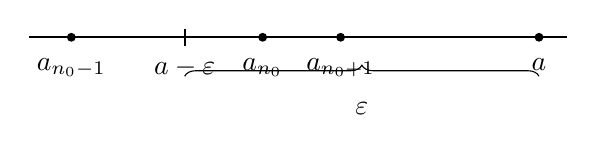
\begin{tikzpicture}[x=0.9cm,y=0.9cm,>=stealth]
  % --- choose positions (kept compact for letter paper) ---
  \def\xLeft{0}
  \def\xAe{2.2}
  \def\xAnz{3.3}
  \def\xAnzp{4.4}
  \def\xA{7.2}

  % number line
  \draw[thick] (\xLeft,0) -- (\xA+0.4,0);

  % tick at a-ε
  \draw[thick] (\xAe,0.12) -- (\xAe,-0.12);

  % points
  \fill (\xLeft+0.6,0) circle (1.6pt) node[below=4pt] {$a_{n_0-1}$};
  \fill (\xAnz,0)      circle (1.6pt) node[below=4pt] {$a_{n_0}$};
  \fill (\xAnzp,0)     circle (1.6pt) node[below=4pt] {$a_{n_0+1}$};
  \fill (\xA,0)        circle (1.6pt) node[below=4pt] {$a$};

  % label a-ε under tick
  \node[below=4pt] at (\xAe,0) {$a-\varepsilon$};

  % epsilon brace from a-ε to a
  \draw[decorate,decoration={brace,amplitude=4pt}]
    (\xAe,-0.55) -- (\xA,-0.55)
    node[midway,below=6pt] {$\varepsilon$};

  % optional: subtle note above (kept short)
  % \node[above=6pt] at ({(\xAe+\xA)/2},0) {$a-\varepsilon < a_n \le a$ for $n\ge n_0$};
\end{tikzpicture}
\end{center}

Thus,
\[
a_n \in N_\varepsilon(a)
\quad \text{for all } n \ge n_0.
\]
This is precisely the definition of convergence. Therefore,
\[
\lim_{n \to \infty} a_n = a.
\]
\end{proof}

% =========================================================
% Real Analysis — Sequences Completion Checklist
% =========================================================


\newpage


\begin{center}
    {\LARGE \textbf{Real Analysis — Sequences Completion Checklist}}\\[1em]
\end{center}

% =========================================================
\section*{I. Real Number Foundations}

\subsection*{Field \& Order Structure}

% ---------------------------------------------------------
% Toolkit
% ---------------------------------------------------------
\begin{tcolorbox}[title=Toolkit: Path]
\begin{tabular}{@{}p{0.28\textwidth}p{0.68\textwidth}@{}}
\textbf{Core items} & Key definitions/results introduced in this file.\\
\textbf{How to use} & Read the boxed items first; proofs and consequences follow.\\
\textbf{Dependencies} & Refer back to earlier sections as needed.\\
\end{tabular}
\end{tcolorbox}


\begin{itemize}
\item \checkbox Field axioms of $\mathbb{R}$
\item \checkbox Order axioms of $\mathbb{R}$
\item \checkbox Trichotomy Law
\item \checkbox Compatibility of order with addition
\item \checkbox Compatibility of order with multiplication
\end{itemize}

\subsection*{Absolute Value}

\begin{itemize}
\item \checkbox Definition of absolute value
\item \checkbox $|x| \ge 0$ and $|x| = 0 \iff x = 0$
\item \checkbox $|xy| = |x||y|$
\item \checkbox Triangle inequality
\item \checkbox Reverse triangle inequality
\end{itemize}

\subsection*{Suprema \& Infima}

\begin{itemize}
\item \checkbox Definition of upper bound
\item \checkbox Definition of lower bound
\item \checkbox Definition of supremum
\item \checkbox Definition of infimum
\item \checkbox Supremum is unique
\item \checkbox Completeness (Least Upper Bound Property)
\end{itemize}

\subsection*{Archimedean Property}

\begin{itemize}
\item \checkbox Archimedean property statement
\item \checkbox Equivalent forms
\item \checkbox Proof that $\frac{1}{n} \to 0$
\end{itemize}

% =========================================================
\section*{II. Basic Sequence Theory}

\subsection*{Definitions}

\begin{itemize}
\item \checkbox Definition of sequence ($\mathbb{N} \to \mathbb{R}$)
\item \checkbox Definition of convergence ($\varepsilon$–$N$ form)
\item \checkbox Negation of convergence
\end{itemize}

\subsection*{Fundamental Theorems}

\begin{itemize}
\item \checkbox Uniqueness of limits
\item \checkbox Convergent $\Rightarrow$ bounded
\end{itemize}

\subsection*{Algebra of Limits}

\begin{itemize}
\item \checkbox Sum rule
\item \checkbox Scalar multiple rule
\item \checkbox Product rule
\item \checkbox Quotient rule (nonzero limit)
\end{itemize}

\subsection*{Order Limit Theorems}

\begin{itemize}
\item \checkbox Limit preserves inequalities
\item \checkbox Squeeze theorem
\end{itemize}

% =========================================================
\section*{III. Structural Sequence Theory}

\subsection*{Monotone Sequences}

\begin{itemize}
\item \checkbox Definition of monotone increasing
\item \checkbox Definition of monotone decreasing
\item \checkbox Monotone Convergence Theorem
\end{itemize}

\subsection*{Subsequences}

\begin{itemize}
\item \checkbox Definition of subsequence
\item \checkbox $n_k$ strictly increasing
\item \checkbox Subsequence of convergent sequence converges to same limit
\item \checkbox Subsequence of subsequence lemma
\item \checkbox Index growth fact: $n_k \ge k$
\end{itemize}

\subsection*{Bolzano--Weierstrass}

\begin{itemize}
\item \checkbox Every bounded sequence has a convergent subsequence
\end{itemize}

% =========================================================
\section*{IV. Cauchy Theory \& Completeness}

\subsection*{Cauchy Sequences}

\begin{itemize}
\item \checkbox Definition of Cauchy sequence
\item \checkbox Convergent $\Rightarrow$ Cauchy
\item \checkbox Cauchy $\Rightarrow$ bounded
\item \checkbox Cauchy $\Rightarrow$ convergent (Completeness of $\mathbb{R}$)
\end{itemize}

% =========================================================
\section*{V. Limit Superior / Limit Inferior}

\begin{itemize}
\item \checkbox Definition of tail set
\item \checkbox Definition of $s_n = \sup_{k \ge n} a_k$
\item \checkbox Definition of $\limsup a_n$
\item \checkbox Definition of $\liminf a_n$
\item \checkbox $\limsup$ always exists (possibly $\pm\infty$)
\item \checkbox $\liminf$ always exists
\item \checkbox $\liminf \le \limsup$
\item \checkbox Convergence $\iff \limsup = \liminf$
\item \checkbox $\limsup$ equals largest subsequential limit
\item \checkbox $\liminf$ equals smallest subsequential limit
\end{itemize}

% =========================================================
\section*{VI. Subsequence Toolkit (Advanced)}

\begin{itemize}
\item \checkbox Finite Partition Convergence Principle
\item \checkbox Residue class convergence
\item \checkbox Even/odd convergence principle
\item \checkbox Dense subsequence criterion
\item \checkbox Diagonal subsequence lemma
\item \checkbox Inherited vs.\ reflected properties
\item \checkbox Tail properties
\item \checkbox Universal subsequence properties
\end{itemize}

% =========================================================
\section*{Final Mastery Check}

\begin{itemize}
\item \checkbox Prove Monotone Convergence from completeness
\item \checkbox Prove Bolzano--Weierstrass
\item \checkbox Prove Cauchy $\iff$ Convergent in $\mathbb{R}$
\item \checkbox Extract convergent subsequences intentionally
\item \checkbox Compute $\limsup$ and $\liminf$ in nontrivial examples
\item \checkbox Characterize convergence via $\limsup/\liminf$
\end{itemize}


\newpage


